\documentclass[acmsmall]{acmart}

\usepackage{mathtools,siunitx,booktabs,tikz,multirow,soul,comment,hyperref,amsbsy,amssymb,amsthm,amsfonts,bbm,textcomp,graphicx,wrapfig,float,subcaption,algorithm,algpseudocode}
\usepackage[table]{xcolor}
\usepackage[american]{babel}
\usepackage{natbib} 

\newtheorem{example}{Example}
\newtheorem{definition}{Definition}
\newtheorem{theorem}{Theorem}
\newtheorem{lemma}{Lemma}

\AtBeginDocument{%
  \providecommand\BibTeX{{%
    Bib\TeX}}}

\setcopyright{acmlicensed}
\copyrightyear{2026}
\acmYear{2026}
\acmDOI{XXXXXXX.XXXXXXX}

\acmJournal{TIST}
\acmVolume{0}
\acmNumber{0}
\acmArticle{0}
\acmMonth{0}

\begin{document}

\title{Good $\not=$ Trustworthy: Beyond performance-wise Client Contribution Evaluation in Federated Learning}

\author{Bal{\'a}zs Pej{\'o}}
\affiliation{%
  \institution{Laboratory of Cryptography and Systems Security (CrySyS), Department of Networked Systems and Services (HIT), Faculty of Electrical Engineering and Informatics (VIK), Budapest University of Technology and Economics (BME) \& HUN-REN-BME Information Systems Research Group, HUN-REN Hungarian Research Network}
  \city{Budapest}
  \country{Hungary}}
\email{pejo@crysys.hu}

\author{Zsuzsanna Fl{\'o}ra Ulrich}
\affiliation{%
  \institution{Department of Networked Systems and Services, Budapest University of Technology and Economics}
  \city{Budapest}
  \country{Hungary}
}

%\renewcommand{\shortauthors}{Pejo \& Ulrich}
%\renewcommand{\shorttitle}{Good $\not=$ Trustworthy}

\begin{abstract}
    Federated learning offers a privacy-friendly collaborative learning framework, yet its success, like any joint venture, hinges on the contributions of its participants. Existing client evaluation methods predominantly focus on standard performance metrics, such as accuracy or loss, which represent only one dimension of a machine learning model's overall utility. In contrast, this work investigates the critical, yet overlooked, issue of evaluating client contributions towards a model's trustworthiness. Specifically, we consider two robustness (reliability and resilience capture the tolerance to noisy data and adversarial examples, respectively) and fairness (measured via demographic parity and equalized odds) metrics. Moreover, we consider privacy (via membership inference attack). \\    
    To quantify these multifaceted contributions, we employ the lightweight Leave-One-Out and the state-of-the-art GTG Shapley value approximation. Through extensive empirical evaluation across three domains (tabular, computer vision, and natural language processing), we reveal that these trustworthiness dimensions are not captured by standard performance. In fact, they are frequently anti-correlated with it. No single client excels universally, highlighting a critical flaw in current evaluation schemes. Furthermore, beyond passive scoring we utilize these values by reweighting the clients to steer the global model toward a chosen trustworthiness dimension. This server-side intervention matches or exceeds standard local paradigms such as adversarial training or fair regularization on the targeted dimension, albeit at a quantifiable cost to predictive accuracy. 
\end{abstract}

\begin{CCSXML}
<ccs2012>
   <concept>
       <concept_id>10002978.10002991.10002995</concept_id>
       <concept_desc>Security and privacy~Privacy-preserving protocols</concept_desc>
       <concept_significance>500</concept_significance>
       </concept>
   <concept>
       <concept_id>10010147.10010257.10010341</concept_id>
       <concept_desc>Computing methodologies~Model verification and validation</concept_desc>
       <concept_significance>500</concept_significance>
       </concept>
   <concept>
       <concept_id>10010147.10010257</concept_id>
       <concept_desc>Computing methodologies~Machine learning</concept_desc>
       <concept_significance>300</concept_significance>
       </concept>
   <concept>
       <concept_id>10010405.10010481.10010482</concept_id>
       <concept_desc>Applied computing~Multi-criterion optimization and decision-making</concept_desc>
       <concept_significance>300</concept_significance>
       </concept>
 </ccs2012>
\end{CCSXML}

\ccsdesc[500]{Security and privacy~Privacy-preserving protocols}
\ccsdesc[500]{Computing methodologies~Model verification and validation}
\ccsdesc[300]{Computing methodologies~Machine learning}
\ccsdesc[300]{Applied computing~Multi-criterion optimization and decision-making}

\keywords{Federated Learning, Contribution Evaluation, Trustworthiness, Fairness, Robustness, Privacy}

\received{2026}
\received[revised]{2026}
\received[accepted]{2026}

\maketitle

\section{Introduction}

The proliferation of digital technology has enabled the collection of vast amounts of user data, fueling the rapid advancement of Machine Learning (ML). However, this data is often fragmented into isolated silos, limiting the full potential of ML to entities with access to large, centralized datasets and potentially leading to suboptimal models. Naive data pooling to overcome this fragmentation is often infeasible, as it can lead to severe privacy violations (i.e., GDPR) and erode competitive advantages for businesses where data is a key asset. To address these challenges and democratize AI, Federated Learning (FL)~\cite{mcmahan2017communication} has emerged as a powerful paradigm. It enables multiple parties to collaboratively train a shared model without exposing their raw data, thus preserving privacy while improving model generalization. 

However, managing this collaborative process is notoriously difficult due to extreme statistical heterogeneity (non-IID data distributions) among clients, which inherently skews local model updates~\cite{kairouz2021advances}. An appropriate mechanism to manage this heterogeneity is data and client evaluation, which intersects with several dimensions of trustworthiness. For instance, quantifying clients is essential for ensuring accountability and transparency in the federation~\cite{siomos2023contribution}, while related valuation techniques that assess feature importance are a cornerstone of model explainability and interpretability~\cite{gunning2019xai}. Furthermore, client data directly impacts model privacy~\cite{liu2021machine}, fairness~\cite{mehrabi2021survey}, reliability~\cite{goldblum2022dataset}, and resilience~\cite{ibitoye2019threat}. These dimensions are often intertwined, creating a complex web of trade-offs~\cite{liu2020privacy, shaham2023holistic, li2024triangular}. In this paper, we focus on these four critical objectives:

\begin{itemize}
    \item \textbf{Fairness}: The model avoids discrimination against groups based on sensitive attributes.
    \item \textbf{Reliability}: The model performs consistently, across noisy or corrupted data.
    \item \textbf{Resilience}: The model maintains its performance regarding adversarial attacks.
    \item \textbf{Privacy:} The model is less prone to leak information about its training data.
\end{itemize}

From a regulatory and governance perspective, our focus directly tackles the core mandates of the European Trustworthy AI framework~\cite{kaur2022trustworthy} and the European Union's Artificial Intelligence Act (AI Act). Under these regulations, particularly for high-risk applications, demonstrating technical robustness, cybersecurity (resilience), strict data governance (privacy), and non-discrimination (fairness) is no longer merely an ethical guideline but a strict legal compliance requirement. By explicitly quantifying these exact dimensions, our evaluation framework provides a verifiable mechanism to ensure that collaborative AI systems are built to meet these stringent regulatory standards from the ground up.

Despite the importance of these multifaceted goals, the critical flaw of all existing evaluation methods is that they almost exclusively rely on a single performance metric, typically accuracy or model loss~\cite{naidu2023review}. This creates a narrow, and potentially misleading, view of a client's true value. For instance, most works apply data valuation with the singular goal of improving training efficiency (e.g., faster convergence or a more accurate model) by assigning higher/lower weights or selecting clients more/less frequently based on performance quality~\cite{gao2025fedcon, sani2026fedssv}. This paper challenges this performance-centric paradigm, arguing that a client's contribution to model trustworthiness is an equally, if not more, important consideration.

\subsubsection*{Contributions}

We conduct a multifaceted analysis of client contributions in FL, extending the evaluation to key trustworthiness metrics. Our primary contributions are as follows:

\begin{itemize}
    \item We evaluate the contribution of FL clients based on seven distinct metrics corresponding to four trustworthy dimensions: performance (measured by accuracy and loss), fairness (measured by demographic parity and equalized odds), robustness (measured by reliability (tolerance to noise) and resilience (resistance against adversarial examples)), and privacy (via membership inference attack).
    \item We show that these trustworthy AI pillars are not reducible to performance: the scores allocated to the same clients are frequently uncorrelated or even anti-correlated with the performance scores, while metrics within a conceptual family (e.g., the two fairness or the two robustness scores) form tightly correlated clusters.
    \item We apply two distinct and well-established contribution evaluation schemes, the lightweight Leave-One-Out and the state-of-the-art Guided-Truncated-Gradient Shapley approximation, to demonstrate that our findings are present across different valuation methodologies.
    \item We conduct a systematic empirical study across three different ML domains (tabular data, computer vision, and natural language processing) to validate our conclusions.
    \item We demonstrate the practical utility of our framework by implementing an actionable client-weighting mechanism, illustrating how trustworthiness scores can be utilized to actively steer the global model toward improving these trustworthiness pillars. 
\end{itemize}

Our core finding is that client rankings differ dramatically across evaluation metrics. We provide compelling evidence that clients who are highly valuable for model performance can be neutral or even detrimental to its fairness, reliability, resilience, or privacy, and vice versa. 

\subsubsection*{Organization}

The remainder of this paper is organized as follows. Section~\ref{sec:RW} reviews related work, while in Section~\ref{sec:mod}, we detail our multifaceted evaluation metrics. In Section~\ref{sec:exp}, we describe our experimental setup and present our empirical results, findings, and the client weighting application. Finally, we discuss the broader implications of our work and conclude the paper in Section~\ref{sec:con}.

\section{Related Works}
\label{sec:RW}

\subsection{Trustworthy AI}

As machine learning systems transition from research to integral components of high-stakes societal functions, the development paradigm has evolved to demand a holistic view of model validity. While optimizing for predictive performance remains foundational, it must now be tightly coupled with ensuring overall trustworthiness~\cite{huang2024flsurvey}. This is particularly critical in domains where model failures can have severe economic and social consequences. Within this work, we evaluate overall model validity across four core pillars: 1) Performance, which ensures the fundamental predictive utility and accuracy of the system; 2) Fairness, which seeks to prevent unjust or prejudicial treatment; 3) Robustness, which guarantees both reliable operation under uncertain conditions and resilience against adverse manipulations; and 4) Privacy, which protects against the extraction of sensitive training data.

\subsubsection*{Fairness}

Machine learning models, despite their mathematical objectivity, are trained on data generated by a society with historical and systemic biases~\cite{mehrabi2021survey}. Consequently, these models can inadvertently learn, reproduce, and even amplify these biases, leading to discriminatory outcomes in high-stakes applications~\cite{hall2022systematic}. It is not only an ethical imperative but also an emerging legal requirement, making it a critical component of trustworthy AI~\cite{wachter2020bias}. The concept of fairness is realized through various quantitative metrics, each capturing a different notion of equity. In this work, we focus on two well-established group fairness criteria. First, we consider Demographic Parity (DP)~\cite{calders2009building}, which requires that the model’s predictions be statistically independent of the sensitive attribute. Second, we incorporate Equalized Odds (EO)~\cite{hardt2016equality}, which requires that the prediction be conditionally independent of the sensitive attribute given the true label, thereby enforcing comparable true positive and false positive rates across sensitive groups. 

\subsubsection*{Robustness}

While often discussed together, reliability and resilience are distinct parts of robustness within Trustworthy AI that address different types of data perturbations~\cite{fawzi2016robustness}. Reliability concerns a model's ability to perform consistently when faced with naturally occurring, random noise or data corruption~\cite{shannon1948}. This simulates real-world challenges like blurry images from camera shake, background noise in audio recordings, or simple data entry errors and the occurring white noise during communication. Resilience, in contrast, measures a model's tolerance against deliberately crafted, worst-case perturbations, commonly known as adversarial examples~\cite{goodfellow2014explaining}. These attacks introduce small, often imperceptible changes to an input with the specific goal of deceiving the model and causing a misclassification. In this work, we use the well-known method called Projected Gradient Descent (PGD)~\cite{madry2017towards} to generate such samples.

Despite this clear conceptual difference, the two terms are frequently conflated in the literature, often grouped under the umbrella term robustness. This confusion is reflected in the metrics used for their evaluation. For instance, Mean Corruption Error~\cite{mCE} and Effective Robustness~\cite{effectiverelative} focus on reliability, while Adversarial Accuracy~\cite{23metric} is tailored to measure resilience. Besides this confusion, a more significant limitation is that most of these metrics are heavily confounded by the model's accuracy. A model with higher general performance will almost always score better on corrupted or adversarial data, making it difficult to discern whether the model is truly more reliable or simply more accurate to begin with. This effect makes it challenging to evaluate a client's specific contribution to the model's reliability or resilience, separate from their contribution to its overall performance. To address this gap, our work explicitly treats reliability and resilience as separate objectives. We seek to evaluate them using methods that isolate these properties from the model's general predictive accuracy. This approach allows for a more direct and nuanced assessment of a client's contribution to protecting the model against either naturally occurring random noise or specific adversarial threats.

\subsubsection*{Privacy}

While FL inherently provides a baseline level of confidentiality by keeping raw data localized, this architectural separation is fundamentally insufficient to guarantee true privacy~\cite{liu2021machine}. To mitigate the potential vulnerabilities, the ML community has turned to rigorous statistical guarantees, most notably Differential Privacy~\cite{pejo2022guide}. However, privacy does not exist in a vacuum; it introduces complex, well-documented trade-offs with the other pillars of Trustworthy AI~\cite{zhang2023survey}. For instance, defenses are known to degrade not only overall predictive performance but also fairness~\cite{rafi2024fairness} or robustness~\cite{zhang2023survey}. While this tension is widely studied at the global model level, there remains a significant gap in understanding how individual participants shape this dynamic. The authors in~\cite{duddu2024shapr} used a Shapley/LOO value as a per-sample membership-privacy metric; we instead quantify each client's contribution to the global model's privacy preservation.

\subsection{Contribution Evaluation}

Evaluating the contribution of individual clients to a collaborative model is a critical task. While a handful of strategies exist to tackle this~\cite{huang2020exploratory,jiang2023opendataval}, the cornerstone technique for most quality assessment problems within FL~\cite{jain2020overview} is the Shapley Value (SV)~\cite{winter2002shapley,rozemberczki2022shapley}. Originating from cooperative game theory, the Shapley Value of a client is defined as their average marginal contribution to the model's utility across all possible subsets (coalitions) of clients. While it possesses desirable axiomatic properties that guarantee a fair and unique distribution, its primary drawback is its computational complexity, which makes exact computation infeasible for typical FL scenarios. Consequently, a variety of approximation methods have been developed, such as Monte-Carlo based approaches and gradient-based techniques~\cite{ghorbani2019data,liu2022gtg}, which aim to estimate the value in a computationally tractable manner.

\subsubsection*{Fairness}

The term "fairness" carries a dual meaning in this context, referring to both the properties of the reward allocation scheme (game-theoretic fairness~\cite{rabin1993incorporating}) and the statistical properties of the machine learning model (algorithmic fairness~\cite{kleinberg2018algorithmic}). This creates a twofold intersection with contribution evaluation. First, one can assess the fairness of the allocation scheme itself. The Shapley Value is axiomatically the only "fair" reward allocation method; thus, any other scheme, including its approximations, inevitably compromises on some aspect of this game-theoretic fairness. Furthermore, evaluating clients across multiple trustworthy dimensions simultaneously raises the question of how to handle multi-objective attributions. Recent theoretical work~\cite{biccari2026fair} has demonstrated that for multi-output or multi-objective scenarios, calculating Shapley values component-wise (i.e., evaluating each objective independently) is the mathematically rigorous approach to satisfy fairness axioms. This provides strong theoretical backing for our methodology, as we independently compute contribution scores for performance, fairness, robustness, and privacy, ensuring that the attribution for each dimension remains distinct and valid.

Second, one can evaluate the algorithmic fairness of the trained model and allocate value to clients based on their contribution to that specific objective. Since the quality of data and clients has long been understood to extend beyond simple accuracy~\cite{wang1996beyond}, this second interpretation is our focus. Our work is inspired by recent efforts to view algorithmic fairness through a data-quality lens. The authors in~\cite{arnaiztowards} assign importance scores for individual training samples based on their contribution to a model's fairness, rather than its performance. We bridge this concept with FL, extending the unit of analysis from a single data point to an entire client. 

\subsubsection*{Robustness}

The relationship between contribution evaluation and model robustness is also multifaceted and heavily researched. On one hand, studies have explored how the evaluation process itself can be vulnerable; for example, contribution scores can be manipulated through data poisoning attacks, highlighting a lack of resilience in the evaluation schemes themselves~\cite{xu2024ace,pejo2025fragility}. Beyond deliberate adversarial manipulations, the inherent reliability of the contribution scores remains a significant concern. Because SV estimates rely on stochastic approximation algorithms and randomized model training processes, they often suffer from instability. Recent literature has explored this uncertainty by examining the impact of FL aggregation techniques~\cite{pejo2025fragility}, the variance within the training mechanisms~\cite{goldwasser2024stabilizing}, and the consistency of different value functions against natural noise~\cite{wang2023data}. Furthermore, these evaluation frameworks can be game-theoretically fragile; Shapley-based allocations might incentivize participants to strategically split their data to maximize individual payouts, degrading the global model in a classic "tragedy of the commons" scenario~\cite{qi2024mechanism}. 

Crucially, the prevailing literature overwhelmingly focuses on ensuring the reliability and resilience of the evaluation schemes themselves. Our work addresses the inverse problem. First, we shift the focus to utilizing these schemes to measure the reliability and resilience of the global model, quantifying a client's specific contribution to these defensive objectives alongside their impact on performance, fairness, and privacy. Second, while contribution-weighted aggregation is well studied for performance and robustness~\cite{sun2023shapleyfl,tastan2024redefining,guan2022few,otmani2024fedsv}, we extend this dynamic client-weighting intervention across all trustworthy dimensions to actively steer model convergence.

\begin{wraptable}{r}{0.5\textwidth}
    \vspace{-1cm}
    \centering
    \small
    \begin{tabular}{c|l}
        Symbol & Description \\
        \hline
        $k\in[K]$ & FL clients \\
        $M_k^t$ \& $M^t$ & Local \& global models in round $t$ \\
        $D_k$ \& $D^\prime$ & Training \& Testing datasets \\
        $x$ \& $y$ & Data sample \& label \\
        $n$ \& $a$ & Gaussian \& malicious noise \\
        & Evaluation function for scoring \\
        $v(\cdot)$ & $v \in \{\mathtt{acc}, \mathtt{loss}, \mathtt{priv},$ \\
        & $\mathtt{fairDP}, \mathtt{fairEO}, \mathtt{rel}, \mathtt{res}\}$ \\
        \multirow{2}{*}{$\mathtt{CS}^t_v$} & Contribution score in round $t$ \\
        & $\mathtt{CS}^t_v\in\{\mathtt{GTG}^t_v, \mathtt{LOO}^t_v\}$ \\
    \end{tabular}
    \caption{Notations used in the paper.}
    \label{tab:notations}
    \vspace{-1cm}
\end{wraptable}

\section{Trustworthiness Scores}
\label{sec:mod}

\subsubsection*{Notation}

The objective of ML is to iteratively (i.e., $1\leq t \leq T$) train a model $M(\theta)^t$ with parameters $\theta=\{\theta_1,\dots,\theta_m\}$ and with empirical loss function $\mathcal{L}(x,\theta)$ (where $x$ is a sample) such that the prediction is enhanced with respect to a specific task. During training the empirical loss is minimized: $\min_\theta \sum_{x\in D}\mathcal{L}(x,\theta)$. A summary of the utilized symbols are presented in Table~\ref{tab:notations}, which also contains the variables specific to the proposed evaluation schemes.

\subsubsection*{Contribution Evaluation}

Before defining our trustworthiness scores, we first outline the classical approach to client evaluation, which is based on model performance. The gold standard for this task is the Shapley Value: for a set of $K$ clients, the $\mathtt{SV}$ for client $k$ is defined in the left side of Eq.~\eqref{eq:GTG-LOO}, where $\Pi(K)$ is the set of all permutations of the $K$ clients, and $\pi_{<k}$ denotes the set of clients preceding $k$ in a given permutation $\pi$. Note, we present the formula to be suitable with evaluation functions $v(\cdot)$ where higher values mean better model. As calculating the exact value requires exponentially many model trainings (one for each possible client combination), we utilize Data Shapley~\cite{ghorbani2019data} instead, which only requires a single model to be trained: in each round all possible combination of gradients are used to update the model and the marginal differences are computed by comparing these intermediate submodels. The final score is the accumulated score from all rounds. Guided-Truncated-Gradient Shapley ($\mathtt{GTG}$)~\cite{liu2022gtg}, the SotA approximation technique enhances this by 1) skipping entire rounds of FL if the global model's improvement is negligible ($<\epsilon_1$), 2) it samples a portion ($\epsilon_2$) of all subset from all possible client permutations (such that each client is equal times in the early places), and 3) for each sampled permutation, it only evaluates the marginal contributions of a client if they exceed a minimum threshold ($>\epsilon_3$). 

\begin{equation}
    \label{eq:GTG-LOO}
    \mathtt{SV}_v(k) = \frac{1}{|K|!} \sum_{\pi \in \Pi(K)} \left( v(\pi_{<k} \cup \{k\}) - v(\pi_{<k}) \right)
    \hspace{1cm}
    \mathtt{LOO}_v(k) = v([K]) - v([K]\setminus\{k\})
\end{equation}

Another, even more lightweight and widely used alternative approach that we also utilize in this paper is the Leave-One-Out ($\mathtt{LOO}$) heuristic~\cite{evgeniou2004leave}. While less principled than GTG, it is computationally much cheaper. A client's contribution is simply the change in utility observed when they are removed from the grand coalition, as shown in the right side of Eq.~\eqref{eq:GTG-LOO}. 

\subsubsection*{Performance Scoring}

As far as we know, almost without exception, the utility function $v(\cdot)$ in the FL literature is defined by a standard predictive performance metric, namely accuracy or loss. Within our study, we evaluate both. However, because contribution scoring frameworks necessitate a utility function where higher values indicate better outcomes, raw loss cannot be used directly. Therefore, we apply an exponential decay transformation to the empirical loss, monotonically mapping it into a $[0, 1]$ utility range comparable to accuracy. This performance evaluation is formalized in Eq.~\eqref{eq:perf}. Crucially, we subsequently adapt these evaluation schemes to capture the model's fairness, robustness, and privacy, independently of its underlying predictive performance. A visual illustration of what some scores capture is presented in Fig.~\ref{fig:illustrate}, while the high-level pseudo-code encapsulating our scoring methodology is presented in Alg.~\ref{alg:alg}. 

\begin{equation}
    \label{eq:perf}
    \mathtt{acc}(M) = \Pr_{x\in D^\prime}[M(x) = y]
    \hspace{2cm}
    \mathtt{loss}(M) = e^{-\frac{1}{|D^\prime|}\sum_{x\in D^\prime}\mathcal{L}(x,\theta)}
\end{equation}

\begin{figure}[t]
    \begin{minipage}[b]{0.55\textwidth}
        \centering
        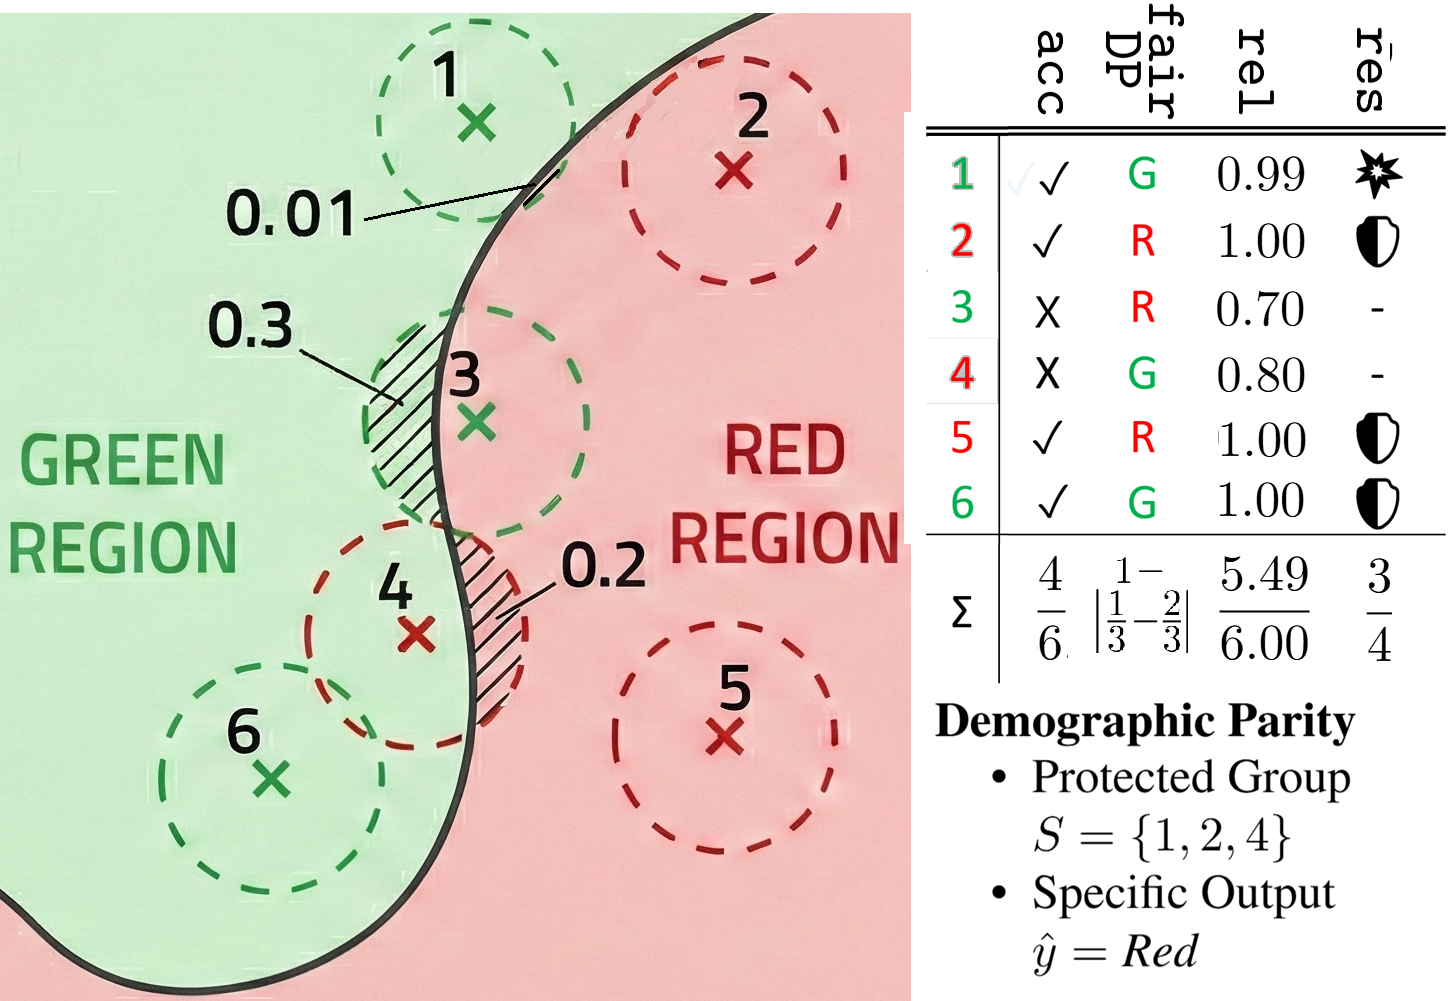
\includegraphics[width=\linewidth]{figs/GeminiExcel.png}
    \end{minipage}
    \hfill
    \begin{minipage}[b]{0.4\textwidth}
        \begin{algorithm}[H]
            \caption{Assigning scores to clients in round $t$.}
            \label{alg:alg}
            \flushleft
            \textbf{Input}: $M^{t-1}$, $D_k$, $D^\prime$ \\
            \textbf{Output}: $\mathtt{CS}^t_{v}(D_k)$
            \begin{algorithmic}[1]
            \For{each client $k \in [K]$}
                \State $M^t_k$ $\leftarrow$ $Train(M^{t-1})$
                \State Share $M_k^t$ with the server
            \EndFor
            \For{$\mathtt{CS}\in$ $\{\mathtt{GTG}$, $\mathtt{LOO}\}$}
                \For{$v\in\{$ $\mathtt{acc}$, $\mathtt{loss}$, $\mathtt{fairDP}$, $\mathtt{fairEO}$, $\mathtt{rel}$, $\mathtt{res}$, $\mathtt{priv}\}$}
                \State $[\mathtt{CS}^t_v(D_k)]_1^K$ $\leftarrow$ $[M_k^t]_1^K$
                \EndFor
            \EndFor
            \end{algorithmic}
        \end{algorithm}
    \end{minipage}
    \caption{Example to illustrate what the different trustworthiness scores capture based on $D^\prime=\{(1,G),(2,R),(3,G),(4,R),(5,R),(6,G)\}$. While the model is $0.67$ accurate, its trustworthiness scores are widely different, e.g., $\mathtt{fairDP}(M)=0.67$ (a demographic-parity gap of $0.33$) where the protected group is the powers of two ($S=\{1,2,4\}$) and 'Red' is the target class. Regarding reliability, the model might flip the prediction of three $(1,3,4)$ samples with various probabilities, an average change chance of $0.09$, i.e., $\mathtt{rel}(M)=5.49/6\approx0.92$. Regarding resilience, the attacker is successful once $(1)$ out of the four $(1,2,5,6)$ correctly classified samples, an attack success rate of $0.25$, i.e., $\mathtt{res}(M)=0.75$.}
    \label{fig:illustrate}
\end{figure}

\subsubsection*{Fairness Scoring}

Our fairness-related evaluation is based on two group fairness criteria, both relying on the test dataset. First, we consider Demographic Parity (Def.~\ref{def:DP}), which requires the model to predict the target outcome at equal rates across all demographic groups, regardless of sensitive attributes. Second, we consider Equalized Odds (Def.~\ref{def:EO}), which ensures that the predictions are conditionally independent of the sensitive attribute given the true label. Note, EO requires both the True Positive Rate (TPR) and the False Positive Rate (FPR) to be identical across all sensitive groups.

We assign the Demographic Parity-based fairness score to model $M$ by taking the absolute difference between the conditional probabilities in Def.~\ref{def:DP}, as formalized in Eq.~\eqref{eq:fairDP}. Similarly, for Equalized Odds, the model must balance disparities across both TPR and FPR, depending on the true label $y$. To capture this in a single metric, we calculate the absolute disparity for both rates and average them across all possible labels $Y$, as formalized in Eq.~\eqref{eq:fairEO}. Crucially, by subtracting these absolute disparities from 1, we transform them into a continuous $[0,1]$ utility range where higher values indicate a fairer model. 


\begin{definition}[Demographic Parity~\cite{calders2009building}]
    \label{def:DP}
    For a sensitive group $S\subset D^\prime$ and for a specific output $\hat{y}$, DP requires the following:
    \begin{equation*}
         \Pr_{x_i\in D^\prime}[M(x_i)=\hat{y} \mid x_i\in S] = \Pr_{x_i\in D^\prime}[M(x_i)=\hat{y} \mid x_i\notin S]
    \end{equation*}
\end{definition}

\begin{definition}[Equalized Odds~\cite{hardt2016equality}]
    \label{def:EO}
    For a sensitive group $S\subset D^\prime$, a specific output $\hat{y}$, and any true label $y \in \{0, 1\}$, EO requires the following conditional independence:
    \begin{equation*}
        \Pr_{(x_i,y_i)\in D^\prime}[M(x_i) = \hat{y} \mid x_i\in S, y_i=y] = \Pr_{(x_i,y_i) \in D^\prime}[M(x_i) = \hat{y} \mid x_i\notin S, y_i=y]
    \end{equation*}
\end{definition}

\begin{equation}
    \label{eq:fairDP}
    \mathtt{fairDP}(M) = 1 - \left| \Pr_{x\in D^\prime}[M(x_i)=\hat{y} \mid x_i\in S] - \Pr_{x\in D^\prime}[M(x_i)=\hat{y} \mid x_i\notin S] \right|
\end{equation}

\begin{equation}
    \label{eq:fairEO}
    \begin{split}
    \mathtt{fairEO}(M) = \\
    1 - \frac{\sum\limits_{y\in Y} \left| \Pr\limits_{(x_i,y_i)\in D^\prime}[M(x)=\hat{y} \mid x_i\in S, y_i=y] - \Pr\limits_{(x_i,y_i)\in D^\prime}[M(x_i)=\hat{y} \mid x_i\notin S, y_i=y] \right|}{|Y|}
    \end{split}
\end{equation}

\subsubsection*{Reliability Scoring}

To measure reliability, we assess the stability of a model's predictions when subjected to naturally occurring, random noise. To simulate this, we perturb each test sample $x\in D^\prime$ with noise drawn from a Gaussian distribution, $n\sim \mathcal{N}(0,\sigma)$, and compare the prediction between the original and the perturbed input, as formalized in Eq.~\eqref{eq:rel}. A key feature of this reliability metric is its strict independence from the model's predictive accuracy; it purely evaluates the consistency of the output, regardless of its correctness. In practice, rather than computing an intractable analytical expectation, we estimate this probability empirically by applying a fixed number of independent random perturbations to each sample. In line with the other trustworthiness scores, it is bounded in the range $[0, 1]$, where $1$ indicates perfect reliability (meaning the model's predictions are completely unaffected by the Gaussian noise).

\begin{equation}
    \label{eq:rel}
    \mathtt{rel}(M) = \Pr_{x\in D^\prime, n\sim\mathcal{N}(0,\sigma)}[M(x) = M(x+n)]
\end{equation}

\subsubsection*{Resilience Scoring}

In contrast to reliability, which measures stability against random noise, our resilience metric quantifies a model's defense against a deliberate, worst-case adversarial attack. To evaluate this, we adopt a standard methodology from the adversarial machine learning literature by subjecting the trained model to Projected Gradient Descent (PGD)~\cite{madry2017towards}. PGD is designed to find a malicious perturbation, $a$, that induces a misclassification, strictly constrained within a fixed noise threshold (e.g., an $\ell_p$-norm bound $\|a\|_p \leq \epsilon$). To ensure this metric isolates resilience from general performance, the resilience score is calculated exclusively based on the attack's failure rate on \textit{already correctly classified} samples, as defined in Eq.~\eqref{eq:res}. Consequently, a score of $0$ implies a maximal attack success rate and minimal model resilience, while $1$ indicates a perfect defense within the allowed $\epsilon$-boundary within the $p$-norm.

\begin{equation}
    \label{eq:res}
    \mathtt{res}(M) = 1 - \Pr_{(x,y) \in D^\prime}\big[ M(x+a) \neq y \bigm| M(x)=y, \|a\|_p \leq \epsilon \big]
\end{equation}

\subsubsection*{Privacy Scoring}

We utilize Membership Inference Attacks (MIAs)~\cite{bai2024membership} to empirically quantify a model's privacy leakage. However, evaluating this within a federated contribution-scoring framework presents a unique methodological challenge. First, the server lacks access to the clients' raw training data, meaning genuine training members are unavailable for a standard attack evaluation. Second, privacy leakage is exclusively a property of training data; yet, to fairly evaluate and compare different client coalitions, we must use the exact same shared evaluation dataset ($D^\prime$) that we use for performance, fairness, and robustness. To reconcile this, we get inspiration from recent findings regarding LLM benchmarking~\cite{hardt2025emerging}: our protocol employs a uniform shadow fine-tuning approach to construct a controlled proxy. We deterministically partition the server's test set $D^\prime$ into a designated member set $D^\prime_\in$ and a complementary non-member set $D^\prime_{\not\in}$. Before evaluating an aggregated coalition model $M$, we briefly fine-tune it exclusively on $D^\prime_\in$. This intentionally induces measurable memorization (overfitting) on these specific samples, effectively converting them into "training" data for the purpose of the attack. Because this fine-tuning step is applied identically to every evaluated model subset, it guarantees a standardized agreement: all coalitions are evaluated for privacy leakage using the exact same underlying data baseline. We emphasize that this protocol does not measure leakage of the clients' actual training records, which remain the clients' own concern. From the standpoint of the central coordinator, the relevant quantity is the model's propensity to memorize newly seen data once fine-tuned; this is precisely what the uniform shadow protocol quantifies.

In this work we use the MIA proposed by Yeom et al.~\cite{yeom2018privacy}. Taking the maximum of the Area Under the Receiver Operating Characteristic Curve (AUC) achieved across the classifier, we define the privacy score in Eq.~\eqref{eq:priv}. By scaling, an $\text{AUC} = 0.5$ (indicating random guessing by the attacker) yields a perfect $\mathtt{priv}(M) = 1$ (no leakage). Conversely, a perfect attack ($\text{AUC} = 1.0$) yields $\mathtt{priv}(M) = 0$. Crucially, this privacy metric focuses on the delta of the attack success (scaled from the AUC), which is designed to minimize its confounding with the model's baseline predictive accuracy.

\begin{equation}
    \label{eq:priv}
    \mathtt{priv}(M) = 2 \cdot (1 - \max\{0.5,\text{AUC}\})
\end{equation}

\section{Experiments}
\label{sec:exp}

\subsubsection*{Setup}

To ensure our findings are generalizable, we conduct experiments across three settings: using CelebA~\cite{liu2015faceattributes} with a CNN~\cite{krizhevsky2012imagenet} for Computer Vision, using IMDB~\cite{maas-EtAl:2011:ACL-HLT2011} with a USE encoder~\cite{use} for Natural Language Processing, and using ADULT~\cite{becker1996adult} with an MLP~\cite{rumelhart1985learning} model for Tabular data. While we aim for performance-free metrics to measure the trustworthiness contributions, the underlying model should be accurate, as that is the point of the collaboration after all. Hence, we performed a hyperparameter optimization; the parameters are shown in Tab.~\ref{tab:hyper}. The training commences for ten rounds but in our score computation we disregard the first. Since it corresponds to training an untrained model, the corresponding change would dominate the rest and would skew the scoring results. We simulate a cross-silo setting with $K=4$ and $K=20$ clients. These small numbers are chosen so the individual client contributions remain meaningful, as scores tend to diminish with a large number of participants. 

To model realistic data heterogeneity, we evaluate clients under both IID and non-IID data distributions (using a Dirichlet distribution with $\alpha=0.5$). For aggregation we applied FedAVG and all experiments are repeated 5 fold. We deliberately fix the aggregator: prior work has shown that contribution scores themselves shift under different aggregation rules~\cite{pejo2025fragility}, so holding FedAVG constant isolates the trustworthiness effects that are the subject of this study. The implementation is based in Python using the Flower framework and TensorFlow, our code is available as open-source under the MIT License: \url{https://anonymous.4open.science/r/FL_trust-45DF/}.

\begin{table}[!t]
    \footnotesize
    \centering
    \begin{tabular}{|l||c|c|c|}
        \hline
        \textbf{Property} & \textbf{ADULT} & \textbf{CelebA} & \textbf{IMDB} \\
        \hline\hline
        Train / Test & 40K / 10K & 30K / 5K & 20K / 5K \\
        \hline
        Input & 108 & (64, 64, 3) & 512 (USE) \\
        Model & MLP (256, 128, 64) & CNN (32, 64, 128) + FC (128) & MLP (128, 64) \\
        Act. func. & ReLU + sigmoid & MaxPool + ReLU + softmax & ReLU + softmax \\
        Optimizer & Adam & Adam & Adam \\
        LR / DO & $1\times10^{-3}$/0.1/0.05 & $1\times10^{-3}$/0.2/0.3/0.3 & $1\times10^{-3}$/-- \\
        $L_2$ Reg & $1\times10^{-4}$ & $5\times10^{-4}$ & -- \\
        Norm & Layer & Batch & -- \\
        Loss & Binary CCE & Sparse CCE & Sparse CCE \\
        \hline
    \end{tabular}
    \caption{Datasets and model configurations used in the experiments. }
    \label{tab:hyper}
\end{table}

The parameters for the GTG approximations are $\epsilon_1=0.001$, $\epsilon_2=0.05$, and $\epsilon_3=0.002$. For reliability, we inject Gaussian noise with a standard deviation of $\sigma=0.1$ and simulate it 100 times. For robustness, $\ell_\infty$-PGD was used with step size $\alpha=0.007$, $\varepsilon=0.3$ with 40 rounds for ADULT, step size $\alpha=0.0025$, $\varepsilon=0.01$ with 40 rounds for CelebA (the standard $\varepsilon=0.03$ saturates resilience to $0$, so we evaluate CelebA at the smaller, scale-matched $\varepsilon=0.01$), and step size $\alpha=0.00125$, $\varepsilon=0.005$ with 10 rounds for IMDB (attacked in the USE-embedding space; $\varepsilon$ is calibrated on the converged baseline to a mid-range resilience, as the legacy $\varepsilon=0.0015$ left the model essentially unperturbed while $\varepsilon\geq0.01$ saturates resilience to $0$). Regarding fairness, we utilize the \texttt{sex} attribute as the sensitive feature for the ADULT and CelebA datasets; since IMDB lacks such sensitivity annotation, we disregarded it for this purpose. For the privacy evaluation, the target member set $D^\prime_\in$ comprises $50\%$ of the test samples, drawn via a stratified, round-specific deterministic split, while the remaining half forms the non-member set $D^\prime_{\not\in}$. To induce the necessary memorization baseline, the tested models are first fine-tuned on $D^\prime_\in$ for two epochs using the Adam optimizer (learning rate $10^{-3}$, batch size $16$). This small batch size is chosen deliberately to maximize the number of gradient steps per epoch, thereby sharpening the fine-tuning signal. Next, inspired by~\cite{yeom2018privacy}, a five-dimensional feature vector is extracted from the model's behavior on the samples: $[\mathcal{L}(\theta), \mathcal{L}(\theta^\prime), \max_{y\in Y} p_y, \mathcal{H}(p), \mathbf{1}[M(x)=y]]$. Here, $\mathcal{L}(\theta)$ and $\mathcal{L}(\theta^\prime)$ are the model's losses before and after fine-tuning, respectively, $p$ is the prediction probability vector, and $\mathcal{H}$ is the predictive entropy. Furthermore, $\max p_y$ represents the model's maximum class confidence score across all $Y$ classes and $\mathbf{1}[M(x)=y]$ is indicating whether the sample was correctly classified. Finally, a gradient boosting MIA classifier ($200$ trees, maximum depth $4$, learning rate $0.05$, subsample ratio $0.8$) is trained on disjoint splits of the extracted features from $D^\prime_\in$ and $D^\prime_{\not\in}$, which is used to annotate the models with privacy scores. 

\subsection{Score Computation}

\subsubsection*{Trustworthy Model Scores}

\begin{figure}[!t]
\centering
    \begin{subfigure}{0.9\textwidth}
        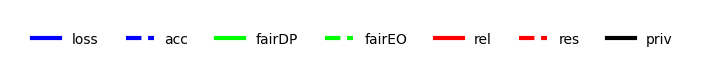
\includegraphics[width=\linewidth]{figs/global_legend.png}
    \end{subfigure}

    % ADULT
    \begin{subfigure}{0.24\textwidth}
        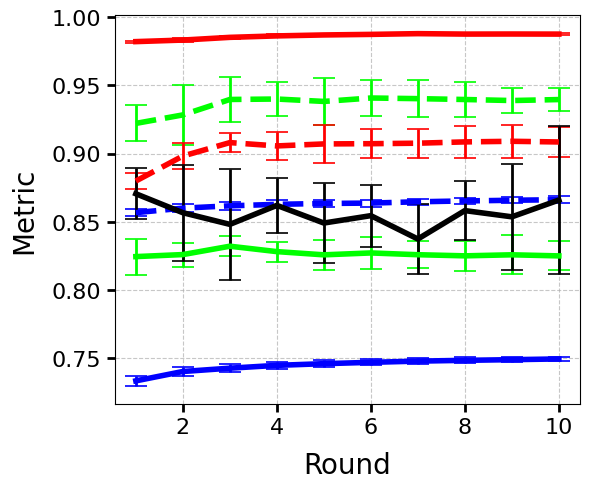
\includegraphics[width=\linewidth]{figs/SE_A_4_I.png}
        \caption{Adult: 4 I}
    \end{subfigure}
    \hfill
    \begin{subfigure}{0.24\textwidth}
        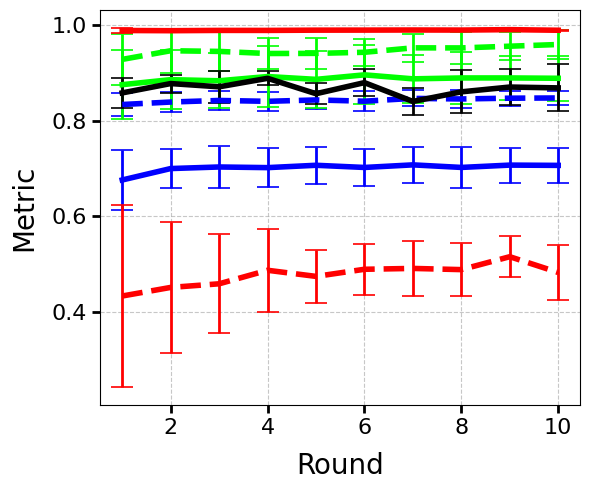
\includegraphics[width=\linewidth]{figs/SE_A_4_N.png}
        \caption{Adult: 4 N}
    \end{subfigure}
    \hfill
    \begin{subfigure}{0.24\textwidth}
        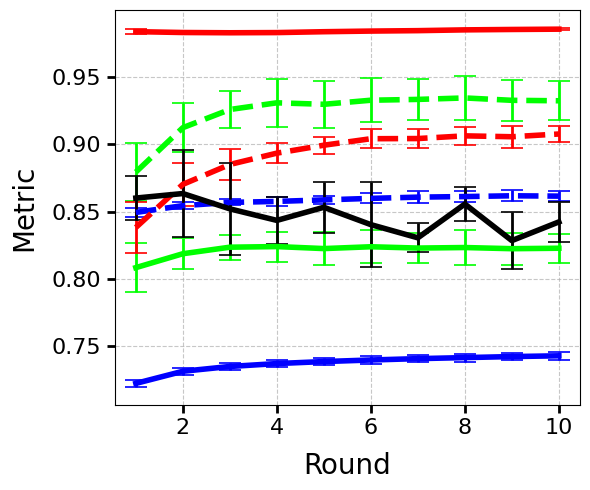
\includegraphics[width=\linewidth]{figs/SE_A_20_I.png}
        \caption{Adult: 20 I}
    \end{subfigure}
    \hfill
    \begin{subfigure}{0.24\textwidth}
        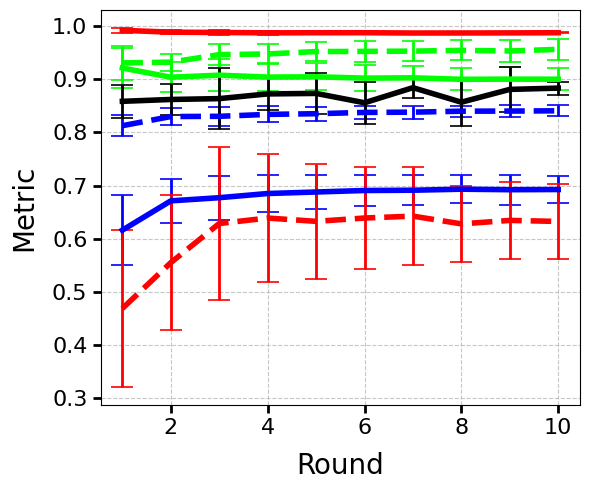
\includegraphics[width=\linewidth]{figs/SE_A_20_N.png}
        \caption{Adult: 20 N}
    \end{subfigure}
    
    % CelebA
    \begin{subfigure}{0.24\textwidth}
        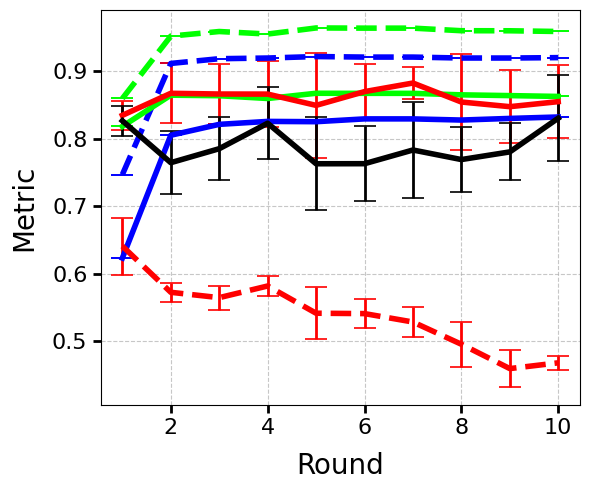
\includegraphics[width=\linewidth]{figs/SE_C_4_I.png}
        \caption{CelebA: 4 I}
    \end{subfigure}
    \hfill
    \begin{subfigure}{0.24\textwidth}
        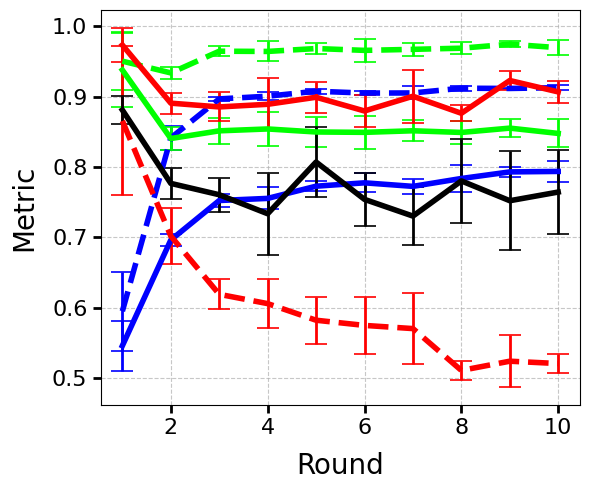
\includegraphics[width=\linewidth]{figs/SE_C_4_N.png}
        \caption{CelebA: 4 N}
    \end{subfigure}
    \hfill
    \begin{subfigure}{0.24\textwidth}
        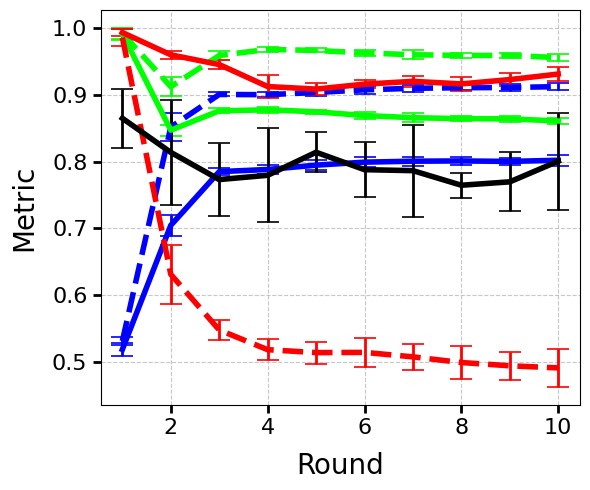
\includegraphics[width=\linewidth]{figs/SE_C_20_I.png}
        \caption{CelebA: 20 I}
    \end{subfigure}
    \hfill
    \begin{subfigure}{0.24\textwidth}
        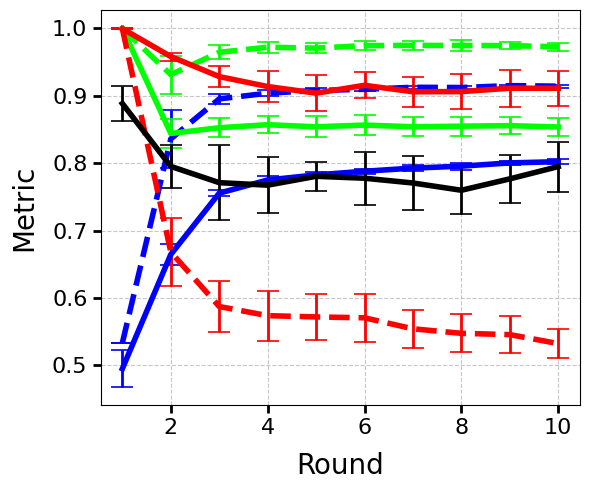
\includegraphics[width=\linewidth]{figs/SE_C_20_N.png}
        \caption{CelebA: 20 N}
    \end{subfigure}
    
    % IMDB
    \begin{subfigure}{0.24\textwidth}
        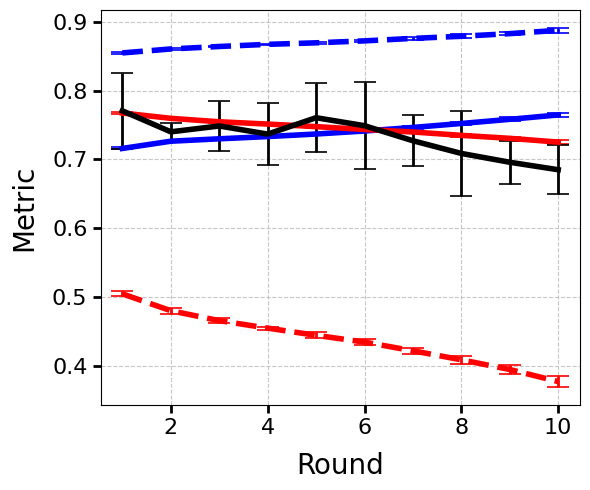
\includegraphics[width=\linewidth]{figs/SE_I_4_I.png}
        \caption{IMDB: 4 I}
    \end{subfigure}
    \hfill
    \begin{subfigure}{0.24\textwidth}
        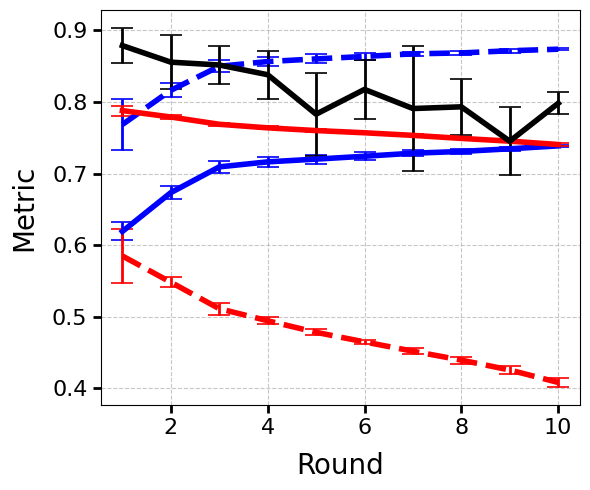
\includegraphics[width=\linewidth]{figs/SE_I_4_N.png}
        \caption{IMDB: 4 N}
    \end{subfigure}
    \hfill 
    \begin{subfigure}{0.24\textwidth}
        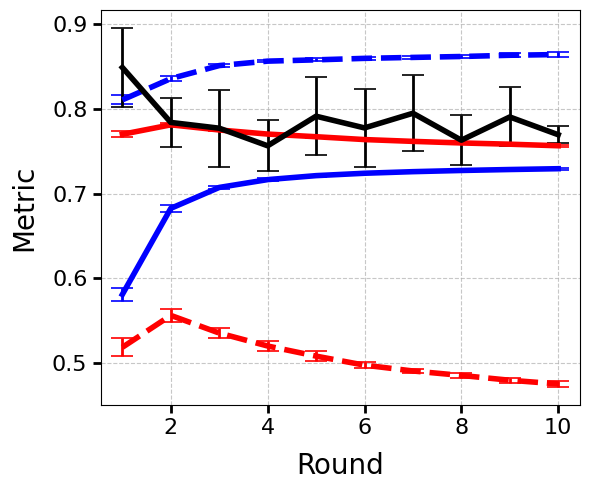
\includegraphics[width=\linewidth]{figs/SE_I_20_I.png}
        \caption{IMDB: 20 I}
    \end{subfigure}
    \hfill
    \begin{subfigure}{0.24\textwidth}
        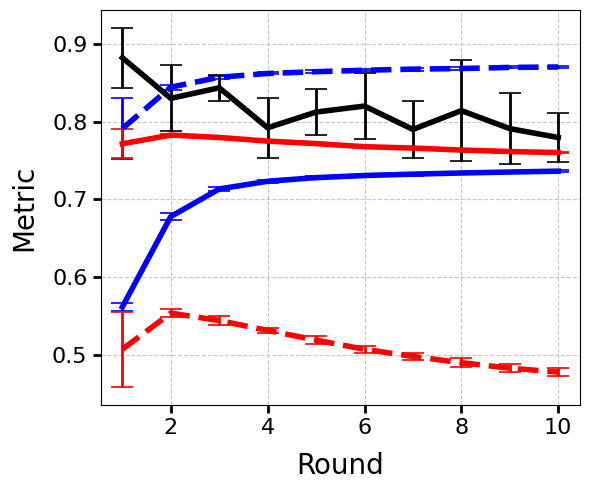
\includegraphics[width=\linewidth]{figs/SE_I_20_N.png}
        \caption{IMDB: 20 N}
    \end{subfigure}
    
    \caption{Score evolution of the model as the training progresses.}
    \label{fig:score_evol}
\end{figure}

First we study how the model's various scores change during the training. It is clear that $\mathtt{loss}$ improves, as it is directly optimized. As a direct consequence, $\mathtt{acc}$ also improves. On the other hand, the metrics capturing trustworthiness are not explicitly considered, hence, their evolution is not necessarily improving. This is visualized in Fig.~\ref{fig:score_evol}. Here, one can see widely different trends across datasets. On the ADULT dataset the scores are largely stable under IID partitioning; the non-IID panels show only modest movement, chiefly a mild upward drift in resilience together with small changes in loss. This relative stability follows from the limited evolution of the global model between rounds 2 and 10: the comparatively simple tabular task is essentially learned in the first round, leaving little room for fluctuation across the performance or trustworthiness dimensions.

In contrast, the trajectories on CelebA differ drastically. As expected, the performance score steadily increases as the global model is explicitly optimized for it. Meanwhile, both fairness metrics ($\mathtt{fairDP}$ and $\mathtt{fairEO}$) remain highly stationary near the top of the scale. However, because the standard federated training process does not explicitly optimize for robustness or privacy, these properties deteriorate. After the first round, resilience and privacy suffer steep or steady declines, while reliability drops once between rounds 1 and 2 and then plateaus. This visually demonstrates that standard performance optimization can actively harm these specific trustworthy dimensions if left unchecked.

Finally, on the IMDB dataset (where the fairness scores are omitted), changes in reliability ($0.6 < \mathtt{rel} < 0.8$) are considerably more moderate compared to resilience ($0.35 < \mathtt{res} < 0.6$), and unlike CelebA, neither robustness metric exhibits a clear, monotonic trend. Privacy, however, does show a clear and steady degradation as the training rounds progress. Ultimately, these results show that trustworthiness metrics can behave radically differently across distinct settings, and even closely related metrics can paint varying pictures of the same model. While we strongly advocate for deeper research into the dynamics of global model trustworthiness over time, the primary focus of this paper is evaluating individual client contributions, which we explore next.

\subsubsection*{Trustworthy Client Scores}

\begin{figure}[!b]
    \centering
    
    \begin{subfigure}{0.9\linewidth}
        \centering
        
\includegraphics[width=\linewidth]{figs/S_legend.png}
    \end{subfigure}
    
    % ADULT - 4 Clients
    \begin{subfigure}{0.24\textwidth}
        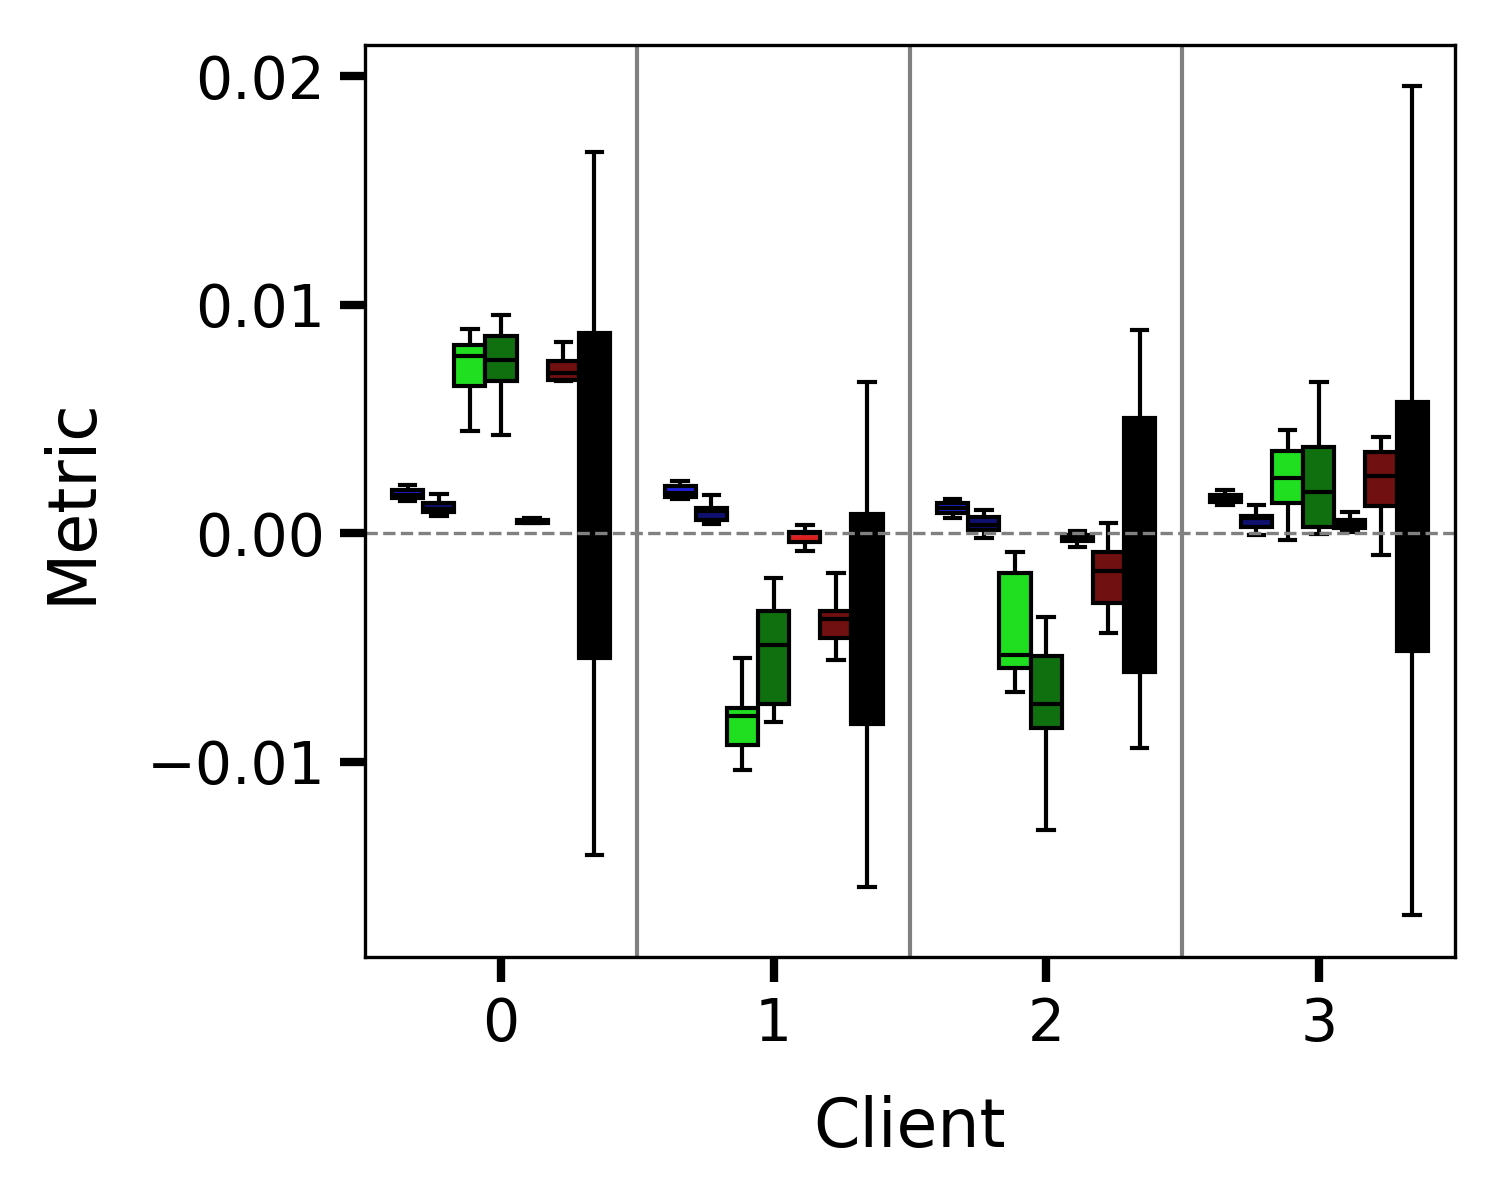
\includegraphics[width=\linewidth]{figs/S_A_4_I_l1o.png}
        \caption{Adult: 4 I / LOO}
    \end{subfigure}
    \hfill
    \begin{subfigure}{0.24\textwidth}
        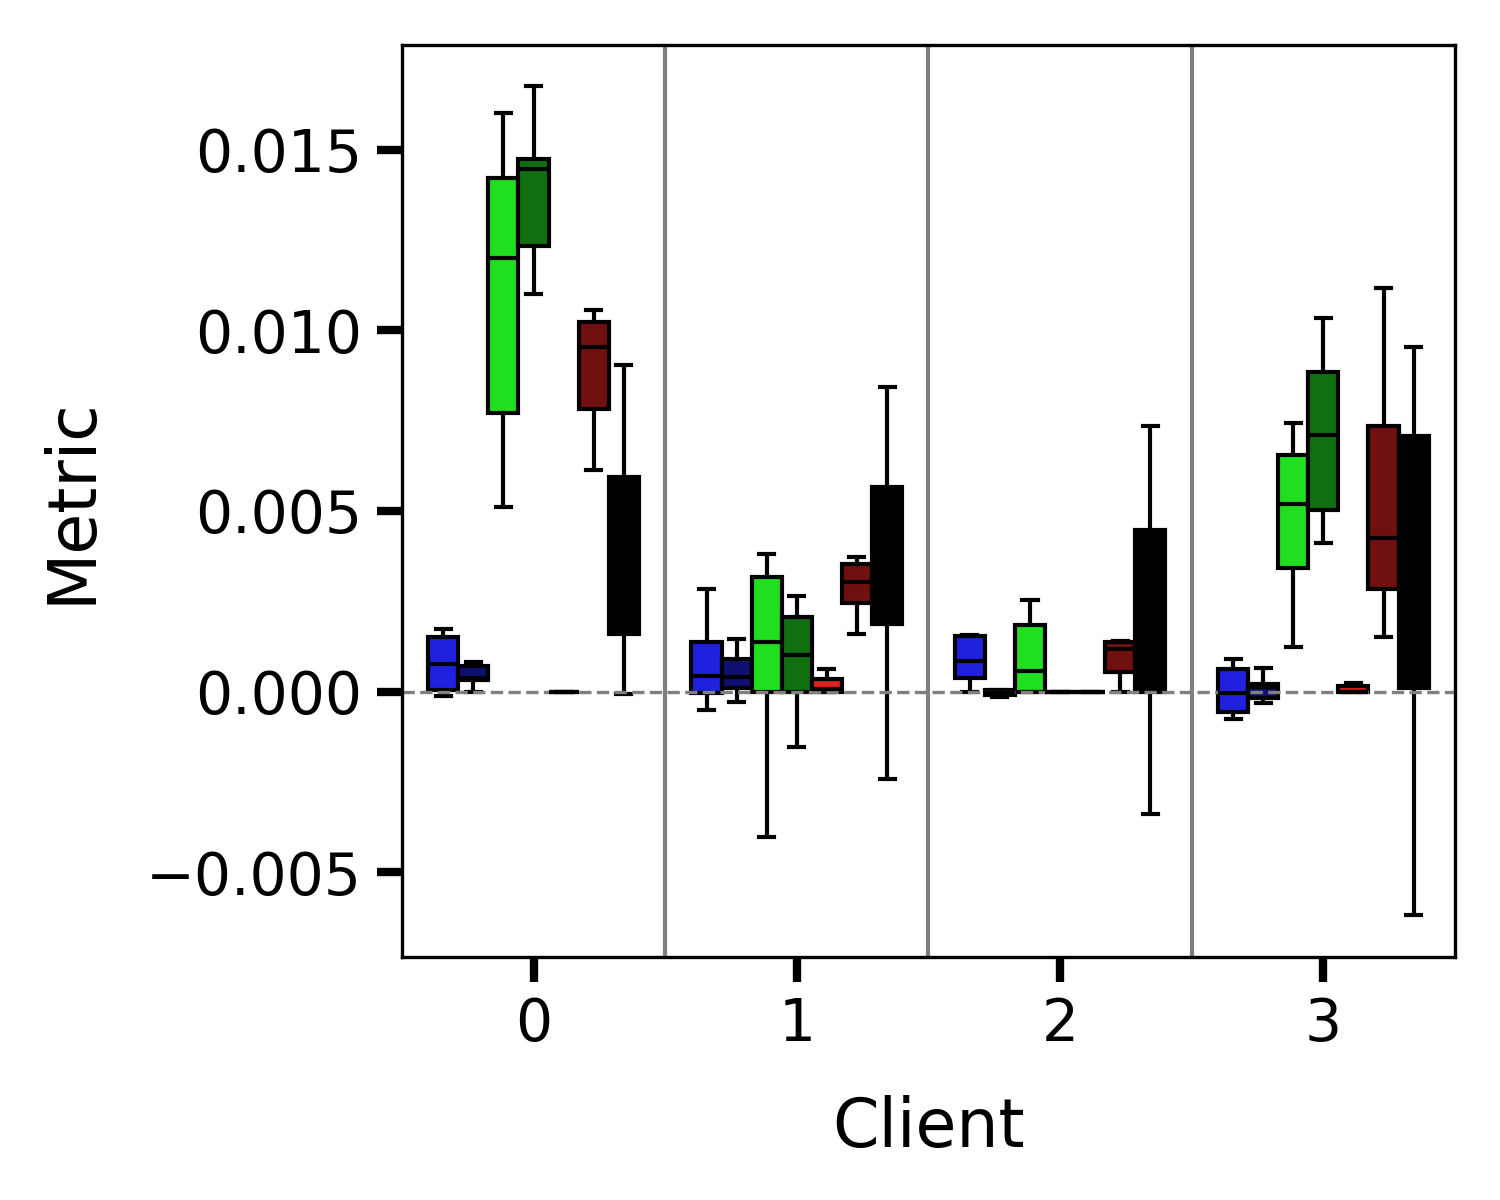
\includegraphics[width=\linewidth]{figs/S_A_4_I_gtg.png}
        \caption{Adult: 4 I / GTG}
    \end{subfigure}
    \hfill
    \begin{subfigure}{0.24\textwidth}
        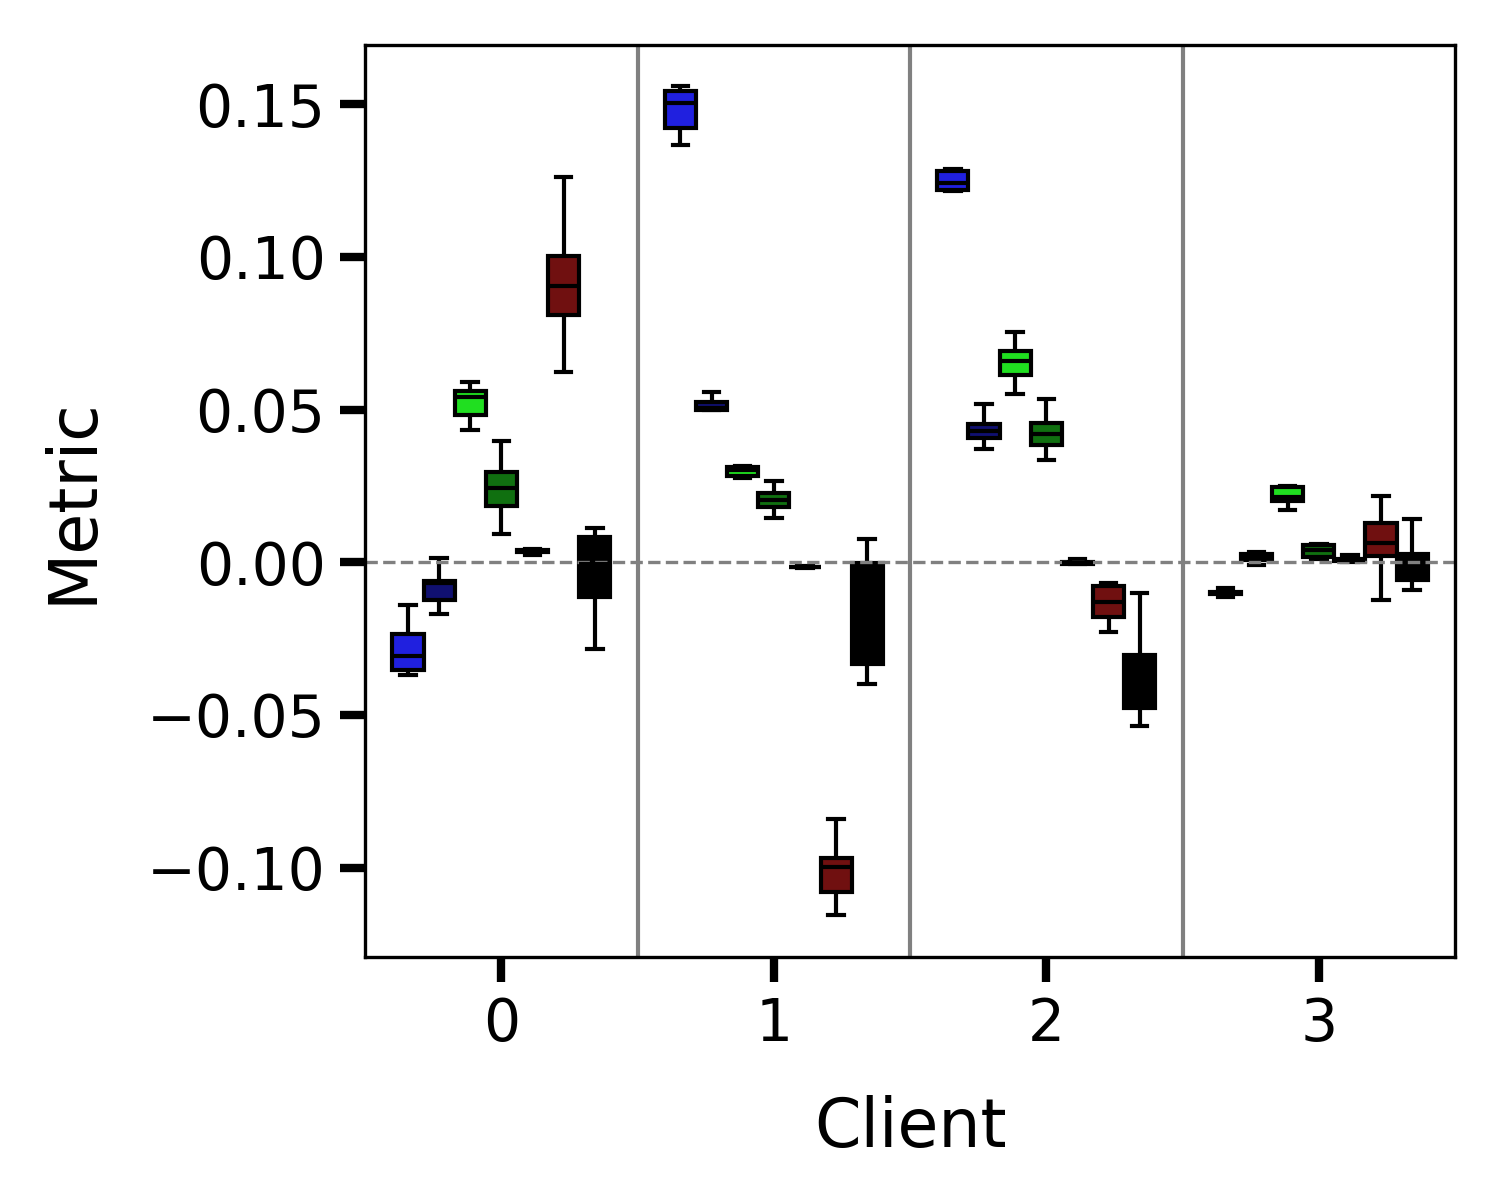
\includegraphics[width=\linewidth]{figs/S_A_4_N_l1o.png}
        \caption{Adult: 4 N / LOO}
    \end{subfigure}
    \hfill
    \begin{subfigure}{0.24\textwidth}
        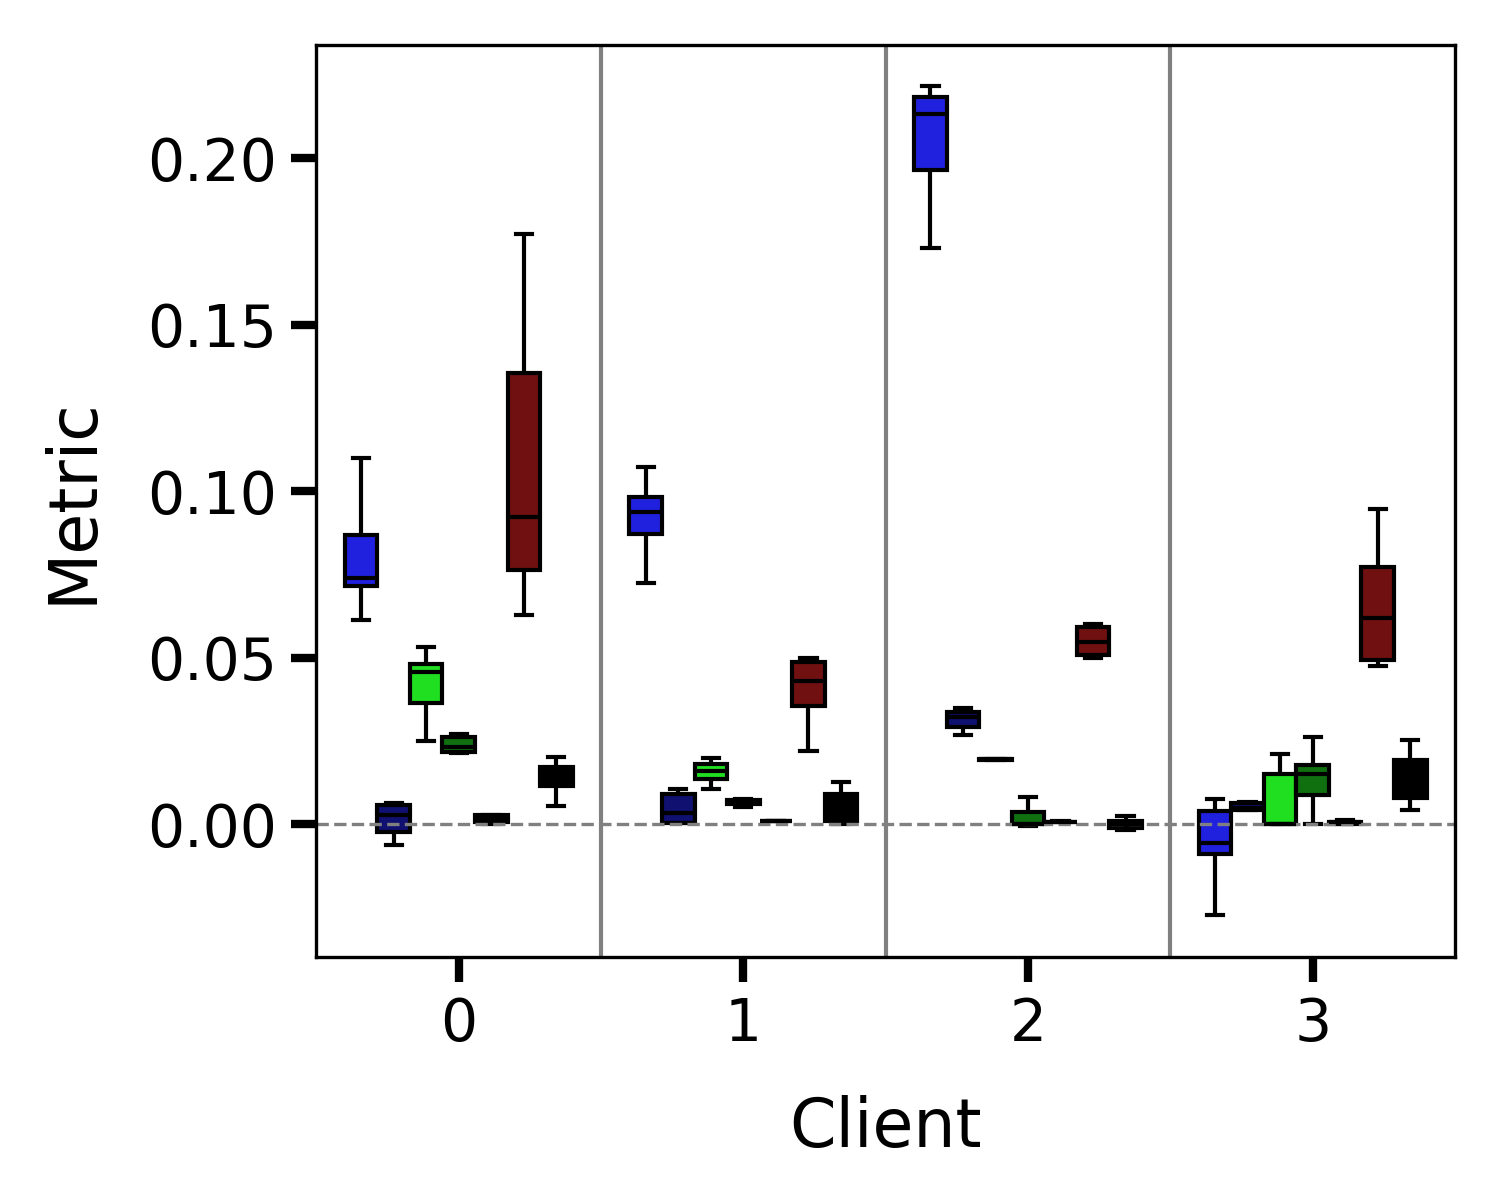
\includegraphics[width=\linewidth]{figs/S_A_4_N_gtg.png}
        \caption{Adult: 4 N / GTG}
    \end{subfigure}

    % CelebA - 4 Clients
    \begin{subfigure}{0.24\textwidth}
        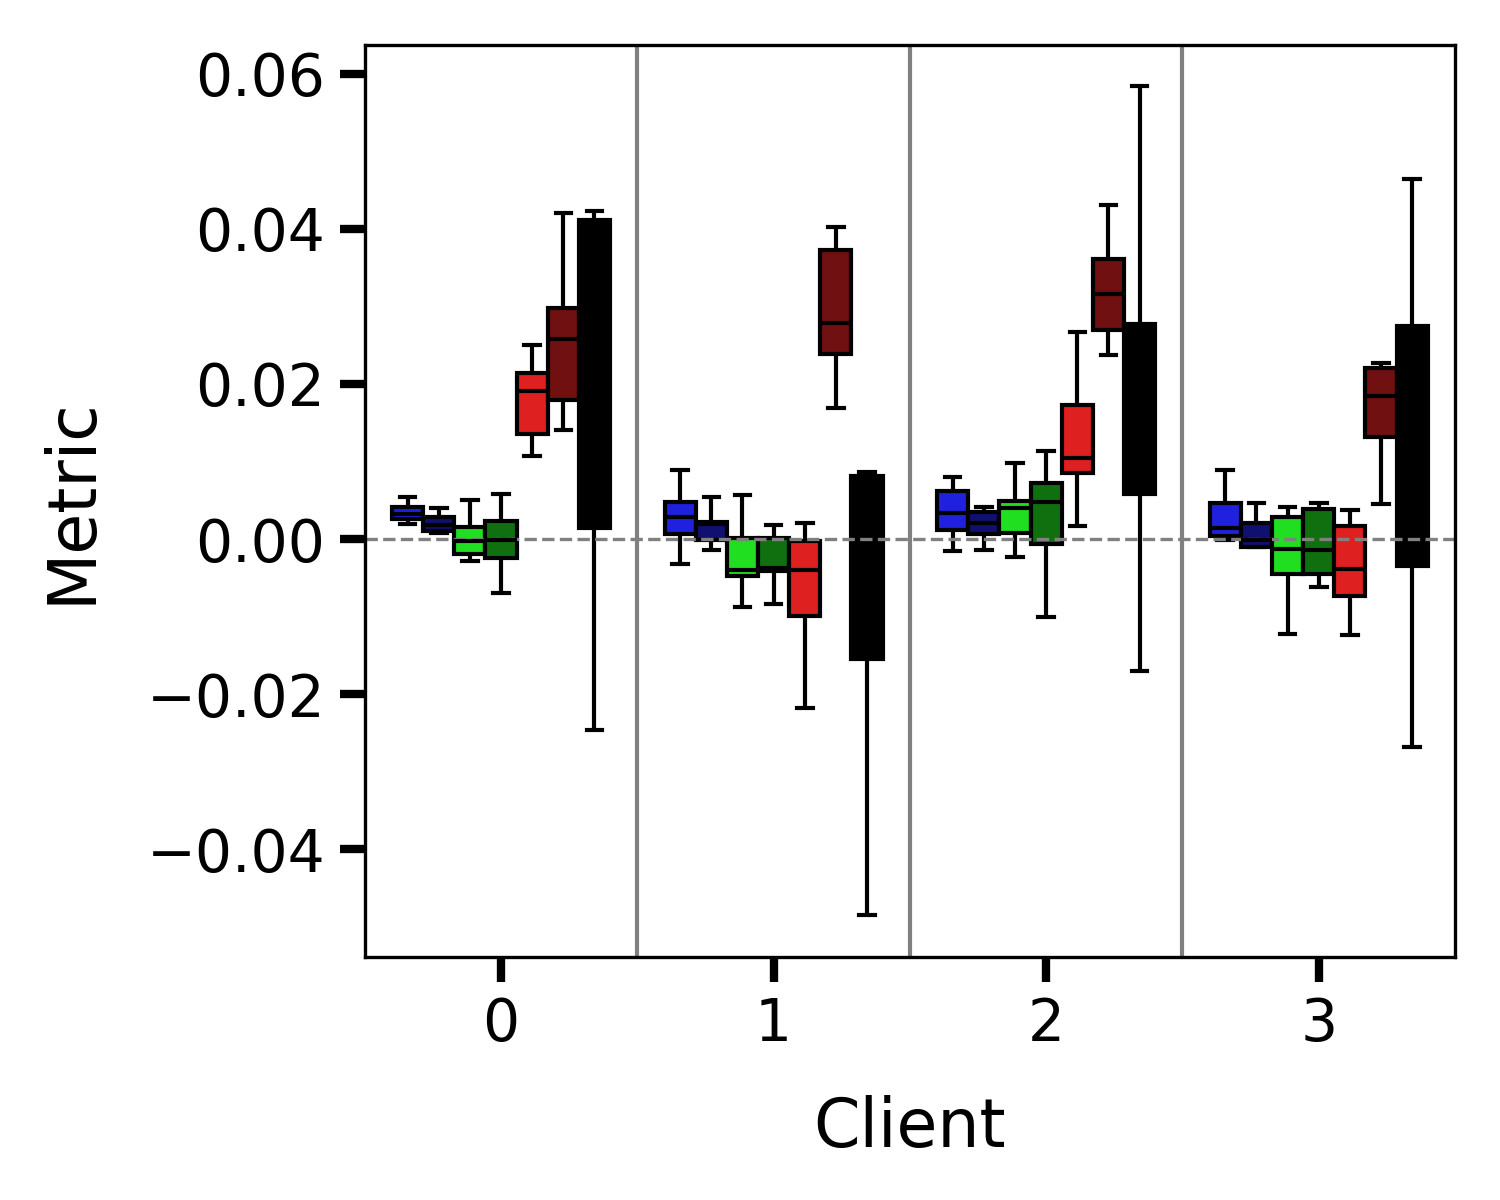
\includegraphics[width=\linewidth]{figs/S_C_4_I_l1o.png}
        \caption{CelebA: 4 I / LOO}
    \end{subfigure}
    \hfill
    \begin{subfigure}{0.24\textwidth}
        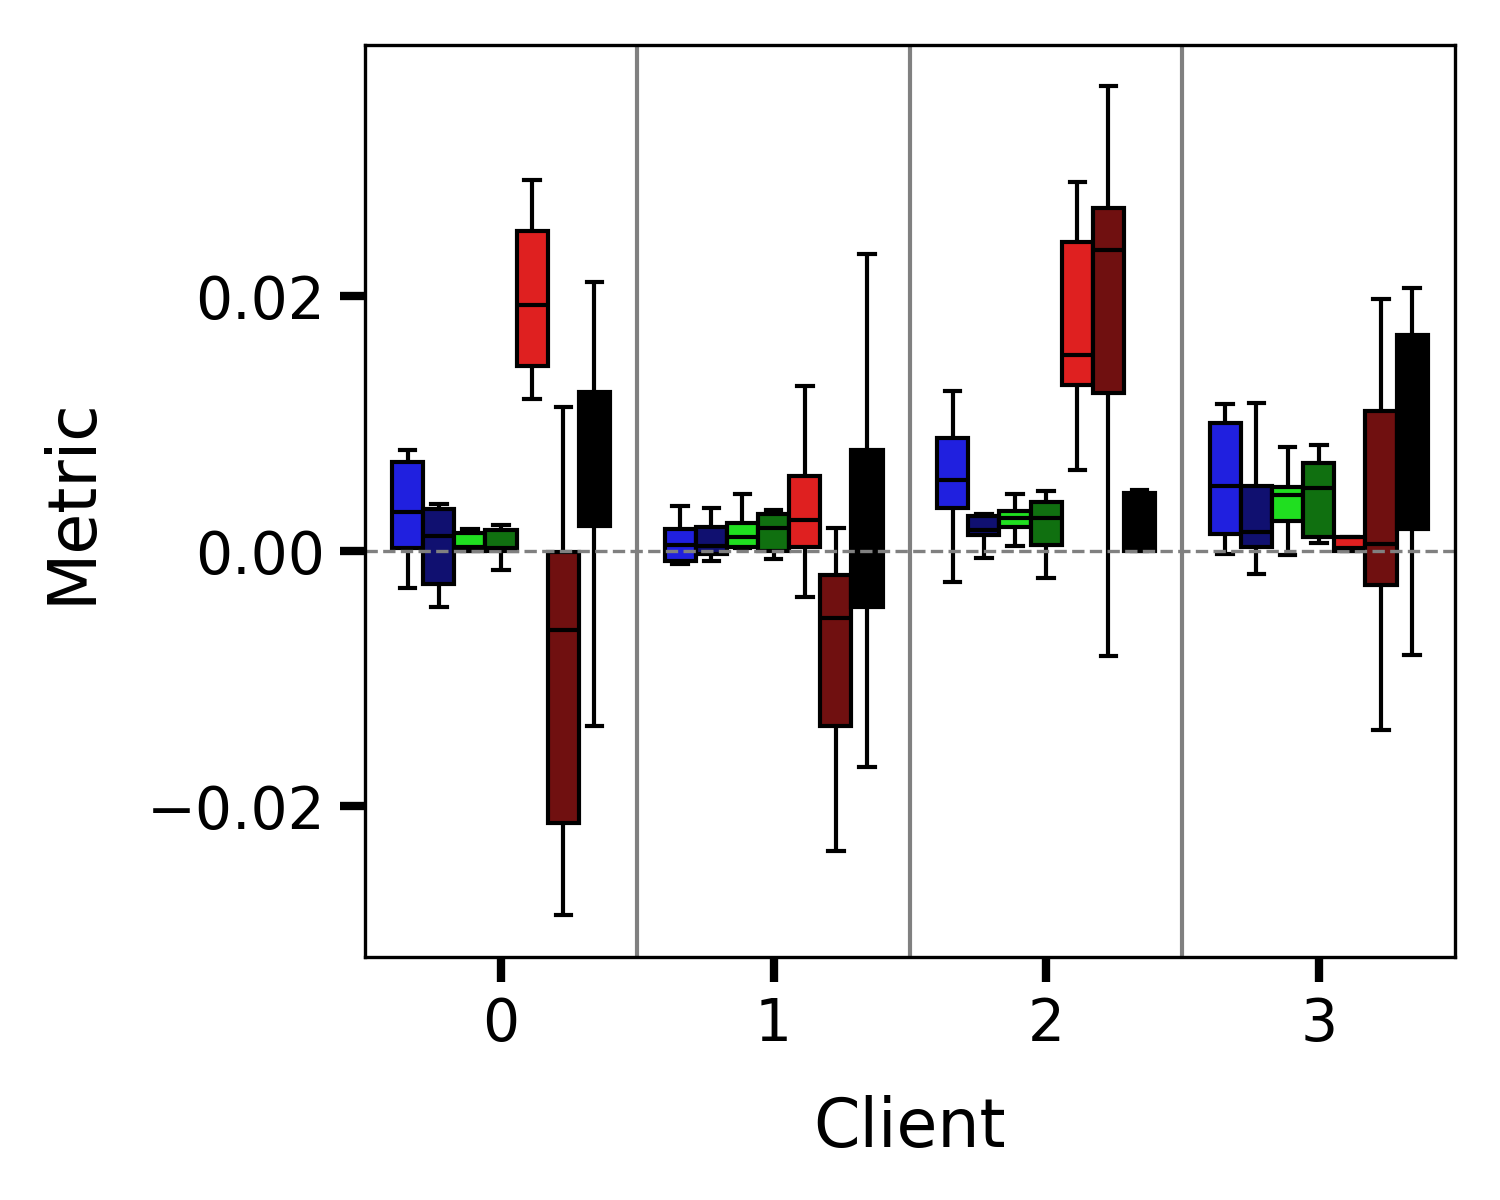
\includegraphics[width=\linewidth]{figs/S_C_4_I_gtg.png}
        \caption{CelebA: 4 I / GTG}
    \end{subfigure}
    \hfill
    \begin{subfigure}{0.24\textwidth}
        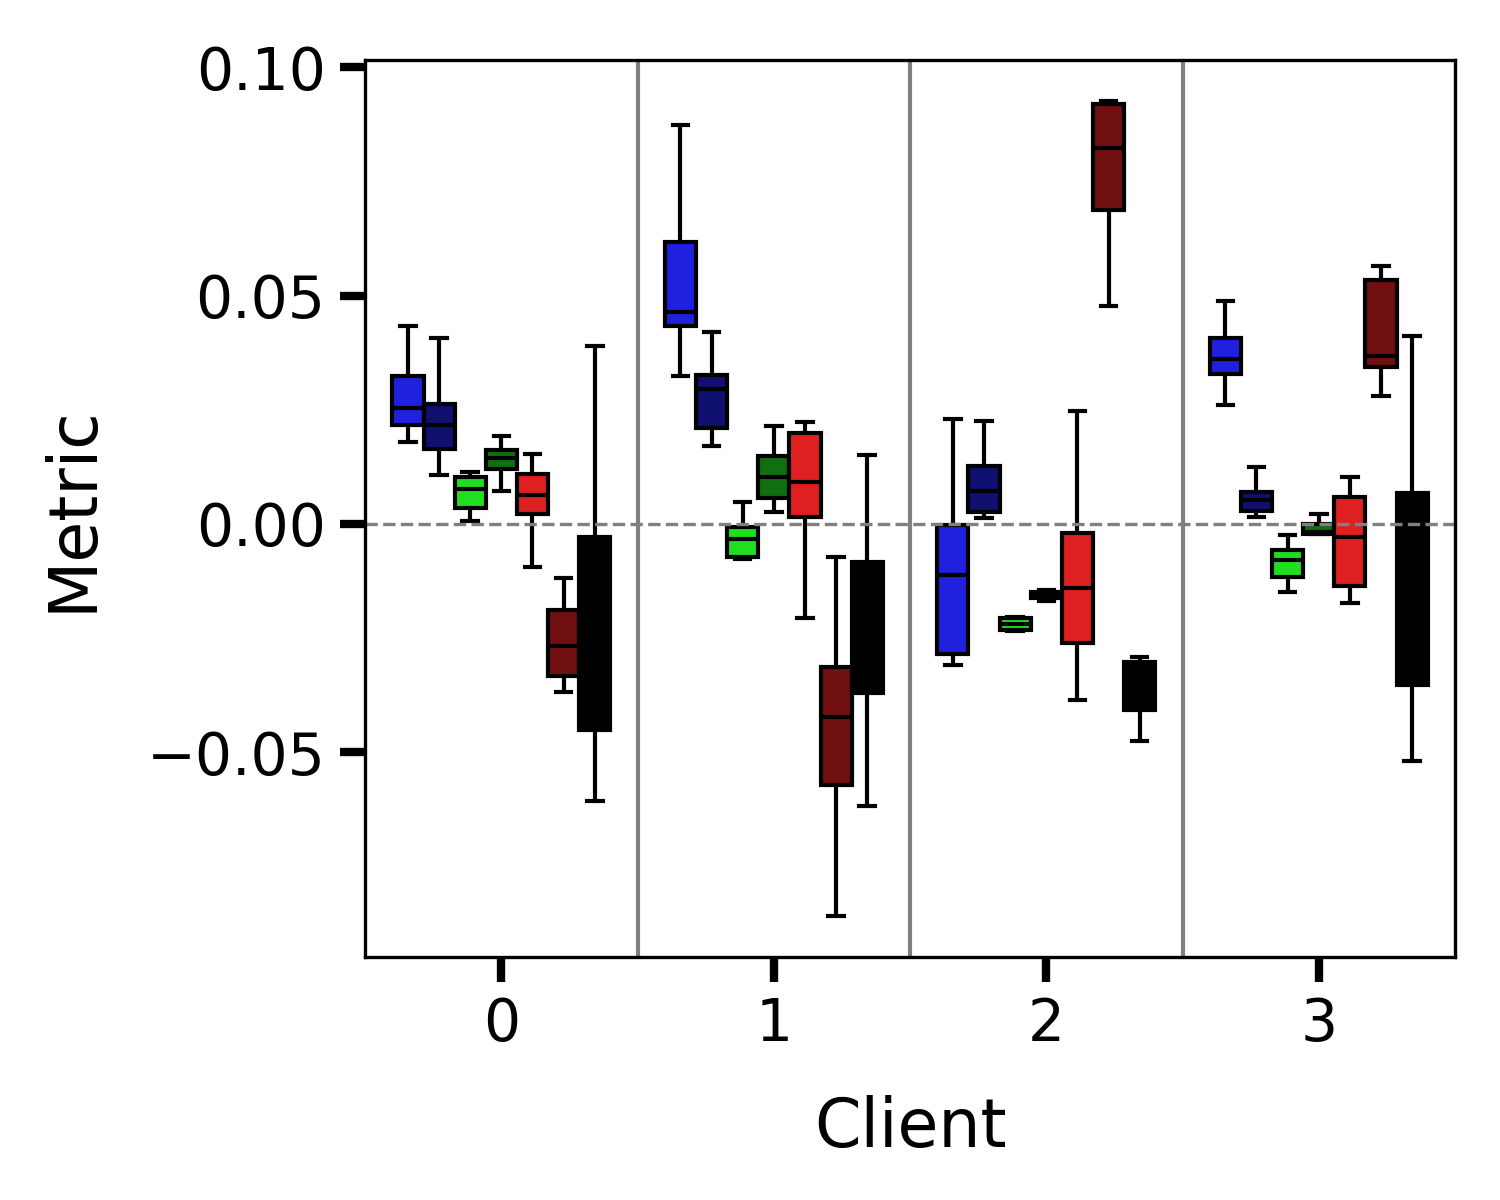
\includegraphics[width=\linewidth]{figs/S_C_4_N_l1o.png}
        \caption{CelebA: 4 N / LOO}
    \end{subfigure}
    \hfill
    \begin{subfigure}{0.24\textwidth}
        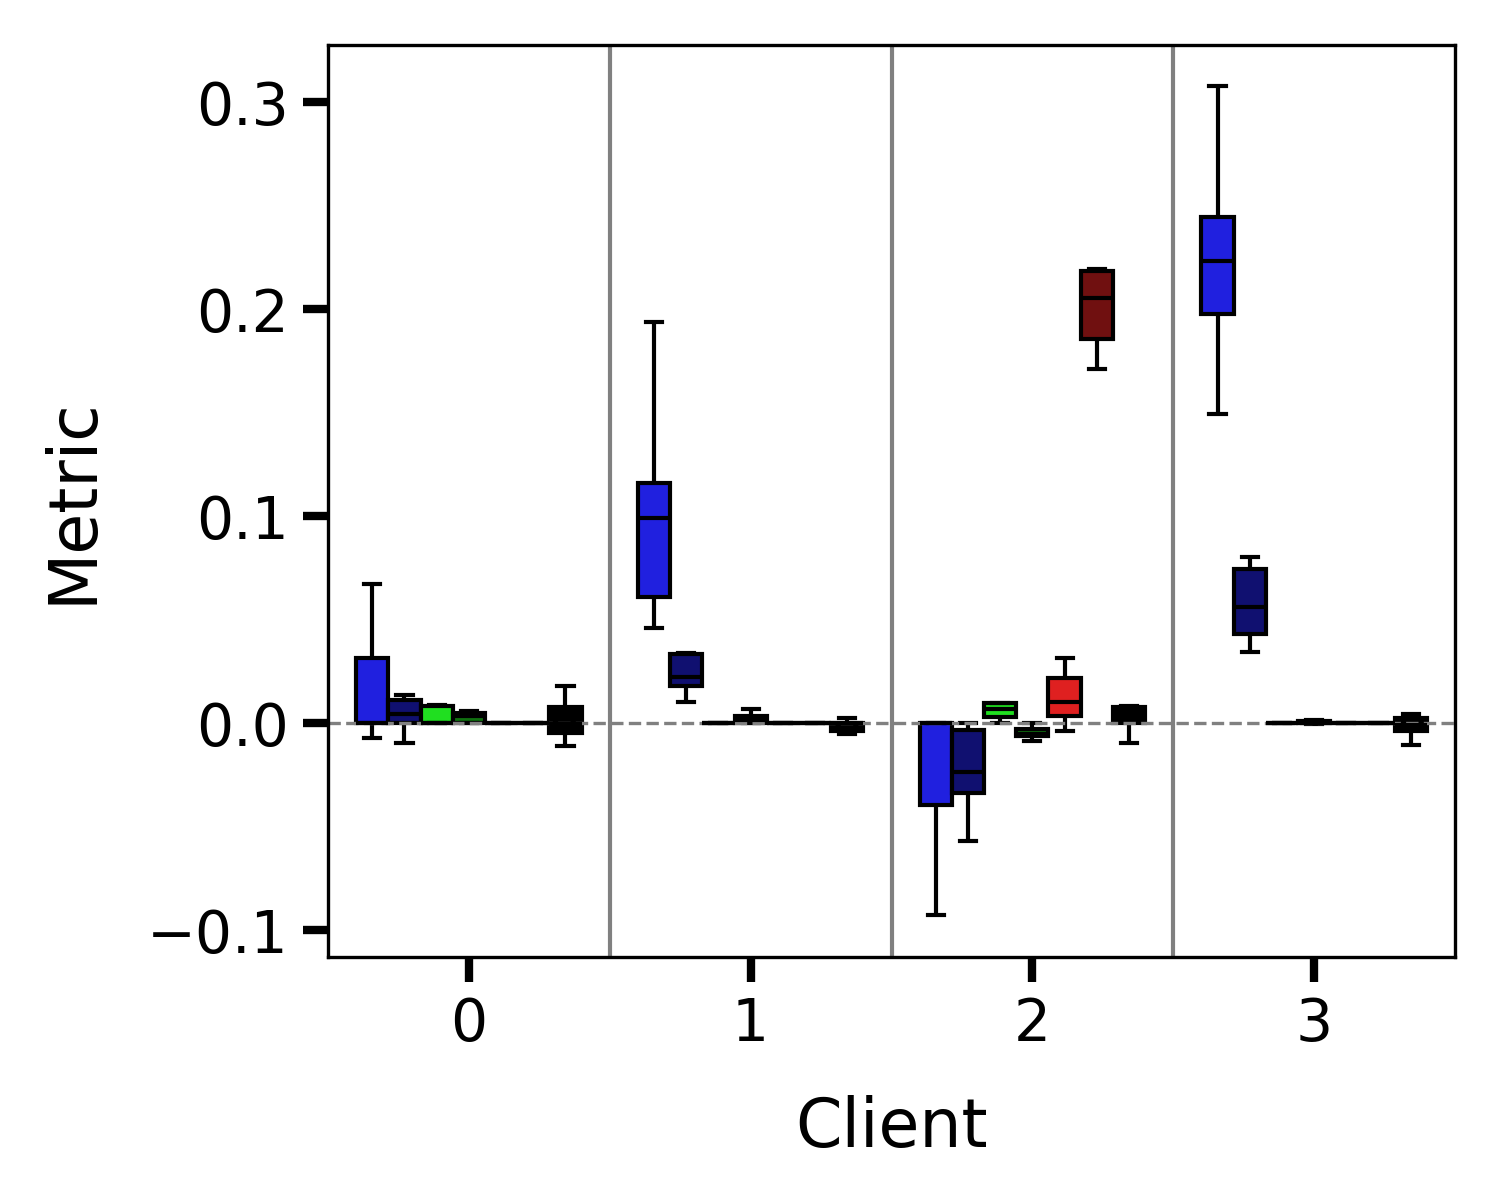
\includegraphics[width=\linewidth]{figs/S_C_4_N_gtg.png}
        \caption{CelebA: 4 N / GTG}
    \end{subfigure}

    % IMDB - 4 Clients
    \begin{subfigure}{0.24\textwidth}
        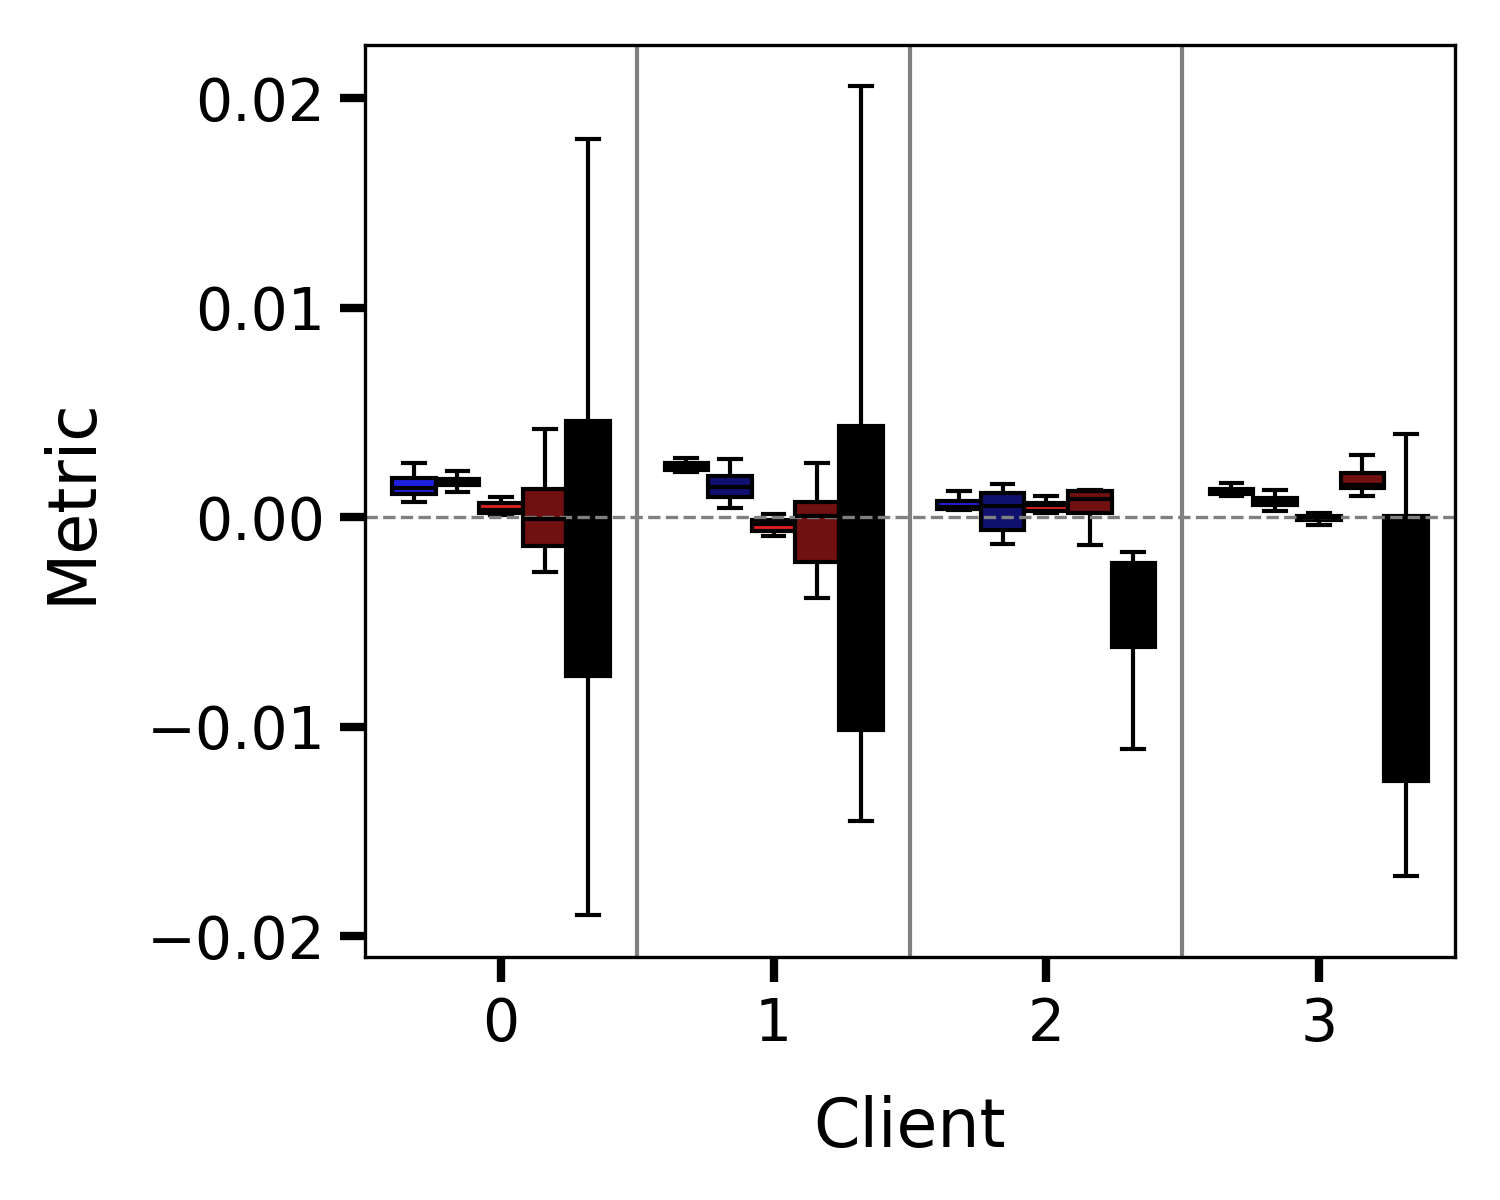
\includegraphics[width=\linewidth]{figs/S_I_4_I_l1o.png}
        \caption{IMDB: 4 I / LOO}
    \end{subfigure}
    \hfill
    \begin{subfigure}{0.24\textwidth}
        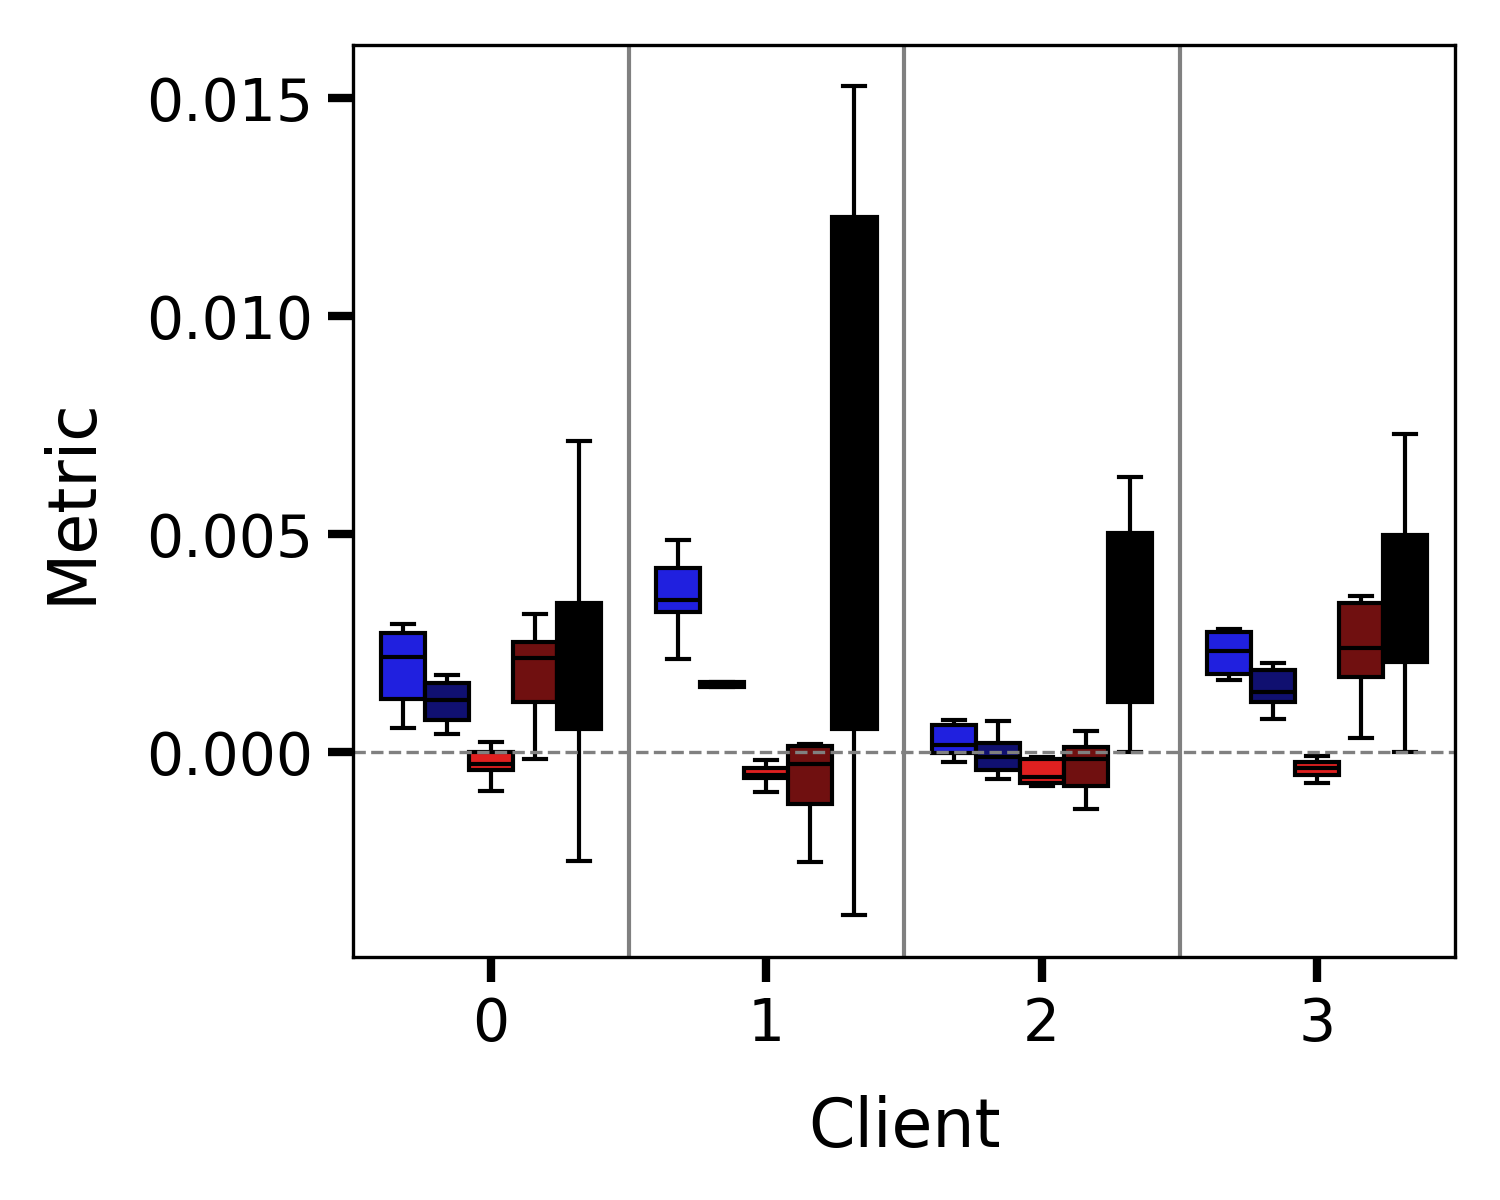
\includegraphics[width=\linewidth]{figs/S_I_4_I_gtg.png}
        \caption{IMDB: 4 I / GTG}
    \end{subfigure}
    \hfill
    \begin{subfigure}{0.24\textwidth}
        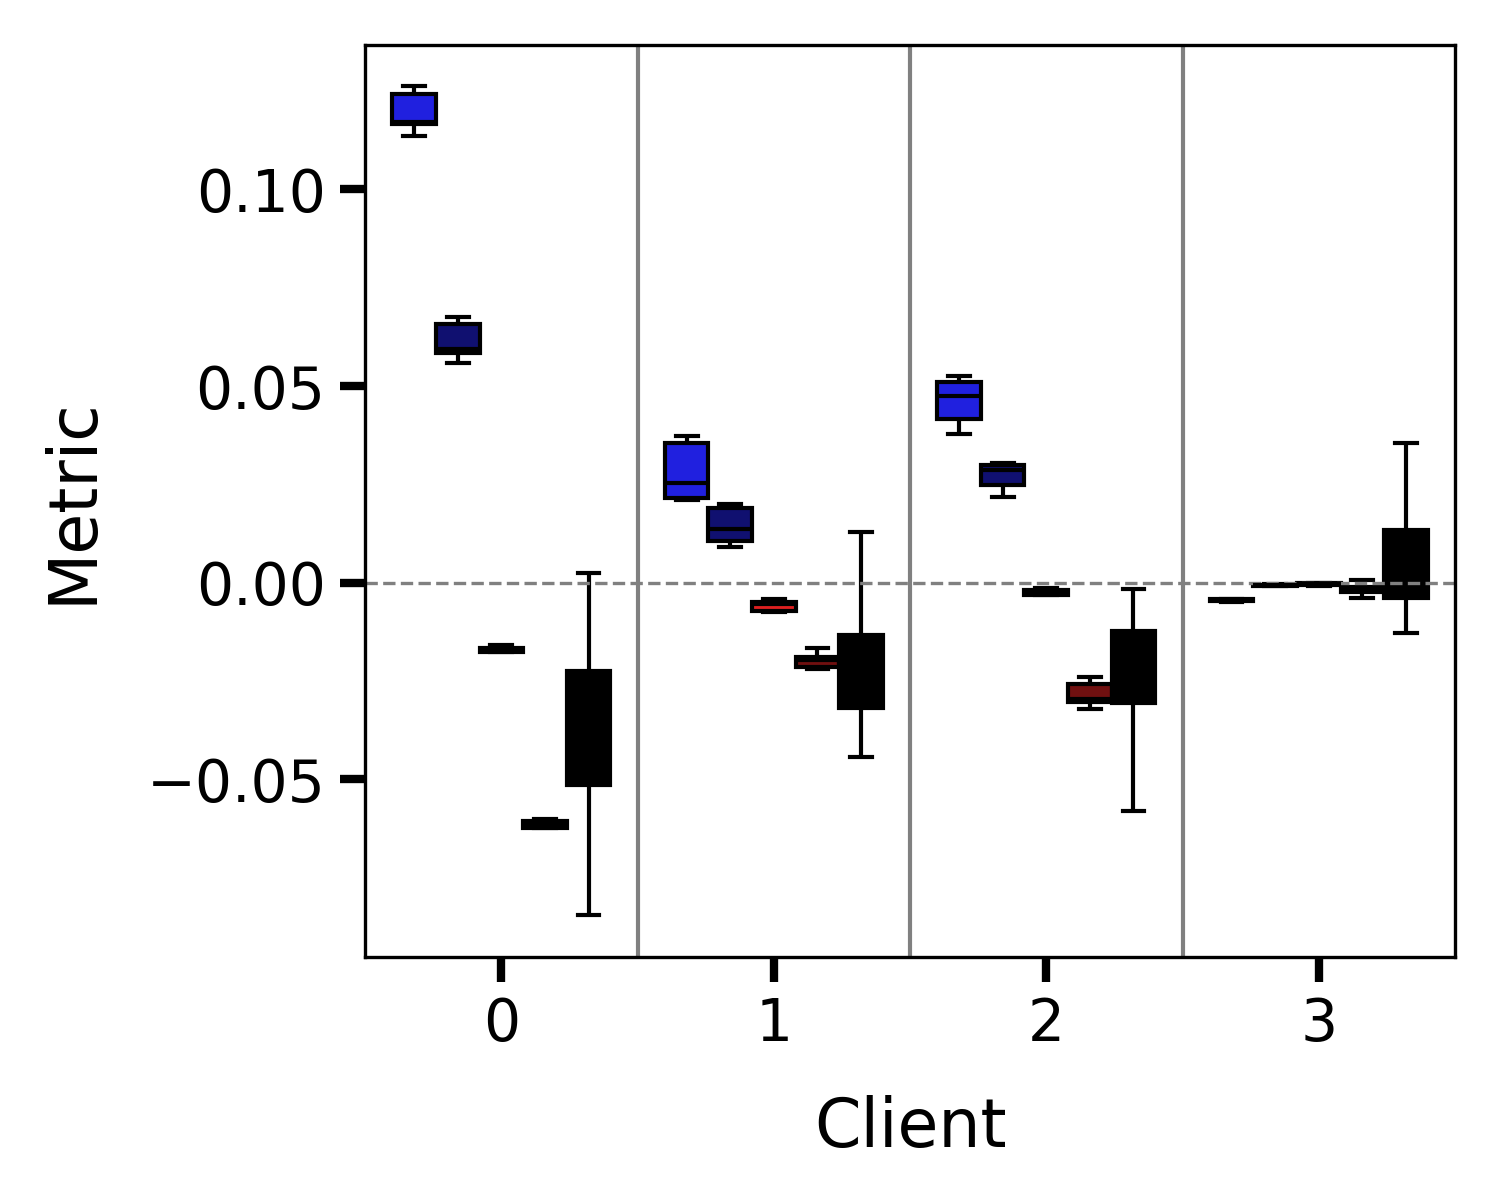
\includegraphics[width=\linewidth]{figs/S_I_4_N_l1o.png}
        \caption{IMDB: 4 N / LOO}
    \end{subfigure}
    \hfill
    \begin{subfigure}{0.24\textwidth}
        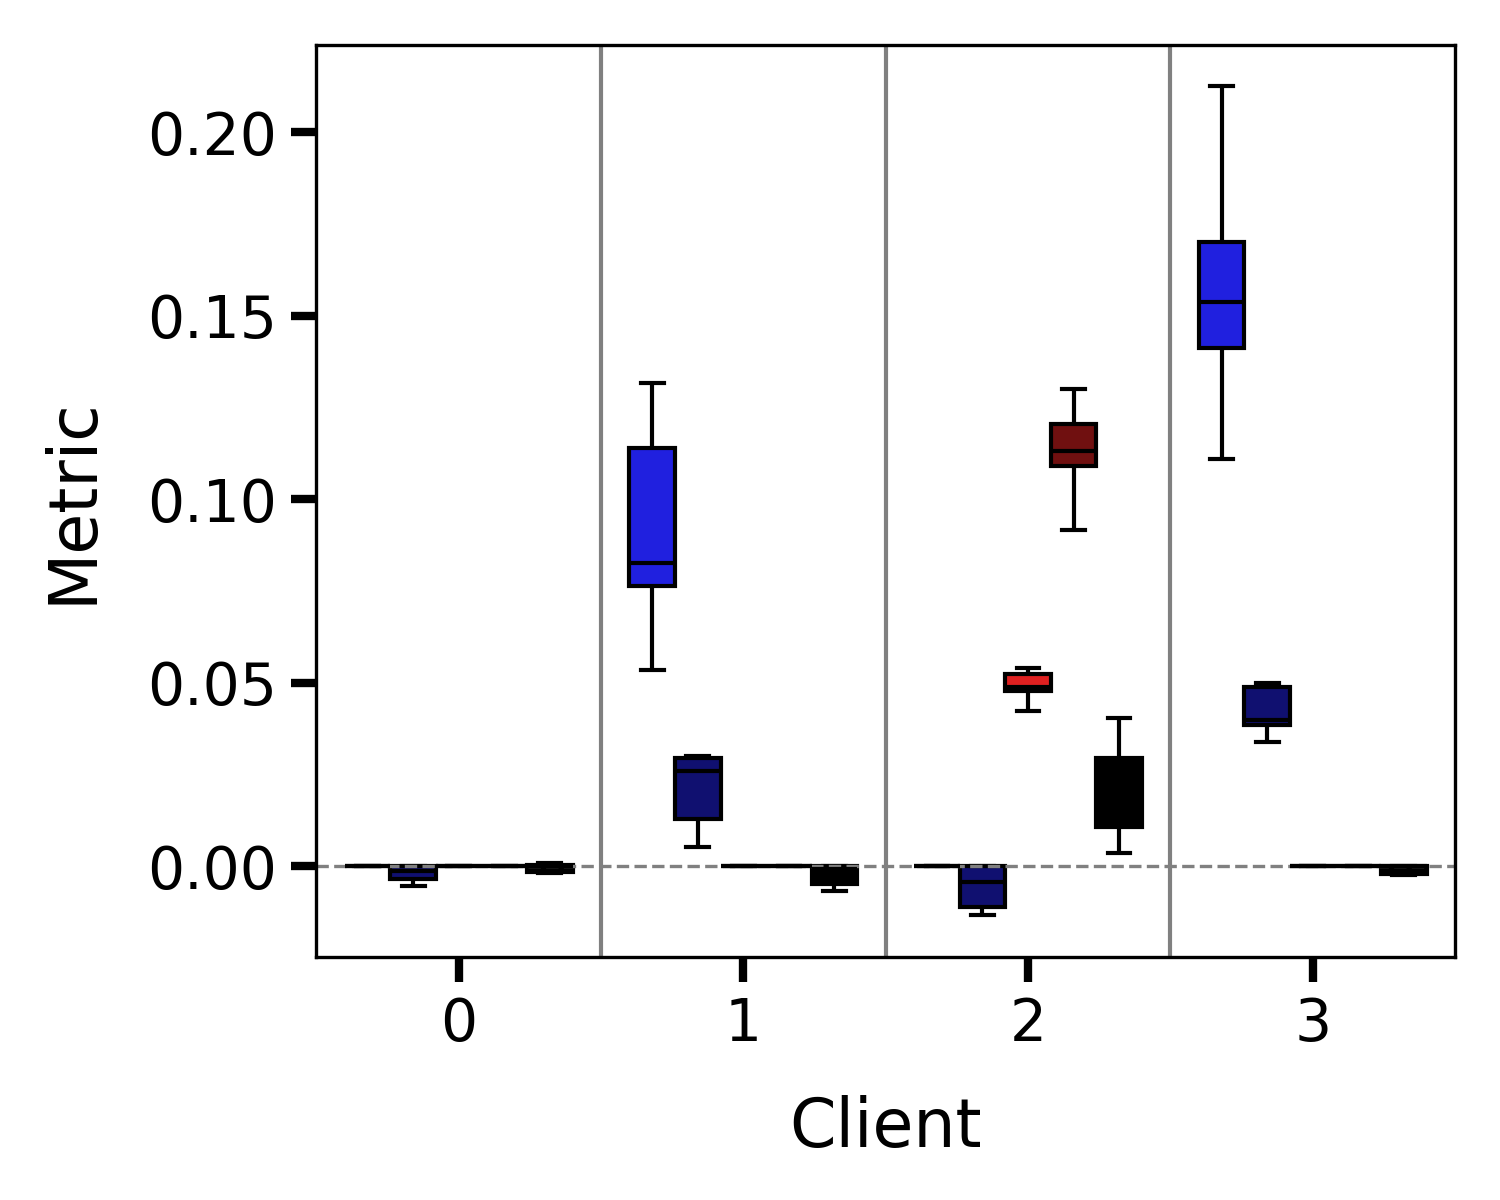
\includegraphics[width=\linewidth]{figs/S_I_4_N_gtg.png}
        \caption{IMDB: 4 N / GTG}
    \end{subfigure}
    
    \caption{Computed contribution scores (accumulated across rounds) for the $K=4$ client scenario; I and N denote IID and non-IID, respectively.}
    \label{fig:scores_4_clients}
\end{figure}

Next, based on the global model's performance, we allocate individual trustworthiness contribution scores to the clients. While the global model exhibits a single trajectory, this is merely the aggregated result of the clients' individual contributions, which can drastically differ from one another. We present the obtained scores for $K=4$ in Fig.~\ref{fig:scores_4_clients} ($K=20$ is in the Appendix). For the per-client visual analysis we focus on the $K=4$ scenario, where the discrete individual behaviors are easiest to untangle. 

Some consistent patterns emerge across all three datasets and contribution evaluation schemes. Notably, the evaluation method plays a large role in the distribution: while GTG-Shapley tends to allocate mostly positive scores with tighter bounds (due to its permutation averaging), the LOO evaluations frequently reveal stark negative contributions across all metrics. Crucially, several "dominant" clients appear that substantially improve the global model according to one specific metric, while simultaneously offering no benefit (or actively proving harmful) in another. This is where the complex trade-offs between performance, fairness, robustness, and privacy become the most visible. This empirically demonstrates that trustworthy behavior cannot be achieved by optimizing for or valuing clients based on global accuracy alone. This contribution analysis also reveals that trustworthiness in federated systems is inherently client-dependent: specific clients consistently exert positive effects on a particular dimension, while others consistently degrade it. This multidimensional evaluation provides not only a vital diagnostic insight into the federation's health but also establishes a mathematical basis for governance mechanisms that can actively steer federated AI systems toward a more trustworthy operation. 

\subsubsection*{Trustworthy Score Evolution}

\begin{table}[!b]
    \centering
    \resizebox{\linewidth}{!}{%
    \begin{tabular}{ccc||c|c|c|c|c|c|c}
        \multicolumn{3}{c||}{\textbf{Setting}}
        & \textbf{$\mathtt{acc}$}
        & \textbf{$\mathtt{loss}$}
        & \textbf{$\mathtt{fairDP}$}
        & \textbf{$\mathtt{fairEO}$}
        & \textbf{$\mathtt{rel}$}
        & \textbf{$\mathtt{res}$}
        & \textbf{$\mathtt{priv}$} \\
        \hline\hline
        \multirow{4}{*}{\rotatebox{90}{ADULT}} & \multirow{2}{*}{4} & I & 5.7$e$-4$\pm$1.8$e$-4 & 1.4$e$-3$\pm$3.3$e$-4 & 4.0$e$-3$\pm$2.4$e$-4 & 3.0$e$-3$\pm$1.0$e$-3 & 1.8$e$-4$\pm$4.9$e$-5 & 2.7$e$-3$\pm$1.0$e$-3 & 7.2$e$-3$\pm$1.0$e$-3 \\
        && N & 6.3$e$-3$\pm$4.3$e$-3 & 2.4$e$-2$\pm$1.3$e$-2 & 6.4$e$-3$\pm$3.7$e$-3 & 5.5$e$-3$\pm$2.6$e$-3 & 5.5$e$-4$\pm$3.0$e$-4 & 2.6$e$-2$\pm$2.2$e$-2 & 9.6$e$-3$\pm$1.8$e$-3 \\
        \cline{2-10}
        & \multirow{2}{*}{20} & I & 1.0$e$-4$\pm$3.4$e$-5 & 2.1$e$-4$\pm$4.2$e$-5 & 3.9$e$-4$\pm$1.0$e$-4 & 8.3$e$-4$\pm$1.9$e$-4 & 1.1$e$-5$\pm$1.1$e$-5 & 7.2$e$-4$\pm$1.1$e$-4 & 9.2$e$-4$\pm$2.4$e$-4 \\
        && N & 3.3$e$-3$\pm$8.2$e$-4 & 1.2$e$-2$\pm$1.3$e$-3 & 1.8$e$-3$\pm$1.4$e$-3 & 3.2$e$-3$\pm$1.2$e$-3 & 1.1$e$-4$\pm$6.0$e$-5 & 3.5$e$-3$\pm$2.6$e$-3 & 1.9$e$-3$\pm$5.5$e$-4 \\
        \hline
        \multirow{4}{*}{\rotatebox{90}{CelebA}} & \multirow{2}{*}{4} & I & 7.9$e$-3$\pm$2.0$e$-3 & 1.6$e$-2$\pm$4.3$e$-3 & 4.0$e$-3$\pm$5.7$e$-4 & 5.7$e$-3$\pm$9.0$e$-4 & 1.4$e$-2$\pm$3.2$e$-3 & 2.2$e$-2$\pm$2.6$e$-3 & 1.6$e$-2$\pm$1.3$e$-3 \\
        && N & 2.9$e$-2$\pm$3.4$e$-3 & 6.0$e$-2$\pm$3.2$e$-2 & 5.4$e$-3$\pm$1.3$e$-3 & 4.7$e$-3$\pm$5.0$e$-4 & 5.2$e$-3$\pm$5.9$e$-4 & 1.1$e$-2$\pm$4.3$e$-3 & 1.3$e$-2$\pm$3.2$e$-3 \\
        \cline{2-10}
        & \multirow{2}{*}{20} & I & 2.7$e$-3$\pm$4.6$e$-4 & 3.4$e$-3$\pm$9.3$e$-4 & 4.4$e$-4$\pm$1.2$e$-4 & 8.2$e$-4$\pm$1.2$e$-4 & 2.0$e$-3$\pm$5.6$e$-4 & 5.4$e$-3$\pm$6.1$e$-4 & 7.0$e$-3$\pm$4.5$e$-4 \\
        && N & 7.2$e$-3$\pm$1.5$e$-3 & 1.2$e$-2$\pm$3.8$e$-3 & 6.7$e$-4$\pm$1.7$e$-4 & 4.1$e$-4$\pm$1.5$e$-4 & 5.4$e$-4$\pm$2.1$e$-4 & 3.0$e$-3$\pm$1.5$e$-3 & 3.7$e$-3$\pm$1.2$e$-3 \\
        \hline
        \multirow{4}{*}{\rotatebox{90}{IMDB}} & \multirow{2}{*}{4} & I & 9.4$e$-4$\pm$1.8$e$-4 & 1.3$e$-3$\pm$4.6$e$-4 & -- & -- & 5.4$e$-4$\pm$8.7$e$-5 & 1.7$e$-3$\pm$9.3$e$-4 & 7.2$e$-3$\pm$1.9$e$-3 \\
        && N & 1.0$e$-2$\pm$4.1$e$-3 & 2.3$e$-2$\pm$7.3$e$-3 & -- & -- & 1.9$e$-3$\pm$5.6$e$-4 & 5.8$e$-3$\pm$1.3$e$-3 & 1.1$e$-2$\pm$3.7$e$-3 \\
        \cline{2-10}
        & \multirow{2}{*}{20} & I & 3.1$e$-4$\pm$7.2$e$-5 & 9.0$e$-4$\pm$2.7$e$-4 & -- & -- & 3.1$e$-5$\pm$1.1$e$-5 & 2.5$e$-4$\pm$1.1$e$-4 & 8.6$e$-4$\pm$2.3$e$-4 \\
        && N & 7.1$e$-3$\pm$9.3$e$-4 & 2.9$e$-2$\pm$2.0$e$-3 & -- & -- & 9.5$e$-4$\pm$2.2$e$-4 & 2.1$e$-3$\pm$8.3$e$-4 & 1.7$e$-3$\pm$9.0$e$-4 \\
    \end{tabular}}
    \caption{Scores fluctuations across training rounds.}
    \label{tab:score_fluct}
\end{table}

As the reported client scores accumulate across the training rounds, we measure the magnitude of the round-wise fluctuations separately in Tab.~\ref{tab:score_fluct}. Overall, the exceptionally low magnitude of these standard deviations suggests that client contributions remain relatively consistent across rounds. This foretells a significant practical optimization: to save immense computational overhead, it may be sufficient to evaluate a client's trustworthy contribution in a single, representative round rather than exhaustively across the entire federated training process. 

Diving into the specifics, the fluctuations follow a clear pattern driven by dataset modality, statistical heterogeneity, and federation size. On the ADULT dataset client contributions are practically time-invariant, confirming that simple tabular tasks stabilize almost immediately. The high-dimensional image (CelebA) and text (IMDB) datasets exhibit larger fluctuations, and non-IID partitions universally introduce more instability than their IID counterparts, reflecting the global model's sensitivity to skewed local data. As expected, the absolute magnitude of every metric's deviation shrinks when moving from $K=4$ to $K=20$, since each client's marginal share of the grand coalition necessarily diminishes as participants are added. Among the dimensions, resilience remains the least stable relative to its own (small) scale, indicating that adversarial robustness is the property most sensitive to round-to-round changes in the global model. Consequently, while a single representative round may suffice for the more stable dimensions (e.g., tabular fairness and performance), contributions to resilience are best accumulated over multiple rounds.

\subsubsection*{Trustworthy Score Distributions}

\begin{figure}[!b]
    \centering
    
    \begin{subfigure}{0.9\textwidth}
        \centering
        
\includegraphics[width=\linewidth]{figs/S_legend.png}
    \end{subfigure}
    
    % ADULT - 20 Clients
    \begin{subfigure}{0.24\textwidth}
        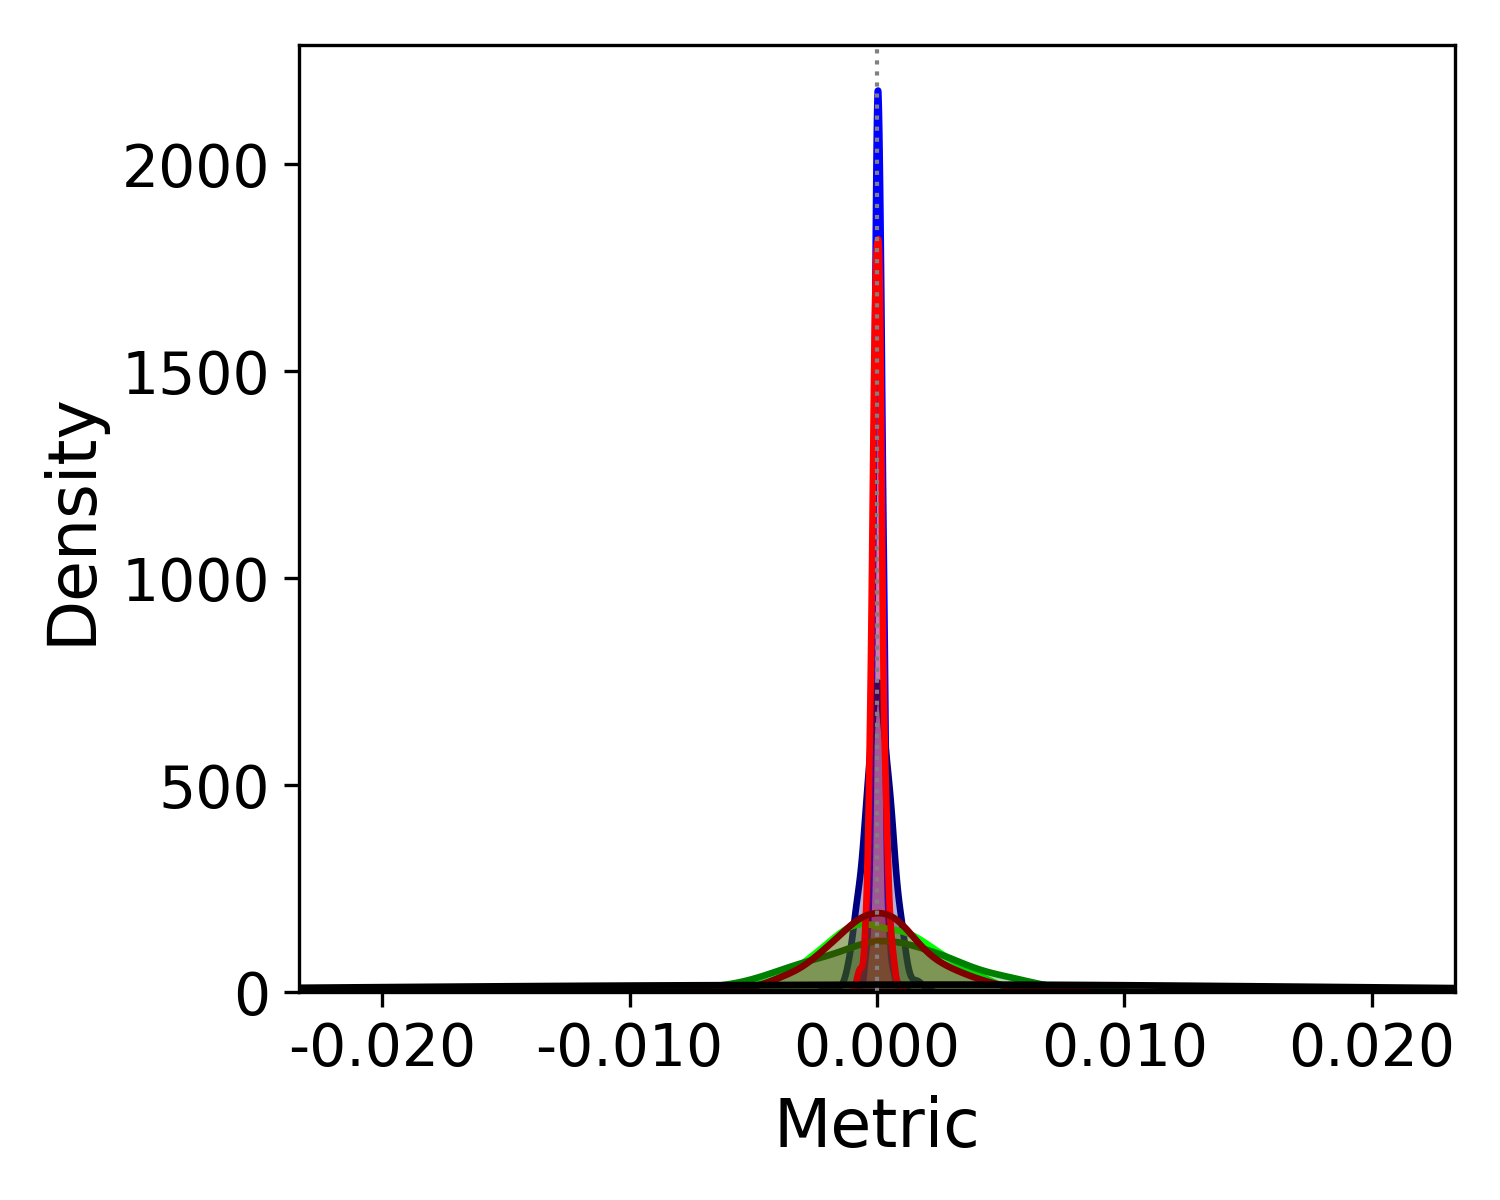
\includegraphics[width=\linewidth]{figs/SD_20_A_I_l1o.png}
        \caption{Adult: IID / LOO}
    \end{subfigure}
    \hfill
    \begin{subfigure}{0.24\textwidth}
        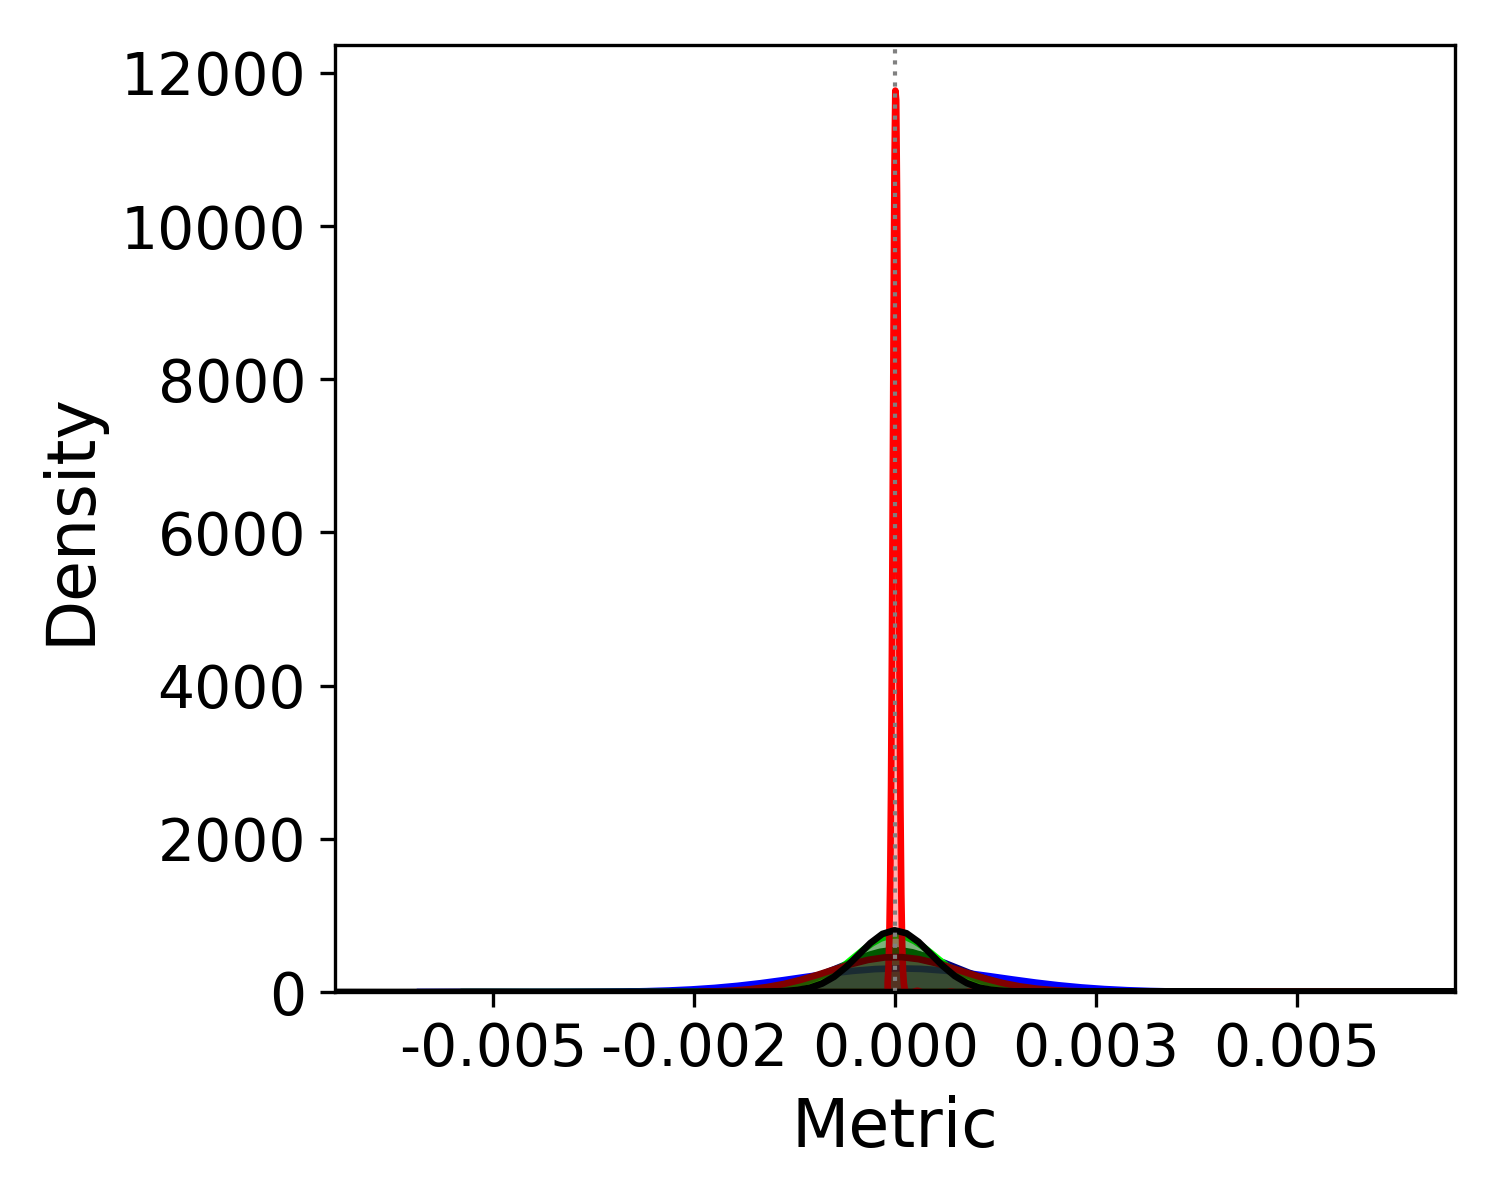
\includegraphics[width=\linewidth]{figs/SD_20_A_I_gtg.png}
        \caption{Adult: IID / GTG}
    \end{subfigure}
    \hfill
    \begin{subfigure}{0.24\textwidth}
        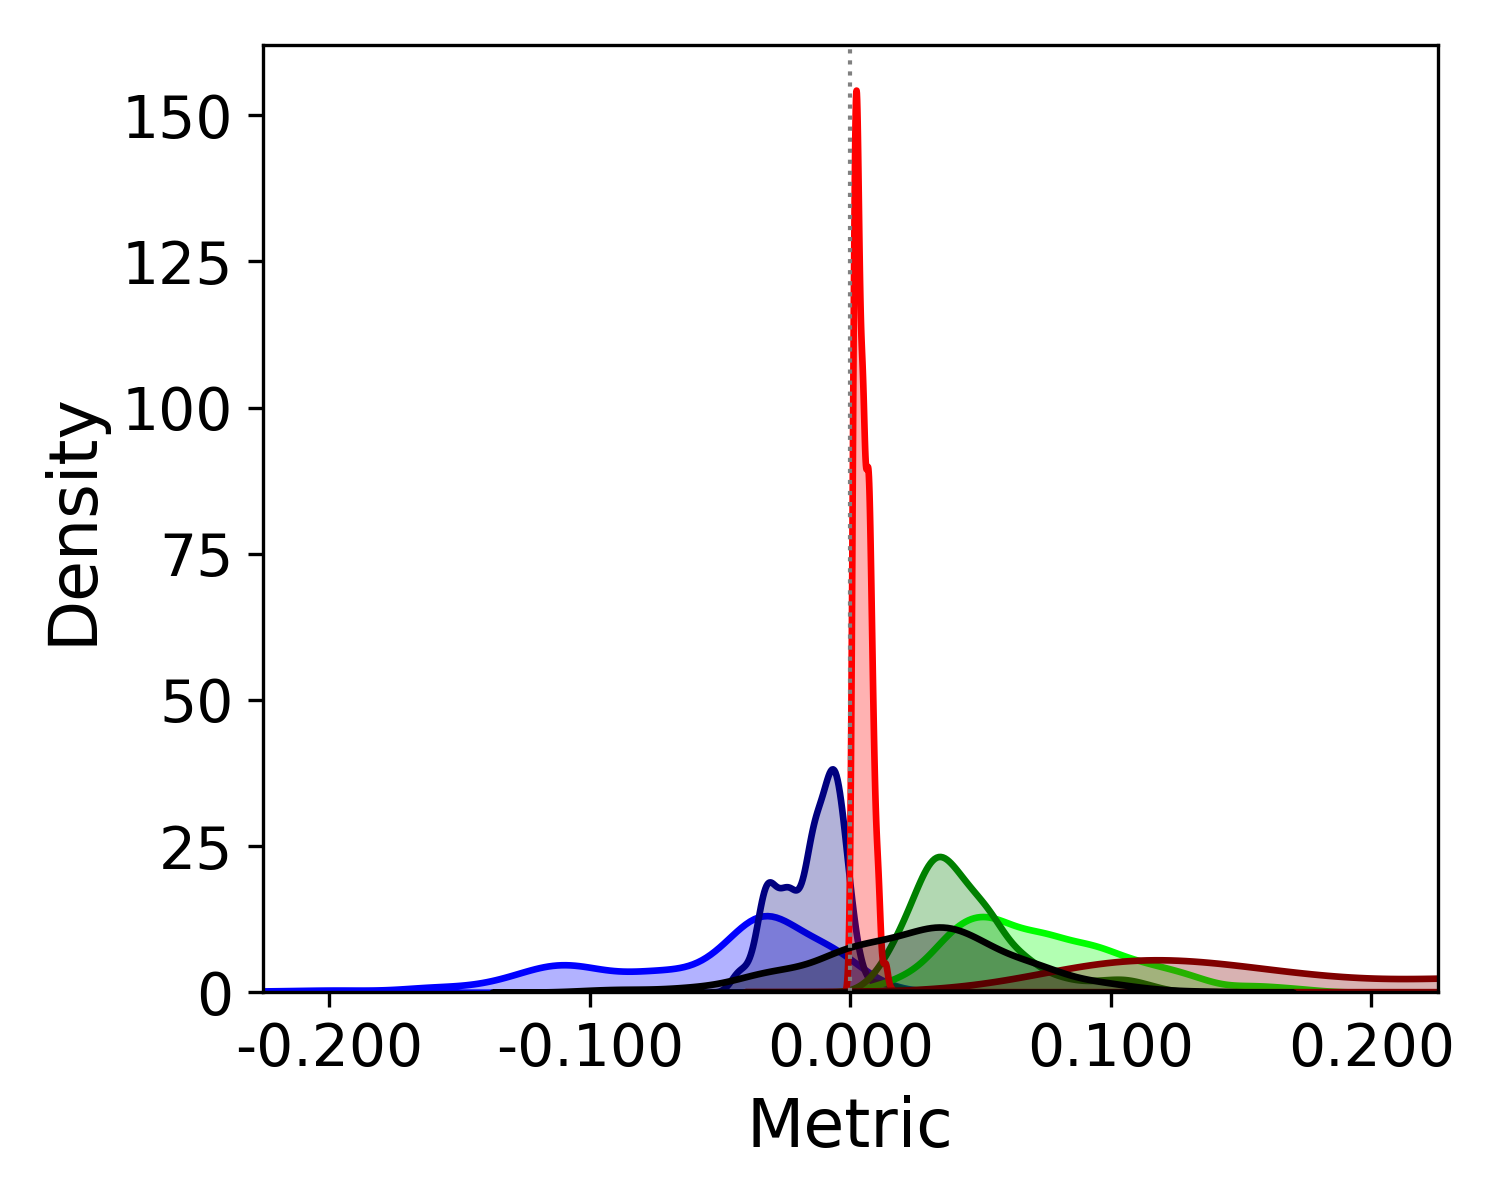
\includegraphics[width=\linewidth]{figs/SD_20_A_N_l1o.png}
        \caption{Adult: NIID / LOO}
    \end{subfigure}
    \hfill
    \begin{subfigure}{0.24\textwidth}
        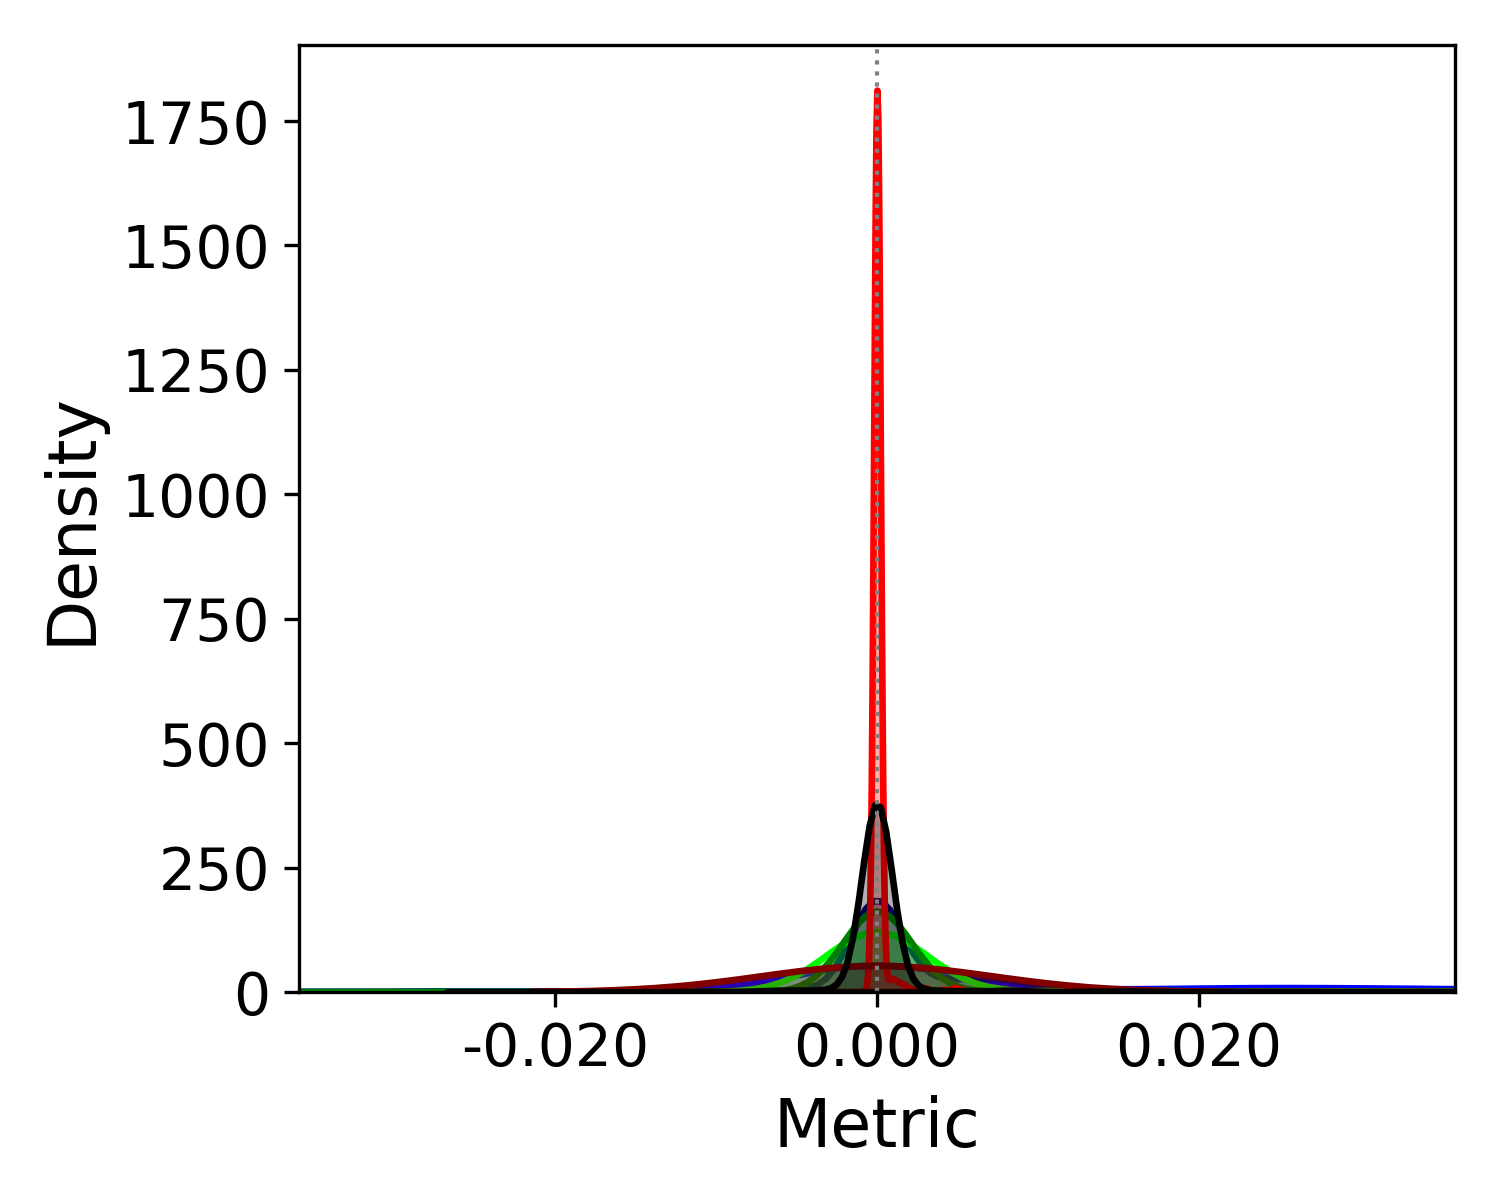
\includegraphics[width=\linewidth]{figs/SD_20_A_N_gtg.png}
        \caption{Adult: NIID / GTG}
    \end{subfigure}

    % CelebA - 20 Clients
    \begin{subfigure}{0.24\textwidth}
        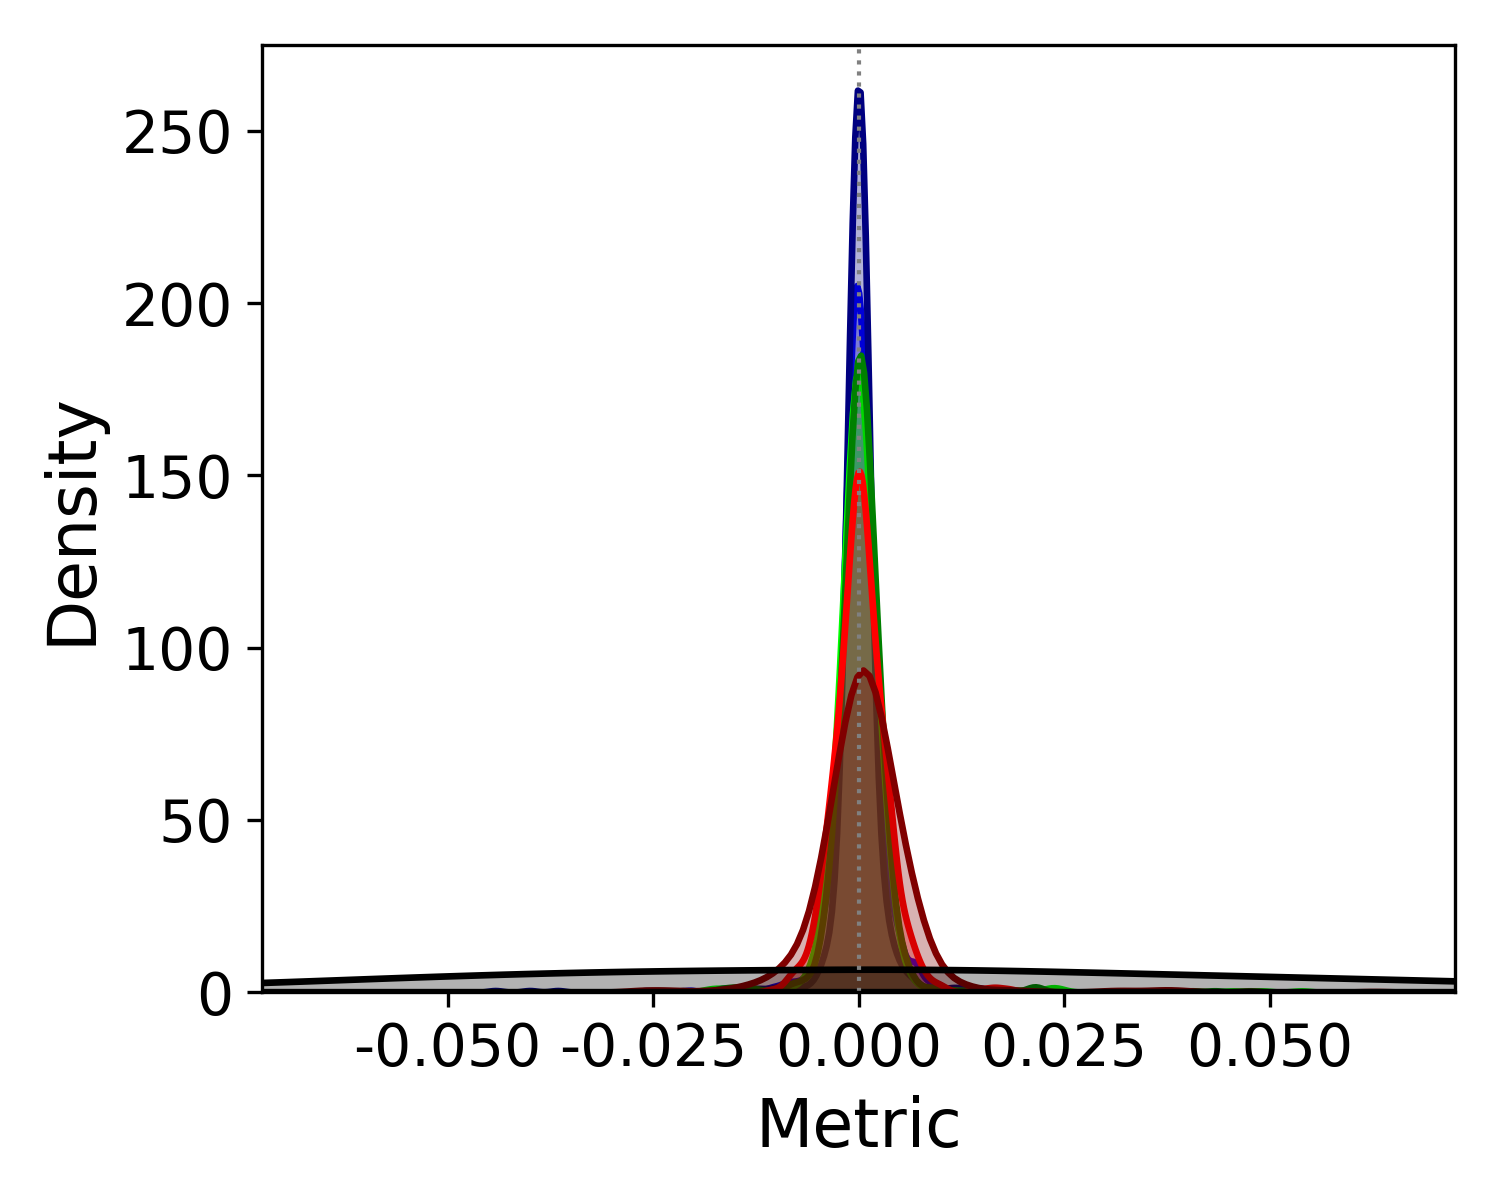
\includegraphics[width=\linewidth]{figs/SD_20_C_I_l1o.png}
        \caption{CelebA: IID / LOO}
    \end{subfigure}
    \hfill
    \begin{subfigure}{0.24\textwidth}
        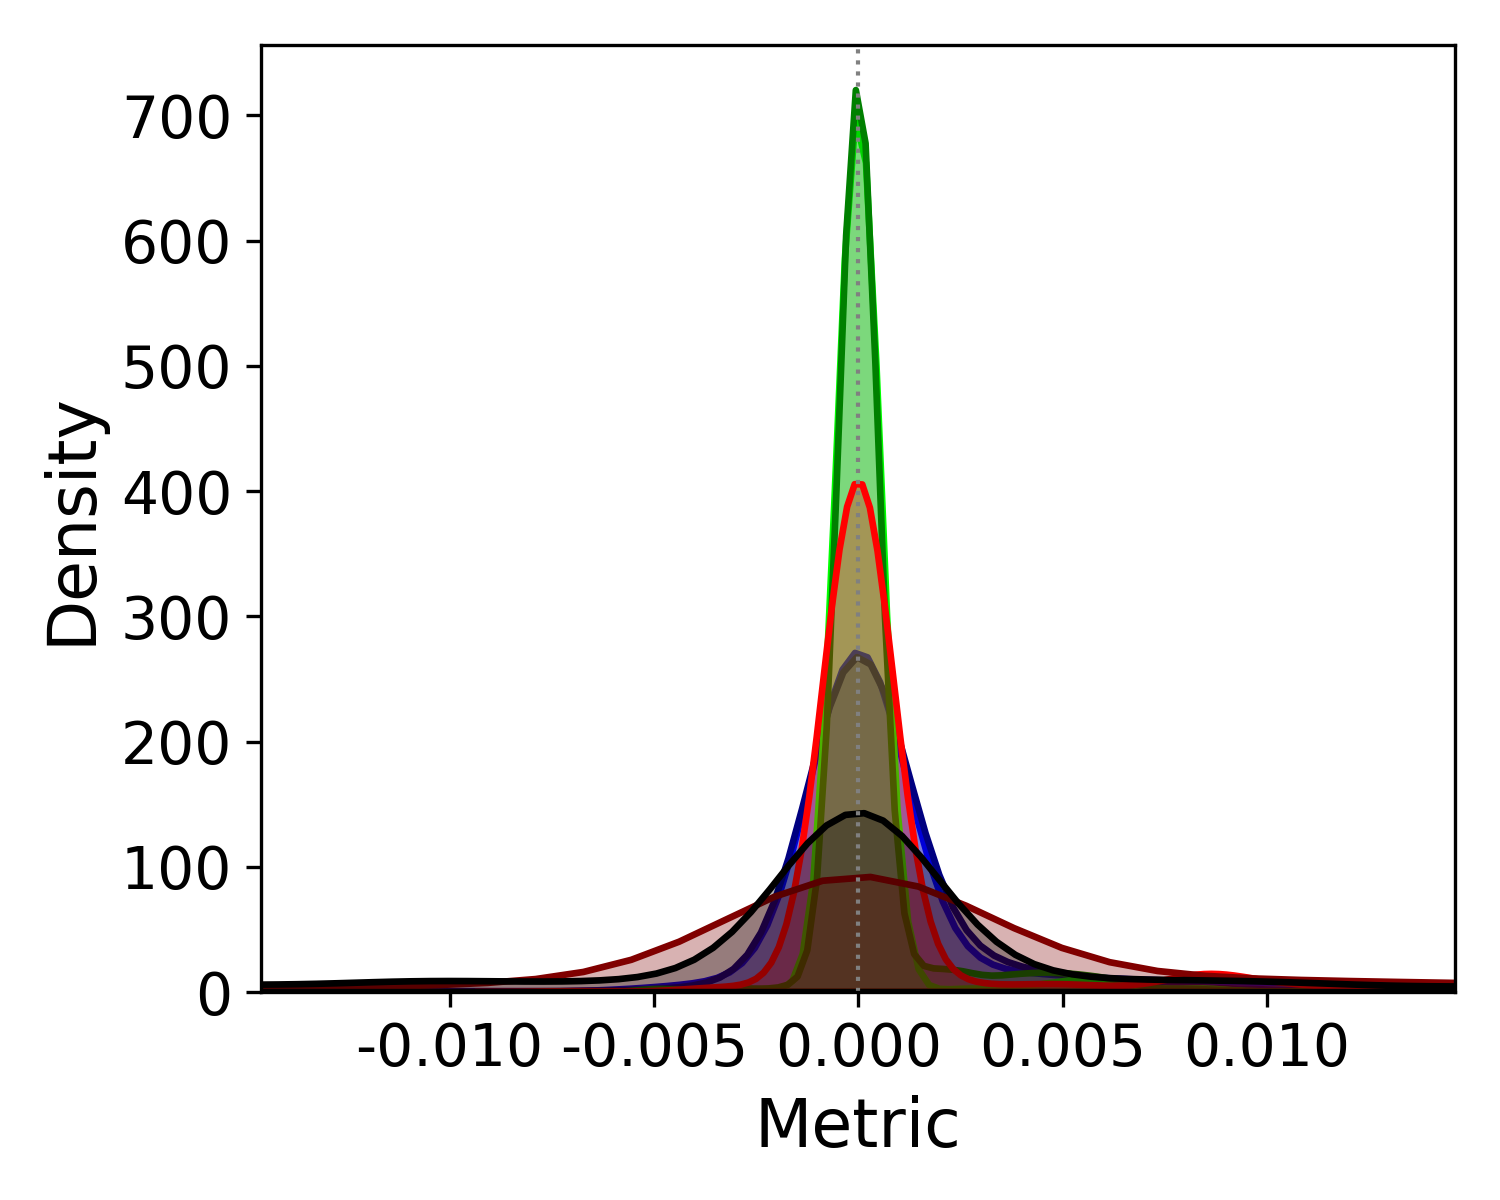
\includegraphics[width=\linewidth]{figs/SD_20_C_I_gtg.png}
        \caption{CelebA: IID / GTG}
    \end{subfigure}
    \hfill
    \begin{subfigure}{0.24\textwidth}
        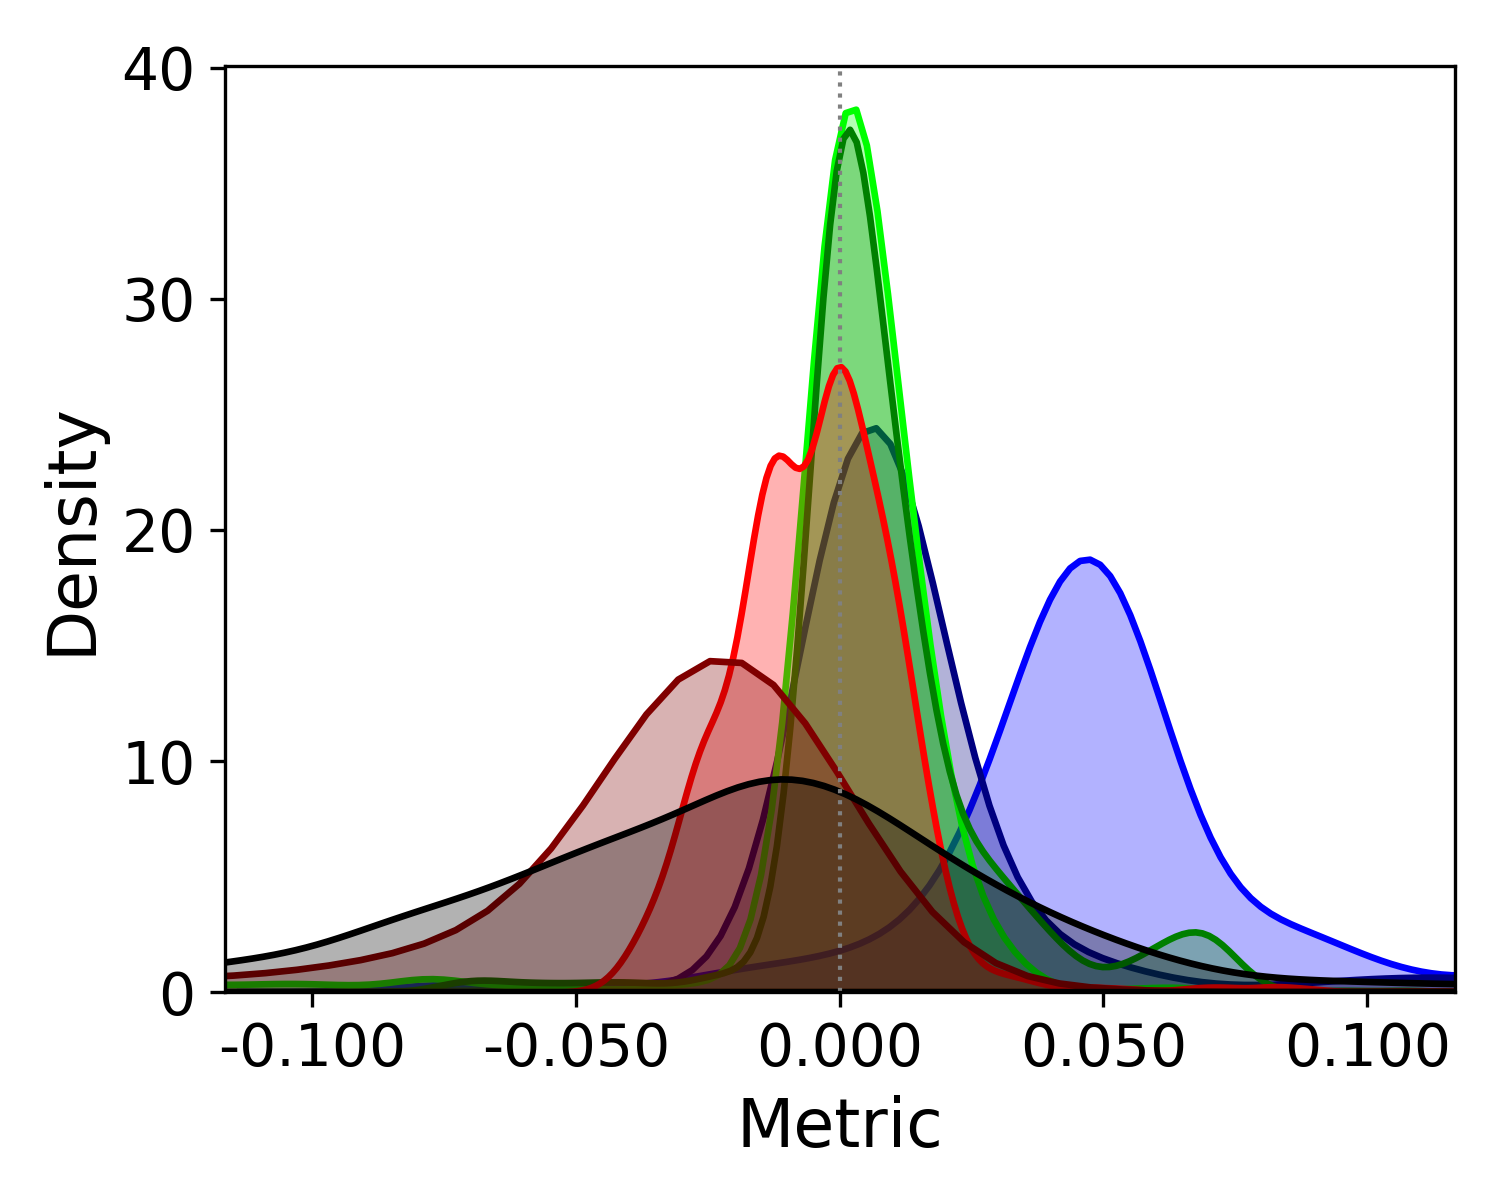
\includegraphics[width=\linewidth]{figs/SD_20_C_N_l1o.png}
        \caption{CelebA: NIID / LOO}
    \end{subfigure}
    \hfill
    \begin{subfigure}{0.24\textwidth}
        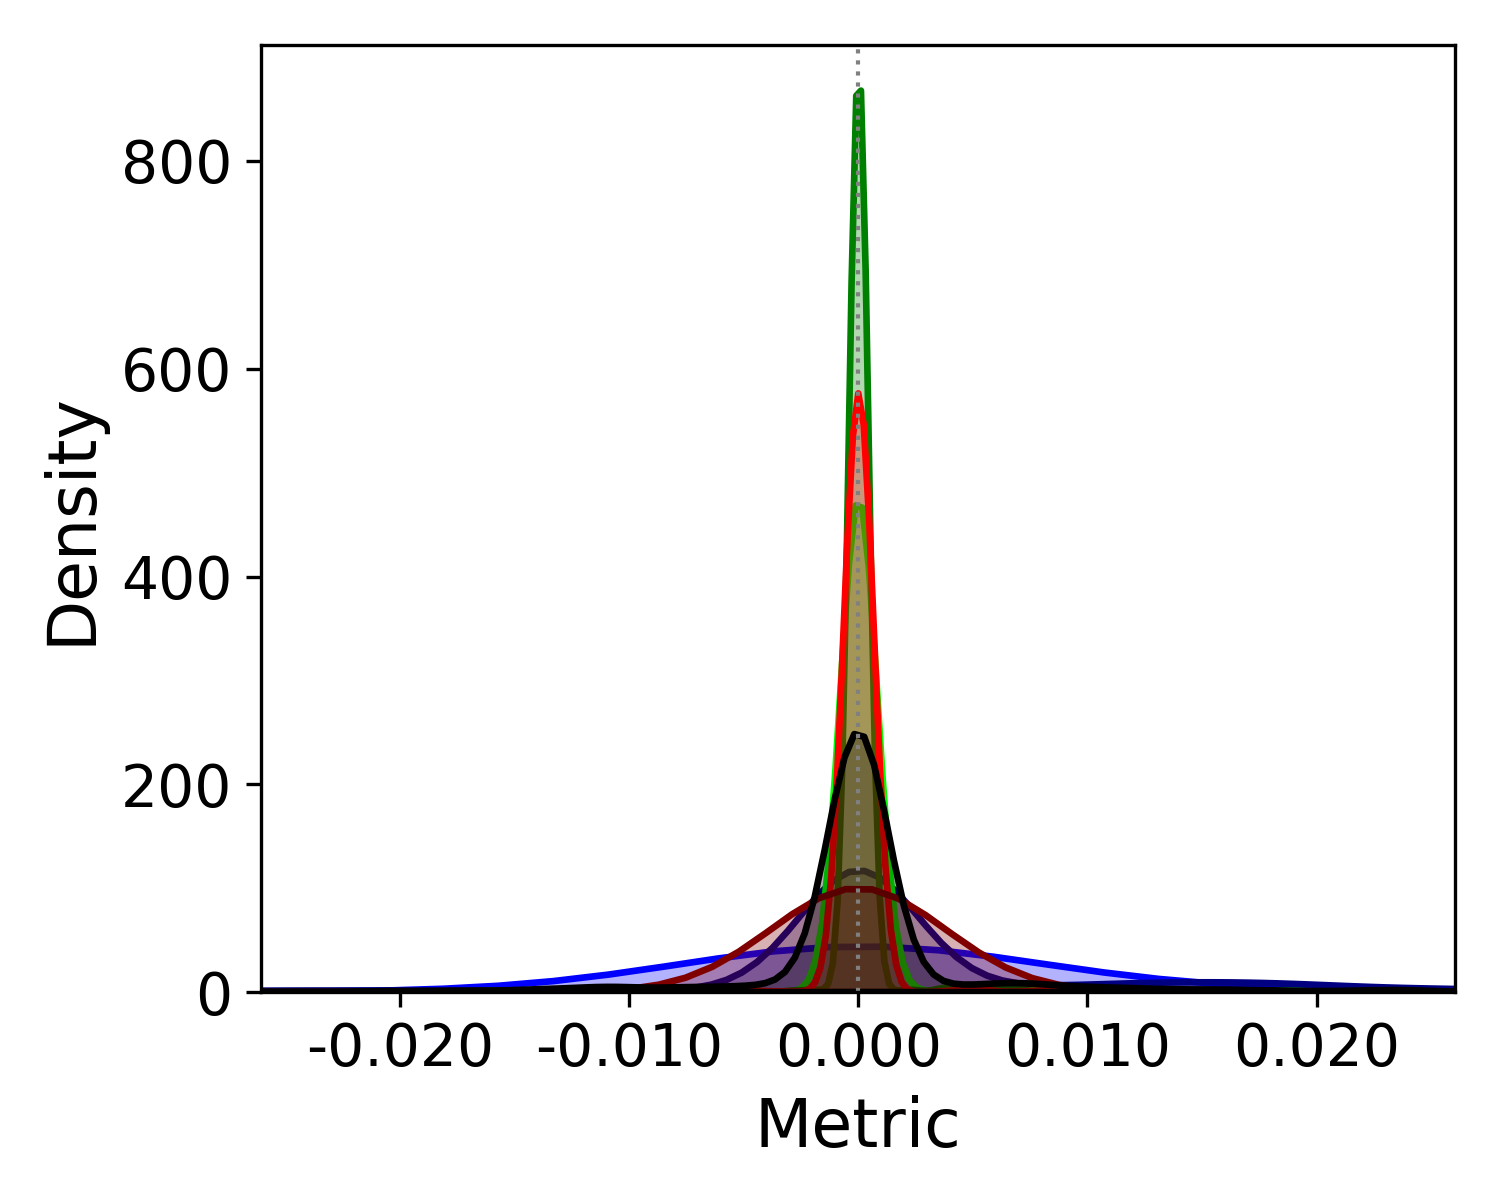
\includegraphics[width=\linewidth]{figs/SD_20_C_N_gtg.png}
        \caption{CelebA: NIID / GTG}
    \end{subfigure}

    % IMDB - 20 Clients
    \begin{subfigure}{0.24\textwidth}
        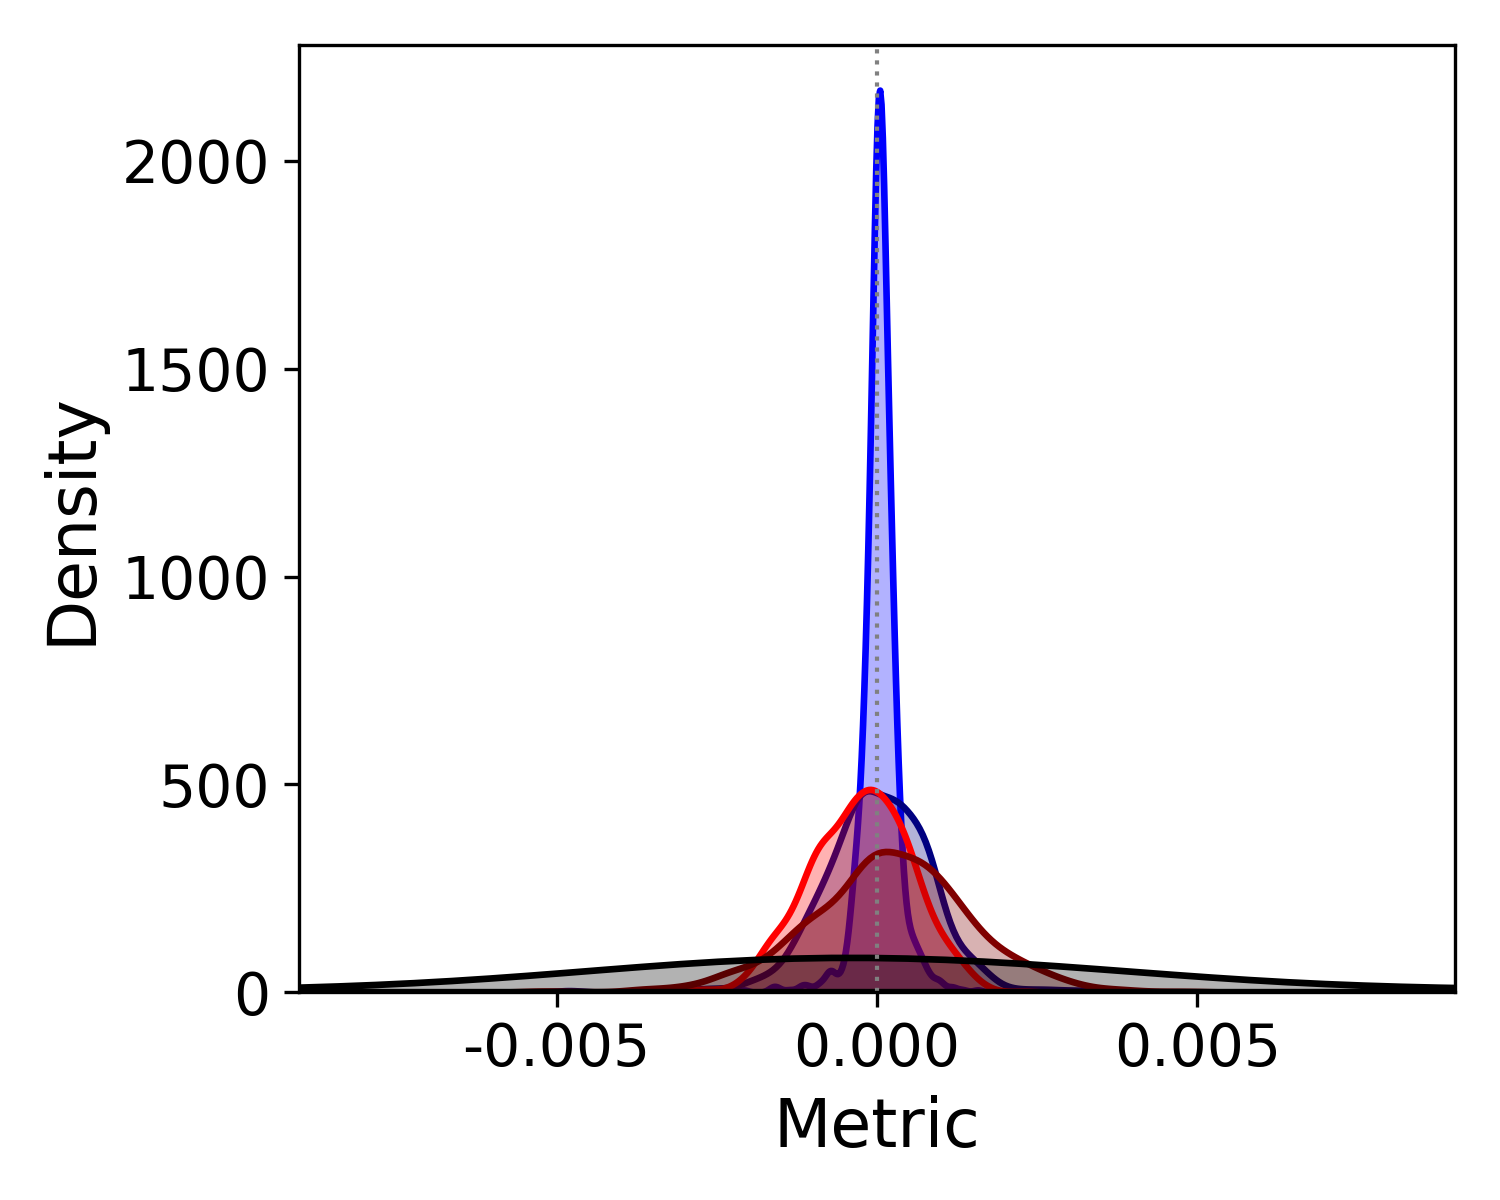
\includegraphics[width=\linewidth]{figs/SD_20_I_I_l1o.png}
        \caption{IMDB: IID / LOO}
    \end{subfigure}
    \hfill
    \begin{subfigure}{0.24\textwidth}
        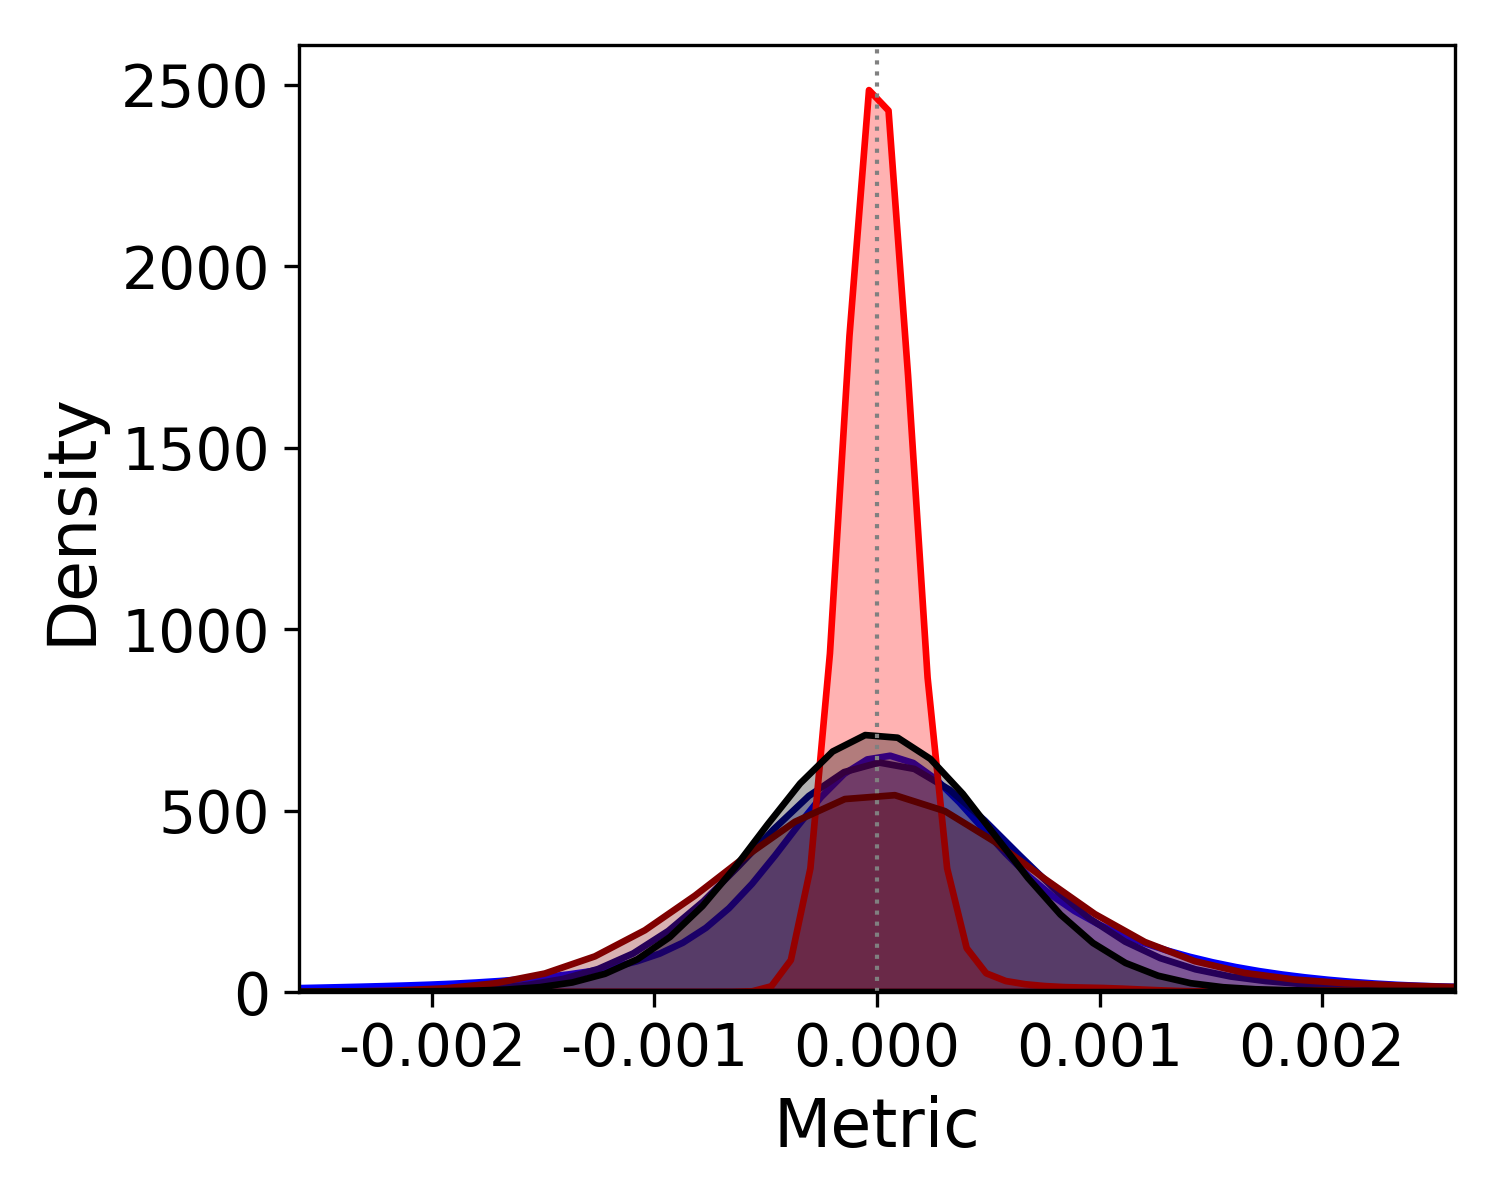
\includegraphics[width=\linewidth]{figs/SD_20_I_I_gtg.png}
        \caption{IMDB: IID / GTG}
    \end{subfigure}
    \hfill
    \begin{subfigure}{0.24\textwidth}
        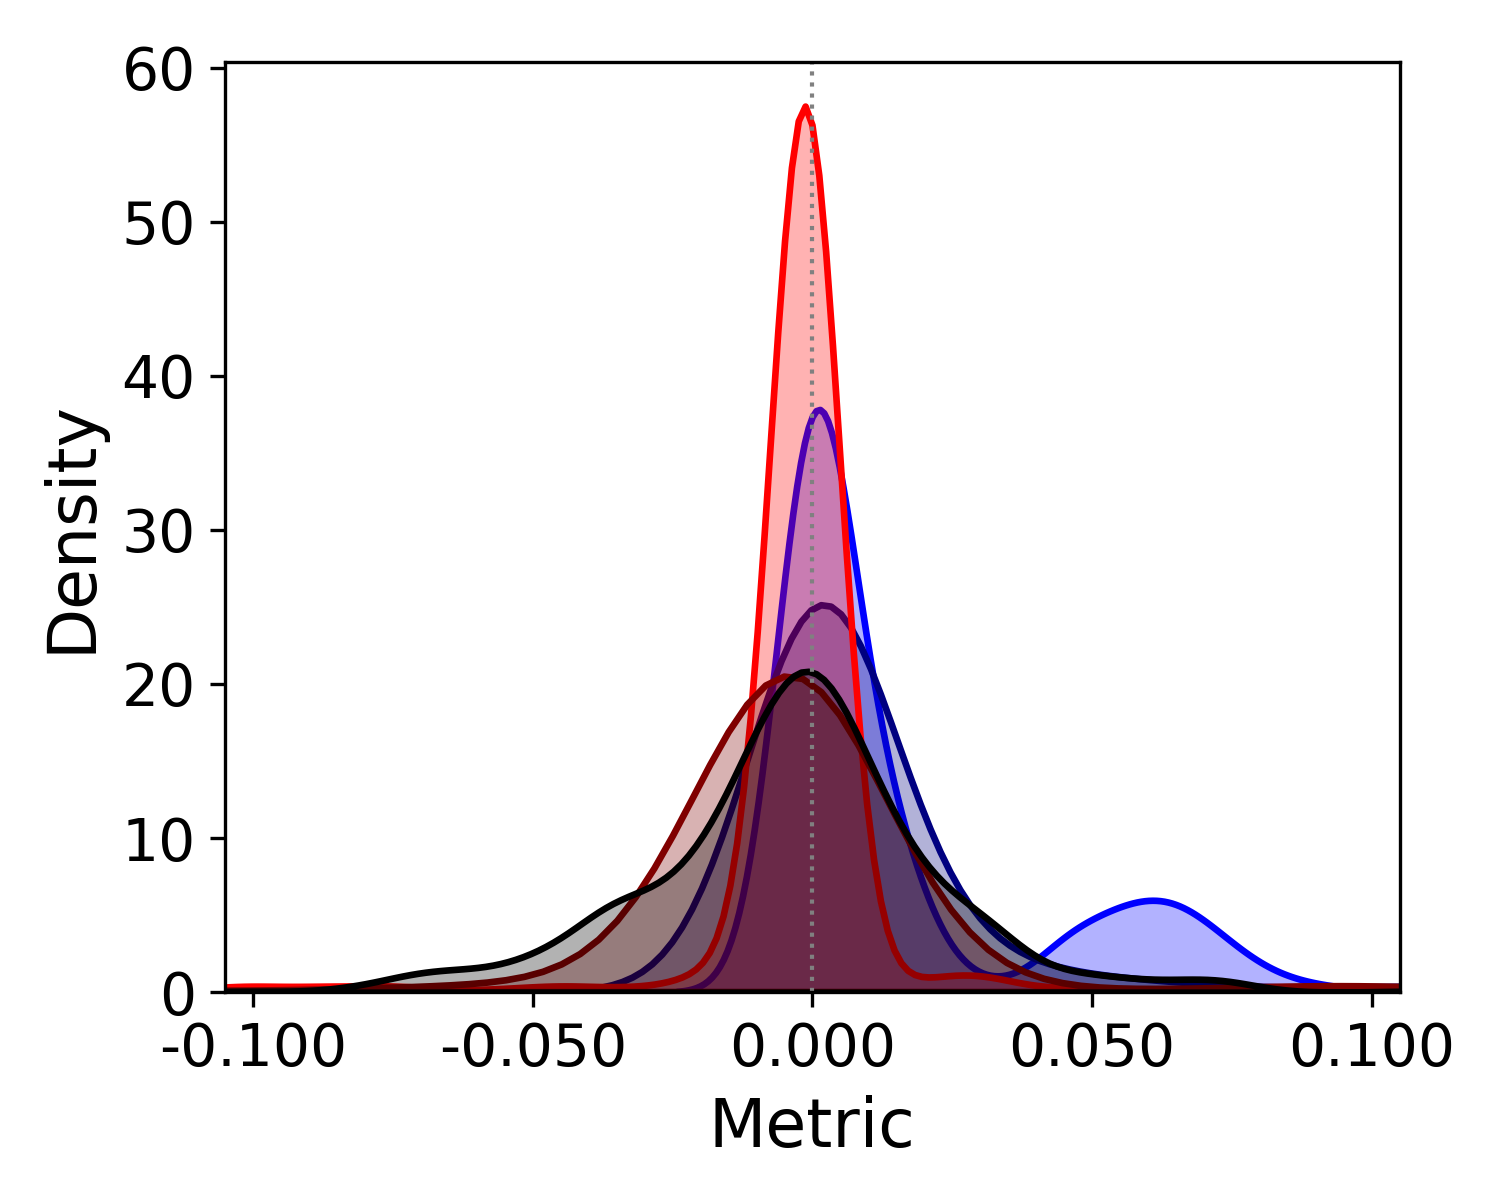
\includegraphics[width=\linewidth]{figs/SD_20_I_N_l1o.png}
        \caption{IMDB: NIID / LOO}
    \end{subfigure}
    \hfill
    \begin{subfigure}{0.24\textwidth}
        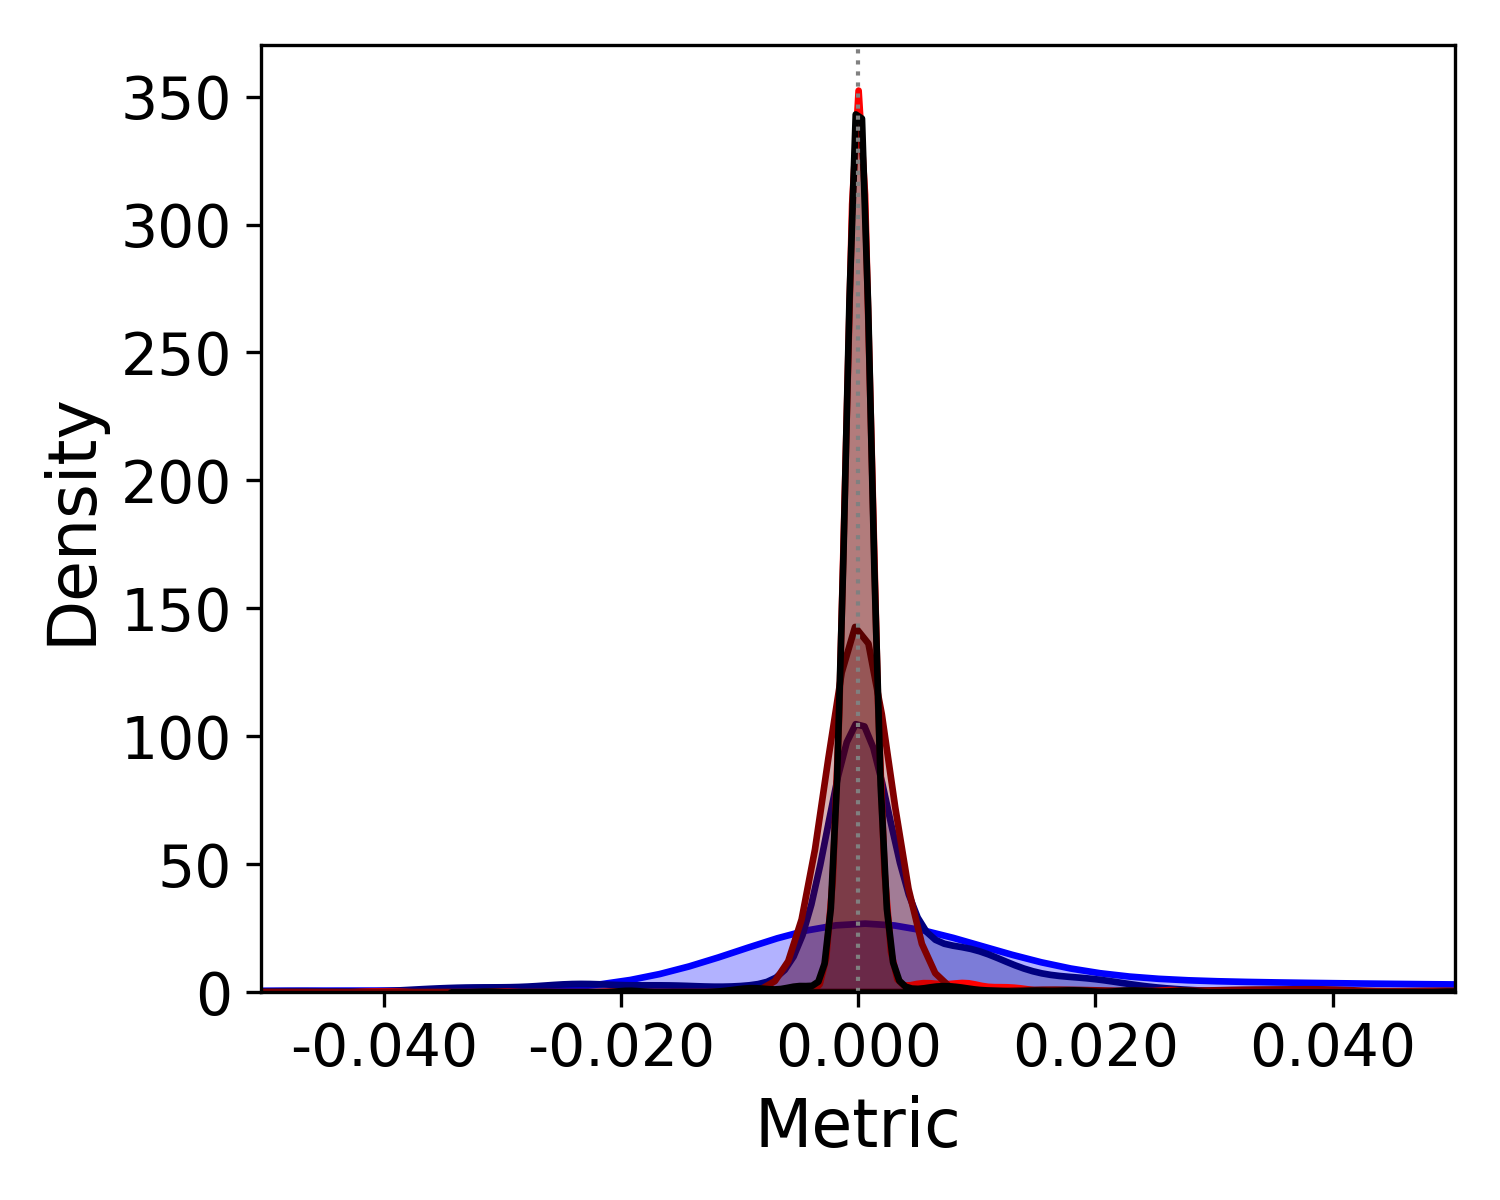
\includegraphics[width=\linewidth]{figs/SD_20_I_N_gtg.png}
        \caption{IMDB: NIID / GTG}
    \end{subfigure}
    
    \caption{Empirical score distributions (round $t=10$) for the 20-client scenario.}
    \label{fig:score_dist_20}
\end{figure}

Instead of examining clients in isolation, we now analyze the overarching distribution of their trustworthiness scores. Fig.~\ref{fig:score_dist_20} illustrate these distributions across all experimental configurations for $K=20$ ($K=4$ is in the Appendix). While both provide valuable insights, we focus our primary analysis on the 20-client scenario, as the higher client count yields more robust empirical density estimations. Under IID conditions, the score distributions uniformly collapse into sharp, narrow spikes centered precisely at zero. This perfectly aligns with federated learning theory: when data is homogeneously distributed, clients are statistically interchangeable. Consequently, the marginal contribution of any single client to the global model is effectively zero. 

However, when data becomes non-IID, these distributions flatten and widen significantly, revealing stark disparities in client value. Here, the choice of scoring mechanism plays a critical role. GTG-Shapley acts as a strong variance dampener; by averaging marginal contributions over many random permutations, it produces highly conservative, tightly bounded scores. In contrast, the LOO evaluation exposes extreme outliers, revealing distinct negative and positive distribution shifts. Crucially, because these distributions do not perfectly overlap, they expose stark, uncoupled trade-offs within the client pool. For instance, in the ADULT non-IID LOO setting, the performance and fairness distributions shift in opposite directions, which is a visual confirmation of their negative rank correlation. Finally, the concentration of these scores remains highly dataset-dependent. Reliability is tightly concentrated for ADULT, whereas resilience shows massive variance on CelebA. This confirms that different data modalities are inherently more sensitive to specific trustworthiness dimensions, fundamentally dictating how individual client contributions are valued across the federation.

\subsubsection*{Trustworthy Score Differences}

\begin{table}[!b]
    \centering
    \resizebox{\linewidth}{!}{
    \setlength{\tabcolsep}{2pt}
    \begin{tabular}{cccc||cc|cc|cc|cc|cc|cc}
        \multicolumn{4}{c||}{\multirow{2}{*}{\textbf{Setting}}}
        & \multicolumn{2}{c|}{\textbf{$\mathtt{acc}$}}
        & \multicolumn{2}{c|}{\textbf{$\mathtt{fairDP}$}}
        & \multicolumn{2}{c|}{\textbf{$\mathtt{fairEO}$}}
        & \multicolumn{2}{c|}{\textbf{$\mathtt{rel}$}}
        & \multicolumn{2}{c|}{\textbf{$\mathtt{res}$}}
        & \multicolumn{2}{c}{\textbf{$\mathtt{priv}$}} \\
        &&& & $\Phi$ & $L_2$ & $\Phi$ & $L_2$ & $\Phi$ & $L_2$ & $\Phi$ & $L_2$ & $\Phi$ & $L_2$ & $\Phi$ & $L_2$ \\
        \hline\hline
        \multirow{8}{*}{\rotatebox{90}{ADULT}} & \multirow{4}{*}{4} & \multirow{2}{*}{\rotatebox{90}{IID}} &
        LOO & $0.40 \pm 0.39$ & $0.00 \pm 0.00$ & $-0.20 \pm 0.69$ & $0.01 \pm 0.00$ & $0.40 \pm 0.49$ & $0.01 \pm 0.01$ & $0.40 \pm 0.36$ & $0.00 \pm 0.00$ & $-0.20 \pm 0.60$ & $0.00 \pm 0.00$ & $-0.60 \pm 0.53$ & $0.01 \pm 0.01$ \\
        &&& GTG & $-0.20 \pm 0.00$ & $0.00 \pm 0.00$ & $0.40 \pm 0.00$ & $0.01 \pm 0.00$ & $0.00 \pm 0.00$ & $0.01 \pm 0.01$ & \textemdash & $0.00 \pm 0.00$ & $-0.60 \pm 0.00$ & $0.00 \pm 0.00$ & $1.00 \pm 0.00$ & $0.00 \pm 0.00$ \\
        \cline{3-16}
        && \multirow{2}{*}{\rotatebox{90}{NIID}} &
        LOO & $1.00 \pm 0.08$ & $0.06 \pm 0.05$ & $0.00 \pm 0.79$ & $0.07 \pm 0.06$ & $0.60 \pm 0.78$ & $0.07 \pm 0.06$ & $-1.00 \pm 0.68$ & $0.10 \pm 0.06$ & $-1.00 \pm 0.66$ & $0.15 \pm 0.12$ & $-0.60 \pm 0.10$ & $0.12 \pm 0.05$ \\
        &&& GTG & $1.00 \pm 0.22$ & $0.11 \pm 0.12$ & $0.00 \pm 0.40$ & $0.10 \pm 0.11$ & $-0.80 \pm 0.59$ & $0.11 \pm 0.12$ & $-0.40 \pm 0.40$ & $0.11 \pm 0.12$ & $-0.80 \pm 0.31$ & $0.09 \pm 0.10$ & $-0.74 \pm 0.21$ & $0.11 \pm 0.11$ \\
        \cline{2-16}
        & \multirow{4}{*}{20} & \multirow{2}{*}{\rotatebox{90}{IID}} &
        LOO & $0.26 \pm 0.32$ & $0.00 \pm 0.00$ & $-0.16 \pm 0.58$ & $0.00 \pm 0.00$ & $0.01 \pm 0.36$ & $0.00 \pm 0.00$ & $-0.49 \pm 0.54$ & $0.00 \pm 0.00$ & $-0.26 \pm 0.47$ & $0.00 \pm 0.00$ & $-0.27 \pm 0.24$ & $0.01 \pm 0.01$ \\
        &&& GTG & \textemdash & $0.00 \pm 0.00$ & \textemdash & $0.00 \pm 0.00$ & \textemdash & $0.00 \pm 0.00$ & \textemdash & $0.00 \pm 0.00$ & \textemdash & $0.00 \pm 0.00$ & \textemdash & $0.00 \pm 0.00$ \\
        \cline{3-16}
        && \multirow{2}{*}{\rotatebox{90}{NIID}} &
        LOO & $0.94 \pm 0.47$ & $0.04 \pm 0.02$ & $-0.75 \pm 0.78$ & $0.12 \pm 0.05$ & $-0.76 \pm 0.61$ & $0.09 \pm 0.04$ & $-0.68 \pm 0.77$ & $0.05 \pm 0.03$ & $-0.70 \pm 0.78$ & $0.19 \pm 0.09$ & $-0.78 \pm 0.10$ & $0.09 \pm 0.04$ \\
        &&& GTG & $-0.03 \pm 0.21$ & $0.01 \pm 0.00$ & $-0.30 \pm 0.03$ & $0.01 \pm 0.00$ & $-0.53 \pm 0.06$ & $0.01 \pm 0.01$ & $-0.62 \pm 0.11$ & $0.01 \pm 0.00$ & $-0.53 \pm 0.11$ & $0.02 \pm 0.01$ & $-0.38 \pm 0.11$ & $0.01 \pm 0.00$ \\
        \hline
        \multirow{8}{*}{\rotatebox{90}{CelebA}} & \multirow{4}{*}{4} & \multirow{2}{*}{\rotatebox{90}{IID}} &
        LOO & $1.00 \pm 0.00$ & $0.00 \pm 0.00$ & $0.20 \pm 0.00$ & $0.01 \pm 0.00$ & $0.20 \pm 0.00$ & $0.01 \pm 0.00$ & $0.00 \pm 0.00$ & $0.03 \pm 0.00$ & $-0.20 \pm 0.00$ & $0.04 \pm 0.00$ & $0.80 \pm 0.00$ & $0.05 \pm 0.00$ \\
        &&& GTG & $-0.20 \pm 0.03$ & $0.00 \pm 0.01$ & $-0.40 \pm 0.29$ & $0.00 \pm 0.00$ & $-0.80 \pm 0.53$ & $0.00 \pm 0.00$ & $0.40 \pm 0.56$ & $0.01 \pm 0.01$ & $-0.20 \pm 0.59$ & $0.01 \pm 0.01$ & $0.60 \pm 0.55$ & $0.01 \pm 0.01$ \\
        \cline{3-16}
        && \multirow{2}{*}{\rotatebox{90}{NIID}} &
        LOO & $0.20 \pm 0.30$ & $0.01 \pm 0.00$ & $0.40 \pm 0.61$ & $0.03 \pm 0.01$ & $0.40 \pm 0.52$ & $0.03 \pm 0.01$ & $0.80 \pm 0.59$ & $0.02 \pm 0.01$ & $-0.80 \pm 0.54$ & $0.05 \pm 0.01$ & $0.40 \pm 0.26$ & $0.05 \pm 0.05$ \\
        &&& GTG & $1.00 \pm 0.02$ & $0.11 \pm 0.05$ & $-0.74 \pm 0.10$ & $0.13 \pm 0.06$ & $-0.20 \pm 0.34$ & $0.13 \pm 0.05$ & $0.77 \pm 0.61$ & $0.13 \pm 0.05$ & $-0.77 \pm 0.09$ & $0.19 \pm 0.06$ & $-0.74 \pm 0.51$ & $0.13 \pm 0.06$ \\
        \cline{2-16}
        & \multirow{4}{*}{20} & \multirow{2}{*}{\rotatebox{90}{IID}} &
        LOO & $0.54 \pm 0.14$ & $0.00 \pm 0.00$ & $-0.12 \pm 0.30$ & $0.00 \pm 0.00$ & $-0.15 \pm 0.28$ & $0.00 \pm 0.00$ & $0.23 \pm 0.15$ & $0.00 \pm 0.00$ & $0.40 \pm 0.17$ & $0.00 \pm 0.00$ & $-0.30 \pm 0.12$ & $0.02 \pm 0.03$ \\
        &&& GTG & $0.50 \pm 0.22$ & $0.00 \pm 0.00$ & $0.22 \pm 0.14$ & $0.00 \pm 0.00$ & $0.01 \pm 0.12$ & $0.00 \pm 0.00$ & $0.06 \pm 0.00$ & $0.00 \pm 0.00$ & $0.28 \pm 0.07$ & $0.00 \pm 0.00$ & $0.20 \pm 0.06$ & $0.00 \pm 0.00$ \\
        \cline{3-16}
        && \multirow{2}{*}{\rotatebox{90}{NIID}} &
        LOO & $0.60 \pm 0.35$ & $0.04 \pm 0.00$ & $0.27 \pm 0.17$ & $0.04 \pm 0.01$ & $0.35 \pm 0.25$ & $0.04 \pm 0.01$ & $-0.31 \pm 0.35$ & $0.04 \pm 0.02$ & $-0.41 \pm 0.27$ & $0.06 \pm 0.01$ & $0.04 \pm 0.13$ & $0.03 \pm 0.01$ \\
        &&& GTG & $0.53 \pm 0.18$ & $0.02 \pm 0.01$ & $-0.42 \pm 0.37$ & $0.02 \pm 0.01$ & $0.14 \pm 0.39$ & $0.02 \pm 0.01$ & $-0.43 \pm 0.39$ & $0.02 \pm 0.01$ & $-0.43 \pm 0.37$ & $0.03 \pm 0.01$ & $-0.51 \pm 0.20$ & $0.02 \pm 0.01$ \\
        \hline
        \multirow{8}{*}{\rotatebox{90}{IMDB}} & \multirow{4}{*}{4} & \multirow{2}{*}{\rotatebox{90}{IID}} &
        LOO & $0.60 \pm 0.45$ & $0.00 \pm 0.00$ & \textemdash & \textemdash & \textemdash & \textemdash & $-0.40 \pm 0.61$ & $0.00 \pm 0.00$ & $0.40 \pm 0.53$ & $0.00 \pm 0.00$ & $-0.80 \pm 0.54$ & $0.01 \pm 0.01$ \\
        &&& GTG & $0.80 \pm 0.44$ & $0.00 \pm 0.00$ & \textemdash & \textemdash & \textemdash & \textemdash & $-0.80 \pm 0.50$ & $0.00 \pm 0.00$ & $-0.40 \pm 0.69$ & $0.00 \pm 0.00$ & $-1.00 \pm 0.42$ & $0.01 \pm 0.01$ \\
        \cline{3-16}
        && \multirow{2}{*}{\rotatebox{90}{NIID}} &
        LOO & $1.00 \pm 0.00$ & $0.03 \pm 0.01$ & \textemdash & \textemdash & \textemdash & \textemdash & $-0.80 \pm 0.29$ & $0.07 \pm 0.01$ & $-1.00 \pm 0.10$ & $0.10 \pm 0.02$ & $-0.80 \pm 0.20$ & $0.08 \pm 0.02$ \\
        &&& GTG & $0.95 \pm 0.09$ & $0.07 \pm 0.03$ & \textemdash & \textemdash & \textemdash & \textemdash & $-0.54 \pm 0.10$ & $0.10 \pm 0.03$ & $-0.54 \pm 0.10$ & $0.11 \pm 0.03$ & $0.11 \pm 0.44$ & $0.09 \pm 0.03$ \\
        \cline{2-16}
        & \multirow{4}{*}{20} & \multirow{2}{*}{\rotatebox{90}{IID}} &
        LOO & $0.43 \pm 0.18$ & $0.00 \pm 0.00$ & \textemdash & \textemdash & \textemdash & \textemdash & $0.07 \pm 0.12$ & $0.00 \pm 0.00$ & $-0.44 \pm 0.25$ & $0.00 \pm 0.00$ & $0.04 \pm 0.23$ & $0.00 \pm 0.00$ \\
        &&& GTG & $0.42 \pm 0.05$ & $0.00 \pm 0.00$ & \textemdash & \textemdash & \textemdash & \textemdash & $0.02 \pm 0.10$ & $0.00 \pm 0.00$ & $-0.36 \pm 0.21$ & $0.00 \pm 0.00$ & $0.35 \pm 0.23$ & $0.00 \pm 0.00$ \\
        \cline{3-16}
        && \multirow{2}{*}{\rotatebox{90}{NIID}} &
        LOO & $0.77 \pm 0.13$ & $0.00 \pm 0.00$ & \textemdash & \textemdash & \textemdash & \textemdash & $-0.79 \pm 0.16$ & $0.00 \pm 0.00$ & $-0.83 \pm 0.23$ & $0.01 \pm 0.00$ & $0.11 \pm 0.20$ & $0.01 \pm 0.01$ \\
        &&& GTG & $0.84 \pm 0.17$ & $0.04 \pm 0.01$ & \textemdash & \textemdash & \textemdash & \textemdash & $-0.57 \pm 0.12$ & $0.05 \pm 0.02$ & $-0.57 \pm 0.22$ & $0.05 \pm 0.02$ & $0.26 \pm 0.29$ & $0.05 \pm 0.02$ \\
    \end{tabular}}
    \caption{Comparing both the $\mathtt{LOO}$ and $\mathtt{GTG}$-based performance scores ($\mathtt{loss}$) to the other trustworthy metrics. Here, I and N stand for IID and non-IID data distributions, respectively. The primary correlation scores ($\Phi$) and distances ($L_2$) are calculated on seed-averaged contributions (matching visual heatmaps), while the standard deviations ($\pm$) represent the variance across individual seed-level score calculations. $\Phi$ is shown as \textemdash{} where the contribution scores are degenerate (equal), leaving the rank correlation undefined.}
    \label{tab:score_diff_merged}
\end{table}



We also study the discrepancy between the multi-dimensional trustworthiness scores and the baseline performance score. Because the standard federated training process explicitly optimizes to minimize the loss function ($\mathtt{loss}$), we utilize the client's contribution to this loss reduction as the baseline representation of standard performance. To quantify the deviation from this baseline, we use both a relative and an absolute metric. We apply the Spearman correlation coefficient ($\Phi$)~\cite{wissler1905spearman} to capture discrepancies in the client orderings (i.e., rankings) implied by the scores. This value falls in the range $[-1, 1]$, where positive/negative values imply a positive/negative correlation, and values near zero indicate statistical independence. While such rank correlations are crucial for relative contribution evaluation, they do not capture the full magnitude of the discrepancies: an ordered list of contributions $[1, 2, 3]$ is identical rank-wise to $[1, 2, 100]$. Thus, we also employ the $L_2$ difference (RMSE) to capture the absolute numerical distance between a client's various scores. This absolute measurement becomes exceptionally important if the system allocates monetary gains or rewards based on these contributions. Both values are reported in Tab.~\ref{tab:score_diff_merged}, which exhaustively compares the $\mathtt{LOO}$ and $\mathtt{GTG}$ evaluation methods across all settings.

\begin{figure}[!b]
    \centering
    
    % ADULT - IID
    \begin{subfigure}{0.24\textwidth}
        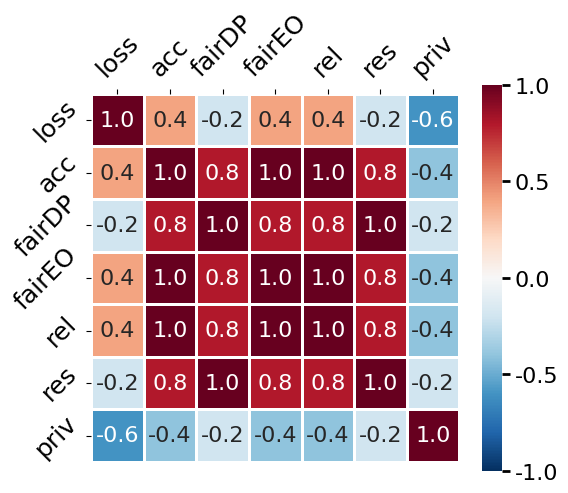
\includegraphics[width=\linewidth]{figs/H_4_A_I_l1o.png}
        \caption{Adult: 4 I / LOO}
    \end{subfigure}
    \hfill
    \begin{subfigure}{0.24\textwidth}
        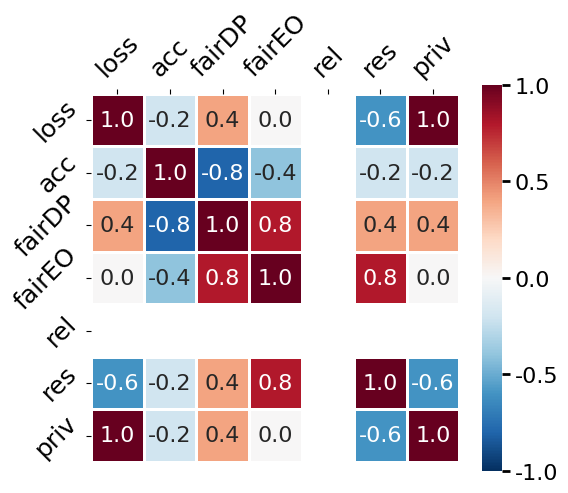
\includegraphics[width=\linewidth]{figs/H_4_A_I_gtg.png}
        \caption{Adult: 4 I / GTG}
    \end{subfigure}
    \hfill
    \begin{subfigure}{0.24\textwidth}
        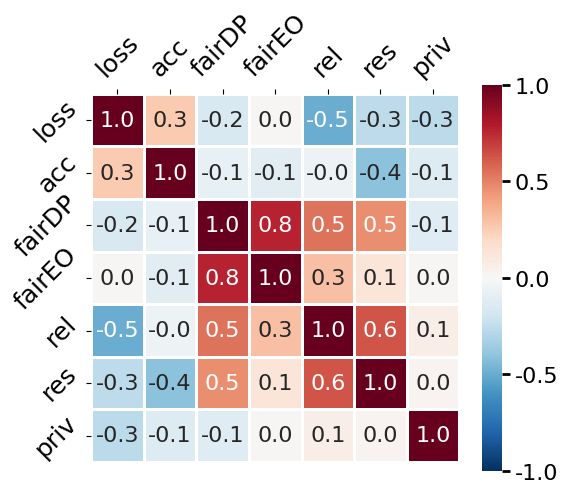
\includegraphics[width=\linewidth]{figs/H_20_A_I_l1o.png}
        \caption{Adult: 20 I / LOO}
    \end{subfigure}
    \hfill
    \begin{subfigure}{0.24\textwidth}
        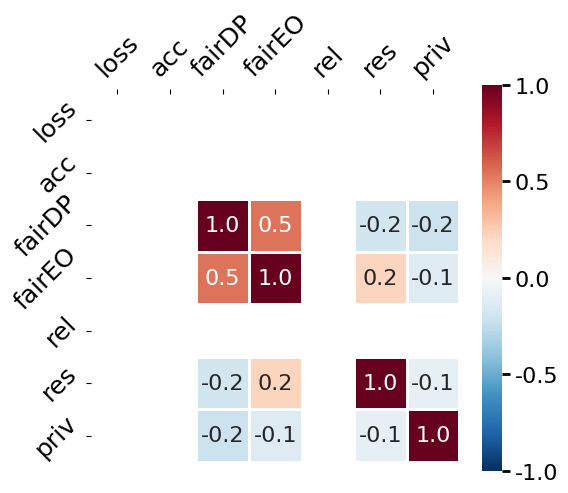
\includegraphics[width=\linewidth]{figs/H_20_A_I_gtg.png}
        \caption{Adult: 20 I / GTG}
    \end{subfigure}

    % CelebA - IID
    \begin{subfigure}{0.24\textwidth}
        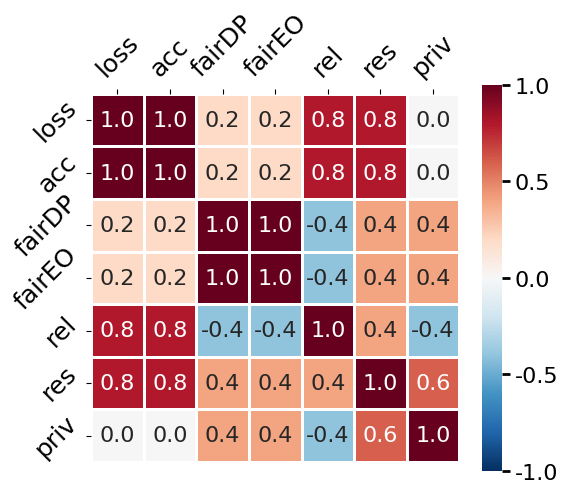
\includegraphics[width=\linewidth]{figs/H_4_C_I_l1o.png}
        \caption{CelebA: 4 I / LOO}
    \end{subfigure}
    \hfill
    \begin{subfigure}{0.24\textwidth}
        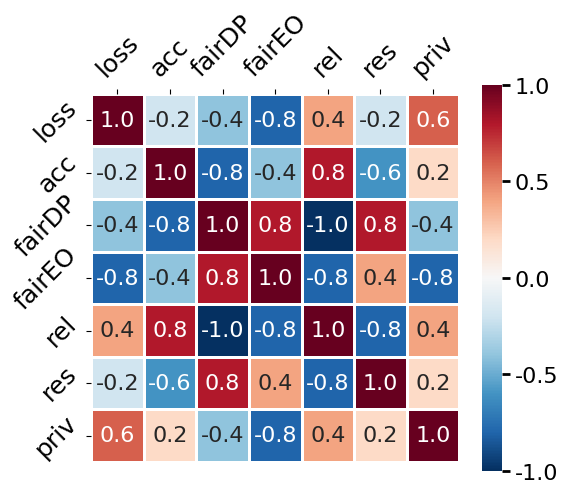
\includegraphics[width=\linewidth]{figs/H_4_C_I_gtg.png}
        \caption{CelebA: 4 I / GTG}
    \end{subfigure}
    \hfill
    \begin{subfigure}{0.24\textwidth}
        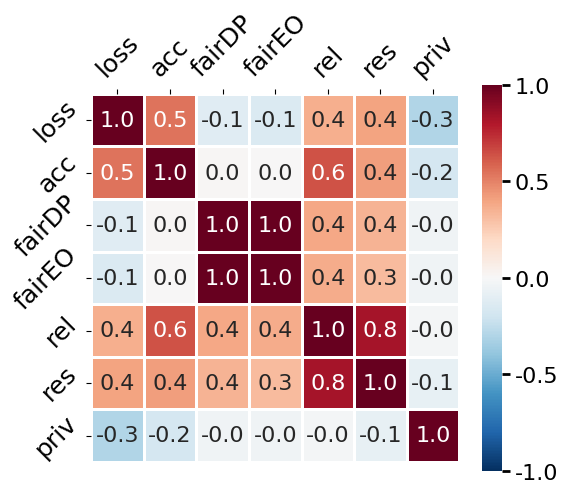
\includegraphics[width=\linewidth]{figs/H_20_C_I_l1o.png}
        \caption{CelebA: 20 I / LOO}
    \end{subfigure}
    \hfill
    \begin{subfigure}{0.24\textwidth}
        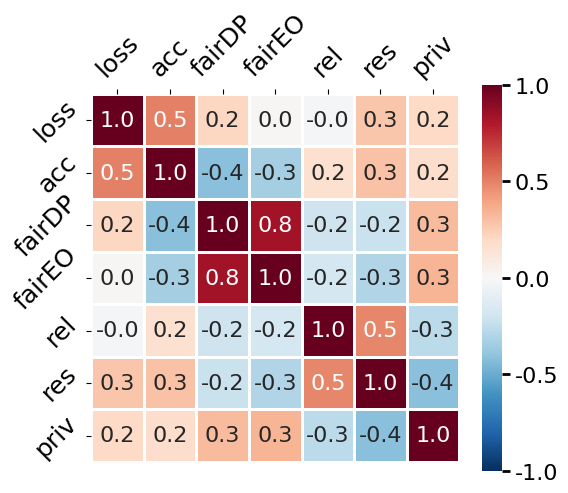
\includegraphics[width=\linewidth]{figs/H_20_C_I_gtg.png}
        \caption{CelebA: 20 I / GTG}
    \end{subfigure}

    % IMDB - IID
    \begin{subfigure}{0.24\textwidth}
        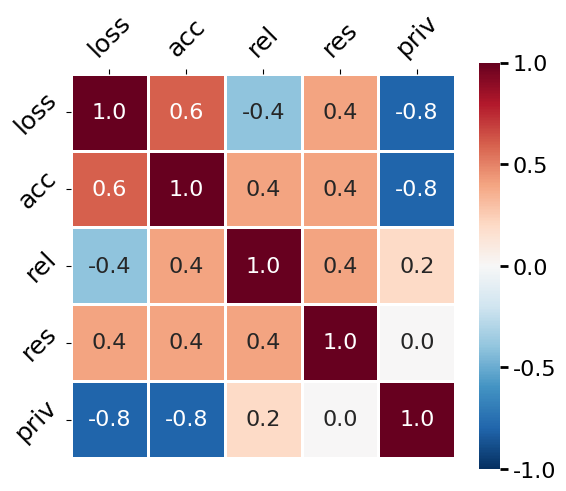
\includegraphics[width=\linewidth]{figs/H_4_I_I_l1o.png}
        \caption{IMDB: 4 I / LOO}
    \end{subfigure}
    \hfill
    \begin{subfigure}{0.24\textwidth}
        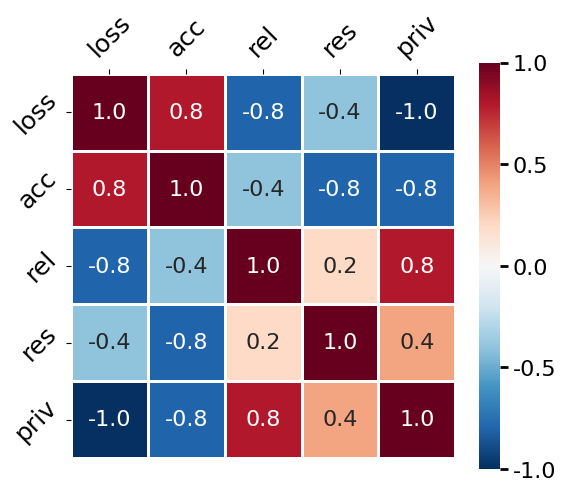
\includegraphics[width=\linewidth]{figs/H_4_I_I_gtg.png}
        \caption{IMDB: 4 I / GTG}
    \end{subfigure}
    \hfill
    \begin{subfigure}{0.24\textwidth}
        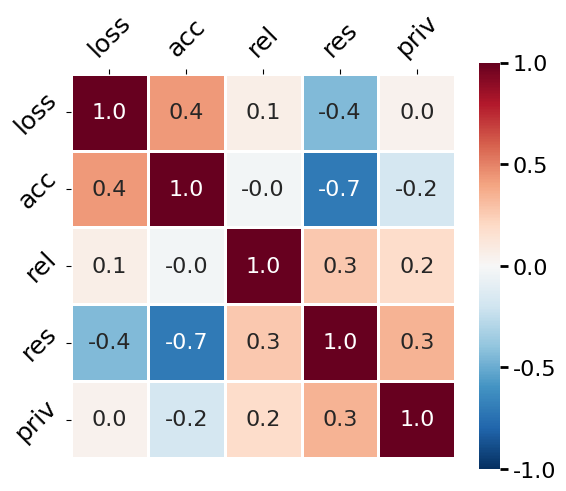
\includegraphics[width=\linewidth]{figs/H_20_I_I_l1o.png}
        \caption{IMDB: 20 I / LOO}
    \end{subfigure}
    \hfill
    \begin{subfigure}{0.24\textwidth}
        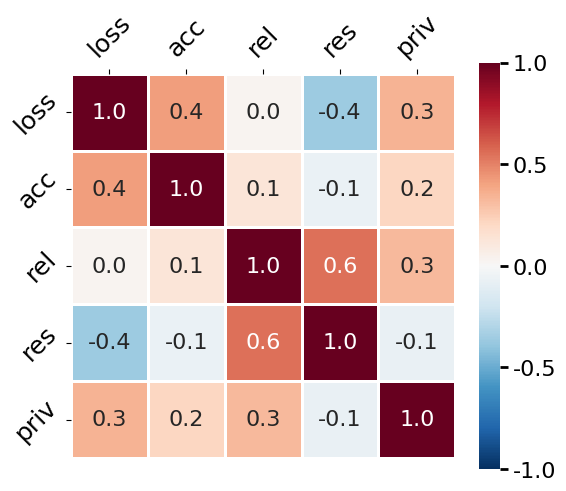
\includegraphics[width=\linewidth]{figs/H_20_I_I_gtg.png}
        \caption{IMDB: 20 I / GTG}
    \end{subfigure}
    
    \caption{Heatmap of the pair-wise score correlations (round $t=10$) for all IID scenarios. Degenerate (equal) scores yield undefined correlations and are left blank.}
    \label{fig:score_heat_IID}
\end{figure}

\subsubsection*{Trustworthy Score Correlations}

Lastly, instead of comparing the trustworthiness scores solely to the performance baseline, we evaluate their relationships against each other. This pairwise correlation analysis is visualized as heatmaps using Spearman's rank correlation coefficient in Fig.~\ref{fig:score_heat_IID} for the IID scenarios and Fig.~\ref{fig:score_heat_NIID} for the non-IID scenarios. When comparing data distributions, the IID settings (especially with a small client pool of $K=4$) often exhibit artificially broad, high correlations across the board. Because clients hold statistically identical data shards in an IID setup, their marginal contributions scale uniformly regardless of the metric. However, the realistic non-IID scenarios reveal the true, complex dynamics of the federation. These heatmaps confirm that performance-based evaluations are poor proxies for a client's overarching trustworthiness. Across the datasets in non-IID settings, correlations between the performance metrics and the trustworthiness metrics are frequently low or explicitly negative. This highlights strict operational trade-offs where optimizing exclusively for utility can actively degrade trust.

Conversely, clear blocks of high positive correlation emerge among metrics from the same conceptual family: the two fairness scores form a strongly correlated cluster across the ADULT and CelebA datasets, and on ADULT and IMDB the two robustness scores track each other, reflecting their shared focus on stability under perturbation, though on CelebA reliability and resilience can move in opposite directions. The privacy dimension exposes a further trade-off: in several heterogeneous non-IID settings it correlates negatively with performance, indicating that the clients whose diverse data most improves predictive quality are frequently those introducing the greatest memorization risk.

\begin{figure}[!t]
    \centering
    
    % ADULT - NIID
    \begin{subfigure}{0.24\textwidth}
        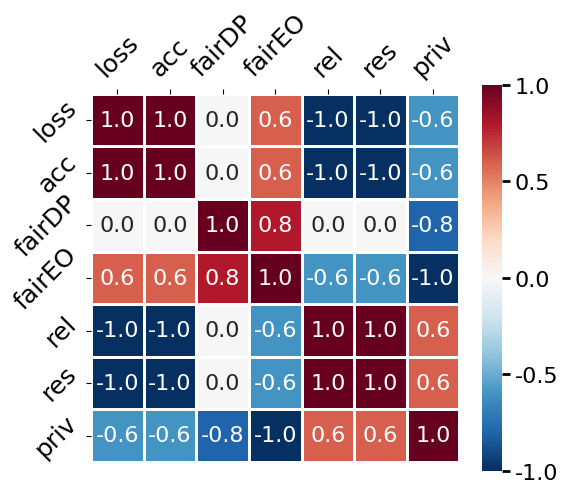
\includegraphics[width=\linewidth]{figs/H_4_A_N_l1o.png}
        \caption{Adult: 4 N / LOO}
    \end{subfigure}
    \hfill
    \begin{subfigure}{0.24\textwidth}
        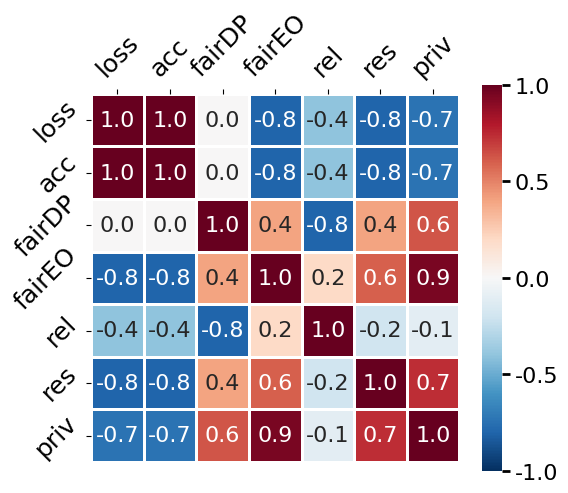
\includegraphics[width=\linewidth]{figs/H_4_A_N_gtg.png}
        \caption{Adult: 4 N / GTG}
    \end{subfigure}
    \hfill
    \begin{subfigure}{0.24\textwidth}
        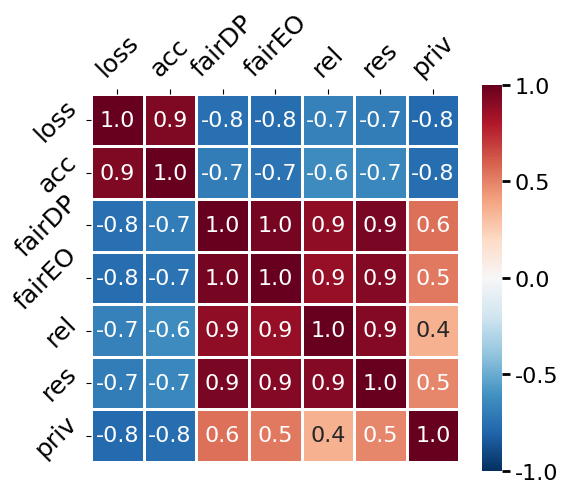
\includegraphics[width=\linewidth]{figs/H_20_A_N_l1o.png}
        \caption{Adult: 20 N / LOO}
    \end{subfigure}
    \hfill
    \begin{subfigure}{0.24\textwidth}
        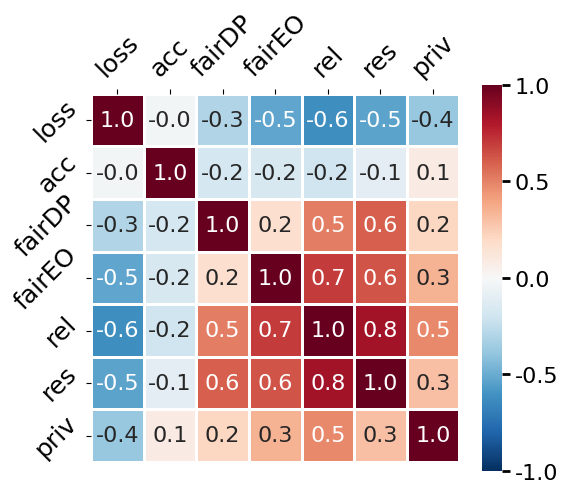
\includegraphics[width=\linewidth]{figs/H_20_A_N_gtg.png}
        \caption{Adult: 20 N / GTG}
    \end{subfigure}

    % CelebA - NIID
    \begin{subfigure}{0.24\textwidth}
        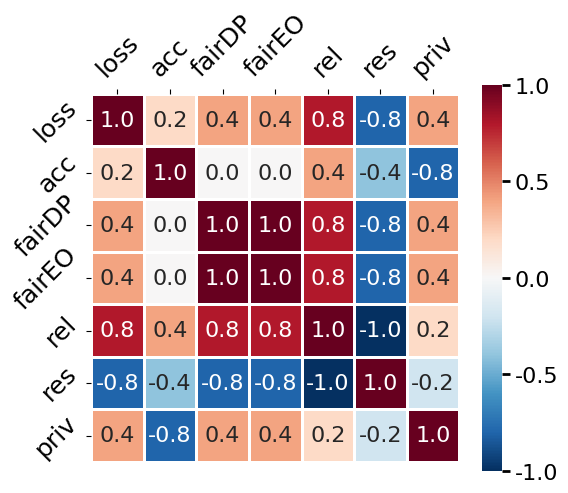
\includegraphics[width=\linewidth]{figs/H_4_C_N_l1o.png}
        \caption{CelebA: 4 N / LOO}
    \end{subfigure}
    \hfill
    \begin{subfigure}{0.24\textwidth}
        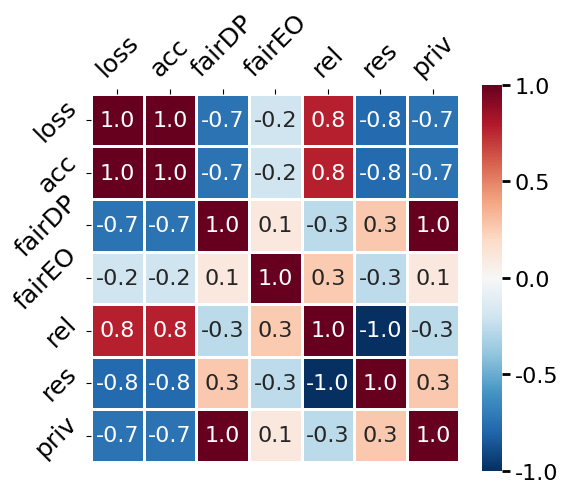
\includegraphics[width=\linewidth]{figs/H_4_C_N_gtg.png}
        \caption{CelebA: 4 N / GTG}
    \end{subfigure}
    \hfill
    \begin{subfigure}{0.24\textwidth}
        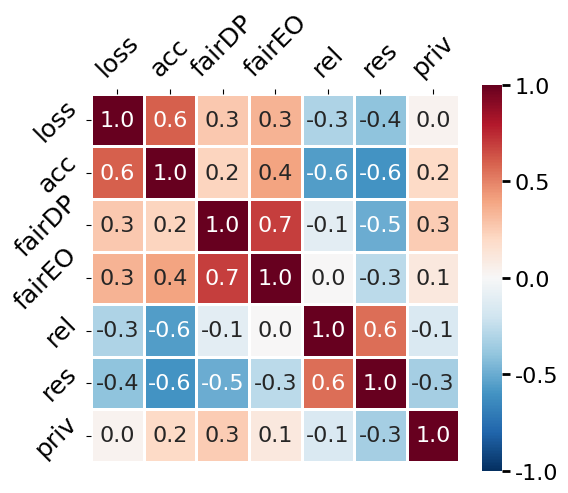
\includegraphics[width=\linewidth]{figs/H_20_C_N_l1o.png}
        \caption{CelebA: 20 N / LOO}
    \end{subfigure}
    \hfill
    \begin{subfigure}{0.24\textwidth}
        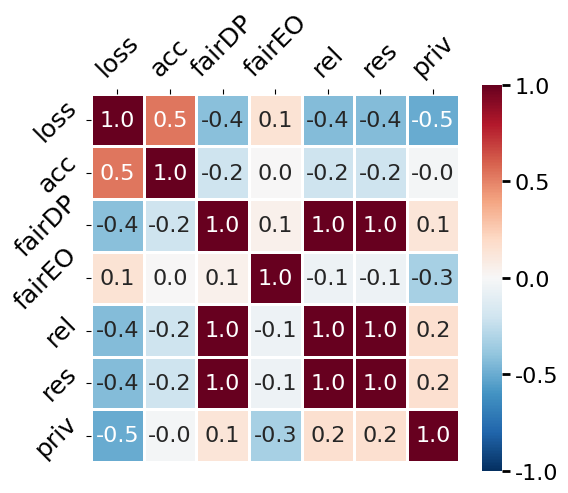
\includegraphics[width=\linewidth]{figs/H_20_C_N_gtg.png}
        \caption{CelebA: 20 N / GTG}
    \end{subfigure}

    % IMDB - NIID
    \begin{subfigure}{0.24\textwidth}
        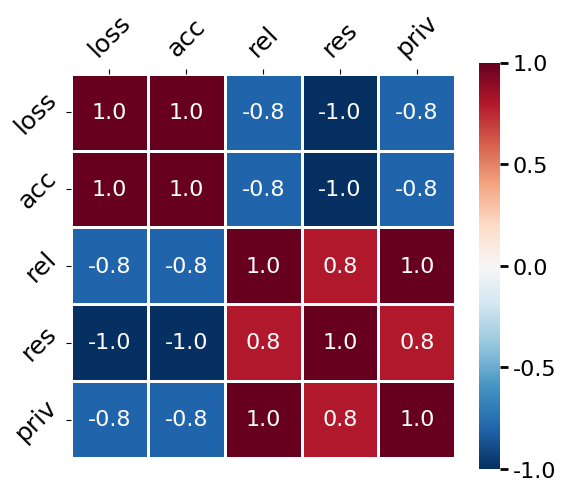
\includegraphics[width=\linewidth]{figs/H_4_I_N_l1o.png}
        \caption{IMDB: 4 N / LOO}
    \end{subfigure}
    \hfill
    \begin{subfigure}{0.24\textwidth}
        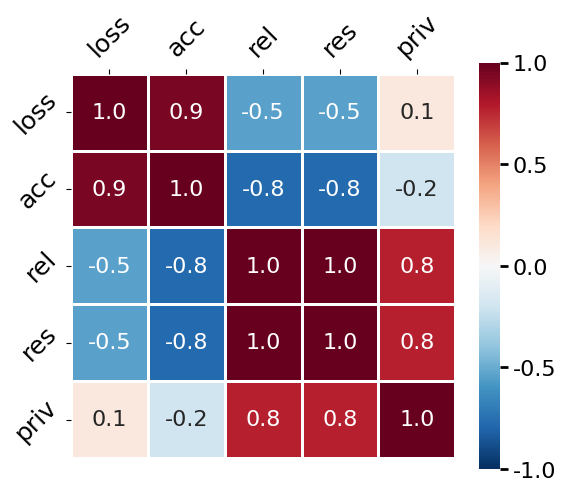
\includegraphics[width=\linewidth]{figs/H_4_I_N_gtg.png}
        \caption{IMDB: 4 N / GTG}
    \end{subfigure}
    \hfill
    \begin{subfigure}{0.24\textwidth}
        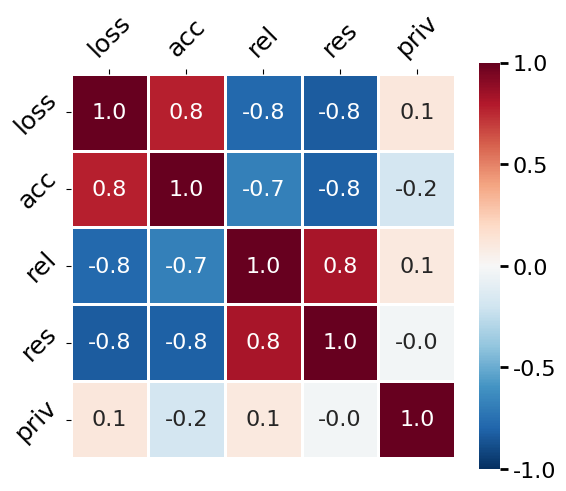
\includegraphics[width=\linewidth]{figs/H_20_I_N_l1o.png}
        \caption{IMDB: 20 N / LOO}
    \end{subfigure}
    \hfill
    \begin{subfigure}{0.24\textwidth}
        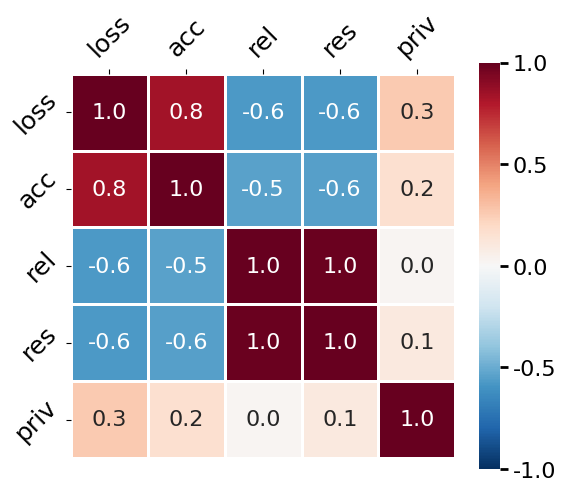
\includegraphics[width=\linewidth]{figs/H_20_I_N_gtg.png}
        \caption{IMDB: 20 N / GTG}
    \end{subfigure}
    
    \caption{Heatmap of the pair-wise score correlations (round $t=10$) for all non-IID scenarios. }
    \label{fig:score_heat_NIID}
\end{figure}

The key finding of this paper is presented in this table. As a sanity check, the accuracy contribution correlates positively with the loss baseline under both estimators in every non-degenerate setting, exactly as expected for two metrics that both capture predictive quality (the three near-zero GTG exceptions --- ADULT $-0.20$ at IID $K{=}4$, ADULT $-0.03$ at non-IID $K{=}20$, and CelebA $-0.20$ at IID $K{=}4$ --- stem from nearly equal contributions whose ranking is dominated by noise). The trustworthiness scores behave oppositely under non-IID partitioning: at $K{=}20$, reliability and resilience turn negative against the loss baseline for all three datasets under both estimators (down to $\Phi=-0.83$ for IMDB resilience under LOO), while on ADULT every trustworthiness dimension inverts ($\Phi\le-0.68$ under LOO), most pronounced for privacy ($-0.78$); for fairness and privacy the effect is dataset-dependent. GTG, acting as a variance dampener, generally mutes these negative correlations toward zero. Such negative correlations expose a systemic risk: the clients driving the largest gains in predictive performance can simultaneously be the most detrimental to the model's other trustworthiness dimensions. The accompanying $L_2$ differences confirm that these are not mere ranking artifacts but substantial numerical gaps in valuation, which matters directly whenever contributions are translated into monetary rewards. Together, these results show that evaluating participants through a single performance metric is inadequate for any consortium that values trustworthiness; every dimension of interest must be measured and governed explicitly.

\subsection{Score Utilization}

\subsubsection*{Setup}

Having established that client contributions vary drastically across different trustworthiness dimensions, we now transition from passive evaluation to active intervention. The standard Federated Averaging algorithm aggregates local models based strictly on the size of a client's local dataset. This aggregation implicitly assumes that data quantity equals data quality, completely ignoring the multifaceted trustworthiness of the updates. To actively steer the global model toward a specific trustworthy objective, we introduce a client reweighting mechanism. Rather than solely using dataset sizes, we also utilize the obtained scores inspired by~\cite{velez2026private}. To ensure numerical stability, the raw scores ($\mathtt{CS}_v(D_k)$) are first shifted to be strictly positive ($\mathtt{CS}^\prime_v(D_k)=\mathtt{CS}_v(D_k) + |\min_k\{0, \mathtt{CS}_v(D_k)\}|$) and then normalized by their mean, i.e., $\mathtt{CS}^{\prime\prime}_v(D_k)=\mathtt{CS}^\prime_v(D_k)/\text{avg}_k\{\mathtt{CS}^\prime_v(D_k)\}$. This yields weights that hover around $1$. Finally, each weight is clipped to the range $[0.5, 2]$, so no single client can dominate the aggregate regardless of the score distribution. This mechanism systematically amplifies the influence of clients who improve the targeted trustworthiness dimension while diminishing those who degrade it. To isolate and thoroughly evaluate the efficacy of this score-based intervention, we design four distinct aggregation scenarios. 

\begin{itemize}
    \item \textbf{Baseline (BL):} The standard performance-centric aggregation relying solely on dataset sizes.
    \item \textbf{Static Weighting (ST):} The scores are computed exclusively at round $t=2$. The resulting scores are transformed into weights as described above, then fixed and utilized for the remainder of the training.
    \item \textbf{Dynamic Weighting (DY):} Trustworthiness scores are recomputed in every round $t\geq2$, and the round-$t$ aggregation weights are derived solely from that round's fresh scores via the same transformation. Recomputing from fresh scores --- rather than multiplicatively updating an accumulated score --- avoids double-counting persistently strong or weak clients across rounds.
    \item \textbf{Explicit Training (ET):} Clients explicitly modify their local training processes to include trustworthy constraints.
\end{itemize}

To benchmark our weightings against explicit local interventions, we implement three standard techniques covering the evaluated trustworthiness spectrum: fairness regularization, adversarial training, and differential privacy. To promote fairness, clients augment their local loss functions with a Demographic Parity regularization penalty, scaled by a coefficient $\lambda = 2.0$. To achieve empirical robustness, clients adopt standard adversarial training~\cite{madry2017towards}, replacing $50\%$ of their clean local batches ($100\%$ for CelebA and IMDB) with PGD-perturbed examples. These adversarial samples are generated using the per-dataset training bounds $\varepsilon$ and step sizes $\alpha$ ($\alpha=0.007, \varepsilon=0.3$ for ADULT; $\alpha=0.007, \varepsilon=0.03$ for CelebA; $\alpha=0.00125, \varepsilon=0.005$ for IMDB; note that the CelebA defense is trained at the standard $\varepsilon=0.03$ while its resilience is evaluated at the smaller $\varepsilon=0.01$), paired with $7$ attack steps during training ($10$ for CelebA and IMDB, following Madry et al.~\cite{madry2017towards}, who reserve longer iteration counts for evaluation only). Finally, to provide formal privacy guarantees, clients train their local models using Differentially Private SGD (DP-SGD)~\cite{abadi2016deep}, utilizing a gradient clipping norm of $C = 1.0$ and a noise multiplier of $\sigma_{\text{DP}} = 1.0$.

\subsubsection*{Results}

\begin{table}[!t]
    \centering
    \resizebox{0.9\linewidth}{!}{
    \setlength{\tabcolsep}{2pt}
\begin{tabular}{cc||cc|cc|cc|}
    \multicolumn{2}{c||}{\multirow{2}{*}{\textbf{Setting}}}
    & \multicolumn{2}{c|}{\textbf{$\mathtt{ADULT}$}}
    & \multicolumn{2}{c|}{\textbf{$\mathtt{CelebA}$}}
    & \multicolumn{2}{c|}{\textbf{$\mathtt{IMDB}$}} \\
    && $4$ & $20$ & $4$ & $20$ & $4$ & $20$ \\
    \hline\hline
    \multirow{3}{*}{$\mathtt{loss}$}
    & BL & $0.71 \pm 0.03$ & $0.69 \pm 0.02$ & $0.79 \pm 0.01$ & $0.80 \pm 0.00$ & $0.74 \pm 0.00$ & $0.74 \pm 0.00$ \\
    & ST & $0.73 \pm 0.01$ & $0.72 \pm 0.01$ & $0.79 \pm 0.02$ & $0.81 \pm 0.01$ & $0.76 \pm 0.00$ & $0.74 \pm 0.00$ \\
    & DY & $0.73 \pm 0.01$ & $0.72 \pm 0.01$ & $0.79 \pm 0.03$ & $0.81 \pm 0.00$ & $0.76 \pm 0.00$ & $0.74 \pm 0.00$ \\
    \hline
    \multirow{3}{*}{$\mathtt{acc}$}
    & BL & $0.85 \pm 0.01$ & $0.84 \pm 0.01$ & $0.91 \pm 0.00$ & $0.91 \pm 0.00$ & $0.87 \pm 0.00$ & $0.87 \pm 0.00$ \\
    & ST & $0.85 \pm 0.01$ & $0.84 \pm 0.01$ & $0.91 \pm 0.01$ & $0.91 \pm 0.01$ & $0.89 \pm 0.00$ & $0.86 \pm 0.00$ \\
    & DY & $0.85 \pm 0.03$ & $0.84 \pm 0.01$ & $0.89 \pm 0.03$ & $0.91 \pm 0.00$ & $0.89 \pm 0.01$ & $0.87 \pm 0.00$ \\
    \hline\hline
    Fair. Reg.& ET & $0.92 \pm 0.03$ & $0.94 \pm 0.02$ & $0.97 \pm 0.03$ & $0.96 \pm 0.02$ & -- & -- \\
    % ET-fair on fairEO: $0.96 \pm 0.02$ & $0.96 \pm 0.01$ & $0.96 \pm 0.03$ & $0.96 \pm 0.02$ & -- & --
    \hline
    \multirow{3}{*}{$\mathtt{fairDP}$}
    & BL & $0.88 \pm 0.04$ & $0.90 \pm 0.02$ & $0.87 \pm 0.01$ & $0.87 \pm 0.01$ & -- & -- \\
    & ST & $0.93 \pm 0.06$ & $0.95 \pm 0.01$ & $0.86 \pm 0.02$ & $0.83 \pm 0.01$ & -- & -- \\
    & DY & $0.92 \pm 0.06$ & $0.93 \pm 0.04$ & $0.87 \pm 0.03$ & $0.84 \pm 0.00$ & -- & -- \\
    \hline
    \multirow{3}{*}{$\mathtt{fairEO}$}
    & BL & $0.96 \pm 0.03$ & $0.96 \pm 0.02$ & $0.98 \pm 0.01$ & $0.98 \pm 0.01$ & -- & -- \\
    & ST & $0.97 \pm 0.03$ & $0.99 \pm 0.01$ & $0.97 \pm 0.02$ & $0.97 \pm 0.01$ & -- & -- \\
    & DY & $0.97 \pm 0.03$ & $0.97 \pm 0.03$ & $0.98 \pm 0.00$ & $0.98 \pm 0.01$ & -- & -- \\
    \hline\hline
    Rob. Train.& ET & $0.77 \pm 0.08$ & $0.73 \pm 0.20$ & $0.88 \pm 0.01$ & $0.92 \pm 0.00$ & $0.84 \pm 0.00$ & $0.85 \pm 0.00$ \\
    % ET-adv on rel: $0.99 \pm 0.00$ & $0.99 \pm 0.00$ & $0.98 \pm 0.00$ & $0.98 \pm 0.00$ & $0.72 \pm 0.00$ & $0.75 \pm 0.00$
    \hline
    \multirow{3}{*}{$\mathtt{rel}$}
    & BL & $0.99 \pm 0.00$ & $0.99 \pm 0.00$ & $0.91 \pm 0.01$ & $0.91 \pm 0.02$ & $0.74 \pm 0.00$ & $0.76 \pm 0.00$ \\
    & ST & $0.99 \pm 0.00$ & $0.99 \pm 0.00$ & $0.93 \pm 0.03$ & $0.87 \pm 0.03$ & $0.76 \pm 0.01$ & $0.76 \pm 0.00$ \\
    & DY & $0.99 \pm 0.00$ & $0.99 \pm 0.00$ & $0.91 \pm 0.03$ & $0.91 \pm 0.02$ & $0.77 \pm 0.01$ & $0.76 \pm 0.00$ \\
    \hline
    \multirow{3}{*}{$\mathtt{res}$}
    & BL & $0.48 \pm 0.06$ & $0.63 \pm 0.07$ & $0.52 \pm 0.01$ & $0.53 \pm 0.02$ & $0.41 \pm 0.01$ & $0.48 \pm 0.01$ \\
    & ST & $0.65 \pm 0.13$ & $0.86 \pm 0.05$ & $0.75 \pm 0.06$ & $0.61 \pm 0.03$ & $0.50 \pm 0.06$ & $0.49 \pm 0.00$ \\
    & DY & $0.68 \pm 0.16$ & $0.85 \pm 0.05$ & $0.83 \pm 0.06$ & $0.63 \pm 0.02$ & $0.45 \pm 0.03$ & $0.50 \pm 0.01$ \\
    \hline\hline
    Diff. Priv.& ET & $0.97 \pm 0.01$ & $0.97 \pm 0.00$ & $0.96 \pm 0.02$ & $0.95 \pm 0.01$ & $0.91 \pm 0.01$ & $0.94 \pm 0.01$ \\
    \hline
    \multirow{3}{*}{$\mathtt{priv}$}
    & BL & $0.93 \pm 0.03$ & $0.96 \pm 0.02$ & $0.90 \pm 0.03$ & $0.93 \pm 0.03$ & $0.84 \pm 0.01$ & $0.88 \pm 0.02$ \\
    & ST & $0.92 \pm 0.02$ & $0.92 \pm 0.01$ & $0.95 \pm 0.02$ & $0.94 \pm 0.02$ & $0.83 \pm 0.04$ & $0.91 \pm 0.04$ \\
    & DY & $0.93 \pm 0.02$ & $0.94 \pm 0.02$ & $0.93 \pm 0.03$ & $0.94 \pm 0.02$ & $0.84 \pm 0.04$ & $0.89 \pm 0.02$ \\
    \hline
    \end{tabular}    }
    \caption{Final global-model scores under GTG-based reweighting of non-IID clients. BL is the standard dataset-size baseline, ST applies weights computed at round $t=2$, and DY recomputes weights every round. The ET rows represent explicit local training of the matching constraint (Demographic-Parity regularization, adversarial training, and DP-SGD). Higher values indicate better performance across all metrics.}
    \label{tab:util}
\end{table}

Because the various dimensions of trustworthiness inherently conflict, attempting to visualize all interventions simultaneously obfuscates the underlying dynamics. Therefore, we evaluate our reweighting mechanism on each trustworthiness pillar in isolation (Tab.~\ref{tab:util}). 

Our server-side reweighting steers the global model along the targeted dimension without clients altering their local code or seeing a single adversarial example. Resilience is the clearest case: on ADULT at $K=20$ it climbs from $0.63$ to $0.86$, surpassing even explicit adversarial training ($0.73$) in that setting; on CelebA at $K=4$ it climbs from $0.52$ to $0.83$, though explicit adversarial training ($0.88$) stays ahead there. The gain is notable because it comes purely from amplifying clients whose data already yields flatter, more robust loss landscapes, with no adversarial exposure during local training. Reweighting isolates and amplifies these naturally robust updates, side-stepping the local non-convergence that explicit adversarial training can suffer. On ADULT, our fairness weighting reaches parity with a well-tuned Demographic-Parity regularization baseline (fairDP $0.95$ vs.\ $0.94$ at $K=20$); on CelebA it does not improve over the size baseline, so parity is dataset-dependent.

Comparing the two weighting schemes, Dynamic Weighting reaches the highest absolute peaks on several dimensions but does so with larger seed-to-seed variance and an immense computational cost, since it demands a fresh Shapley approximation every round. Static Weighting, computed once at round two, captures most of the benefit at a fraction of the cost, making it the more practical choice for deployment. We also note that several dimensions leave little room to improve: where the baseline already sits near the ceiling, reweighting changes little, simply because no client subset is meaningfully degrading that dimension to begin with. For privacy in particular, explicit DP-SGD remains the stronger lever, as expected from a mechanism with formal guarantees.

Finally, the intervention makes the trade-offs from our correlation analysis concrete. Because the weights multiplicatively favor clients who boost the targeted dimension, they necessarily de-prioritize the clients whose data most improves predictive quality. The cost to predictive accuracy is modest on these datasets: across the reweighting schemes the accuracy block stays within roughly $0.02$ of the size baseline, since the clipped weights hover around $1$ and cannot fully suppress the performance-driving clients. The effect is real but bounded and it reinforces our central message: trustworthiness in federated systems is not a free by-product of collaboration but a distinct objective that demands deliberate, quantifiable, and sometimes costly trade-offs.

\section{Conclusion}
\label{sec:con}

Our investigation demonstrates that evaluating clients in Federated Learning solely through standard performance objectives (e.g., minimizing loss) provides an incomplete, and often highly misleading, picture of their true systemic contribution. By extending client evaluation to encompass a multi-dimensional spectrum of trustworthiness (fairness, robustness, and privacy), we reveal that a client's value is fundamentally context-dependent and heavily influenced by the underlying data distribution. 

Our empirical results in non-IID scenarios show that performance-wise "good" clients are not necessarily trustworthy. In fact, pairwise correlation analysis exposes strict operational trade-offs: the specific clients whose unique data shards drive the greatest improvements in global predictive accuracy are frequently the same clients introducing the highest privacy leakage risks or degrading model fairness. These findings have profound implications for federated governance and incentive design: a reward system based strictly on accuracy will frequently penalize the very clients who are essential for ensuring equitable and robust operation. Future work must explore how these multi-dimensional, sometimes conflicting scores can be integrated into a unified, holistic reward allocation scheme that prioritizes the deployment of truly dependable AI systems.

\subsubsection*{Limitations \& Future Work}

While our multi-dimensional framework provides a deeper diagnostic view of federated systems, it introduces substantial computational overhead. Exact client contribution evaluation via permutation-based methods like GTG-Shapley is notoriously NP-hard, creating an extreme computational bottleneck that strictly limits our empirical evaluation to smaller federations ($K \le 20$). Evaluating multiple trustworthiness metrics across every client round at massive scale currently remains intractable. Although our temporal stability analysis (Tab.~\ref{tab:score_fluct}) suggests that single-round evaluations may suffice for certain stable metrics (e.g., standard tabular fairness), highly fragmented data still requires multi-round accumulation for accurate scoring. Developing computationally lightweight proxies for these trustworthy dimensions remains a critical hurdle for real-world deployment. Furthermore, our choice of any single metric represents just one of many possibilities. We hypothesize that substituting these underlying definitions (such as utilizing alternative fairness definitions, different noise distributions, or alternative adversarial attacks) would result in subtle but meaningful shifts in individual client valuations. Finally, future research should investigate how these contribution scores evolve when trustworthiness is explicitly optimized during the federated training process itself (such as applying robust adversarial training or fairness regularization), as these active interventions would fundamentally alter the marginal value of each client's local data.

\begin{acks}
    \small
    Project no. 145832, implemented with the support provided by the Ministry of Innovation and Technology from the NRDI Fund, financed under the PD\_23 funding scheme.
\end{acks}

\bibliographystyle{ACM-Reference-Format}
\bibliography{ref}

\appendix

%\section{Client's Scores with $K=20$}

\begin{figure}[!t]
    \centering
    
    \begin{subfigure}{0.8\linewidth}
        \centering
        
\includegraphics[width=\linewidth]{figs/S_legend.png}
    \end{subfigure}

    \caption{Computed contribution scores (accumulated across rounds) for the $K=20$ client scenario; [A], [C], and [I] are ADULT, CelebA. and IMDB, while I and N denote IID and non-IID. }
    
    % ADULT - 20 Clients
    \begin{subfigure}{0.24\linewidth}
        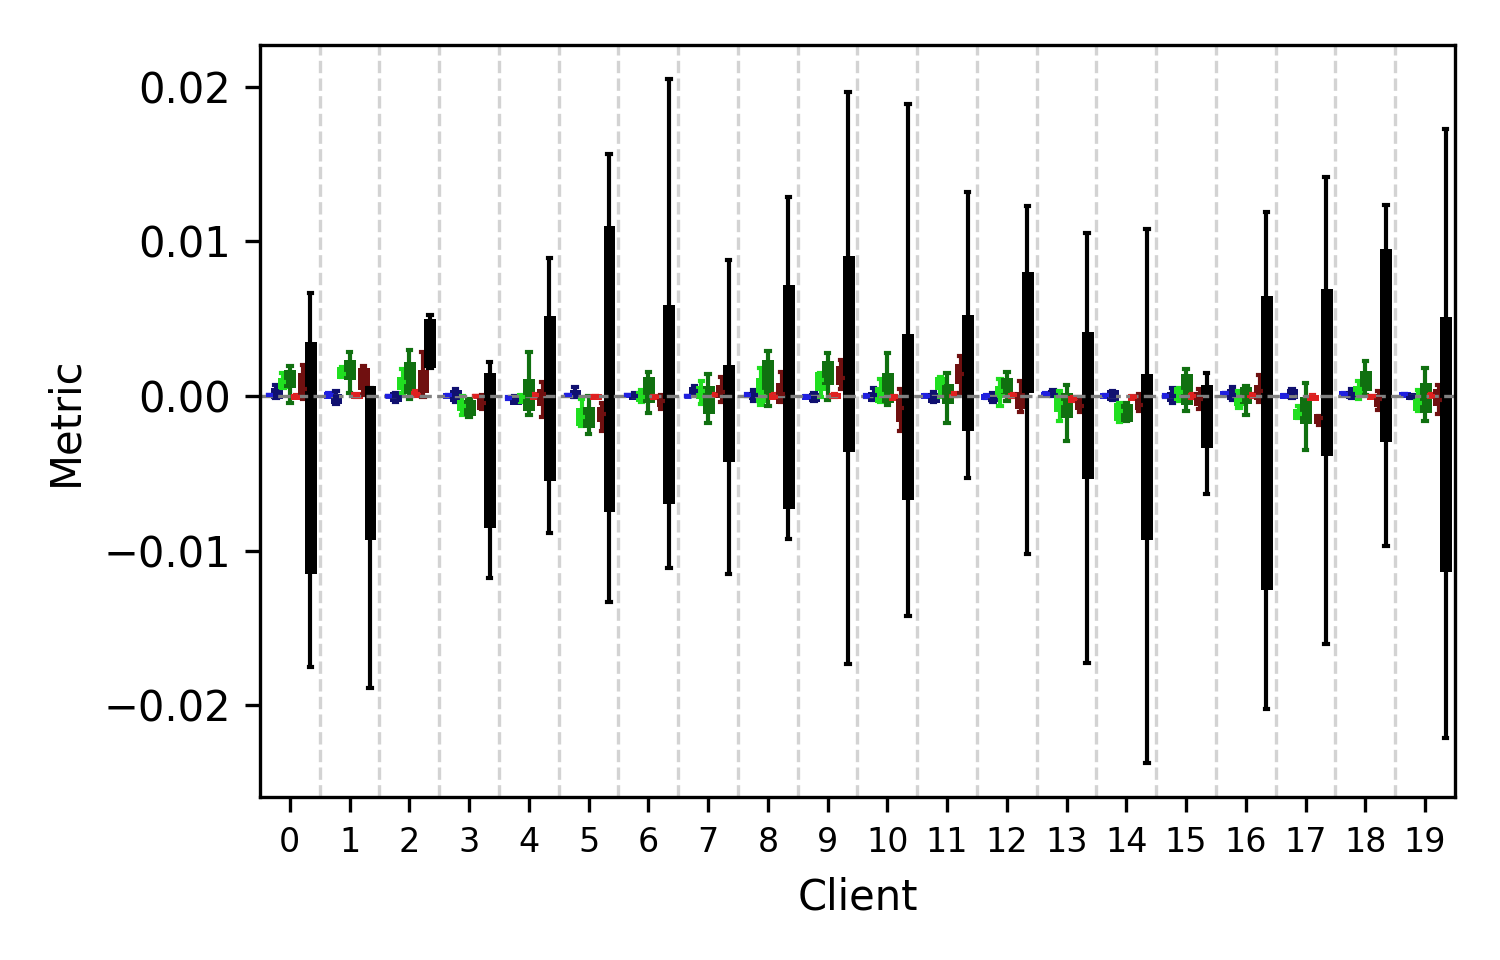
\includegraphics[width=\linewidth]{figs/S_A_20_I_l1o.png}
        \caption{[A]: 20 I / LOO}
    \end{subfigure}
    \hfill
    \begin{subfigure}{0.24\linewidth}
        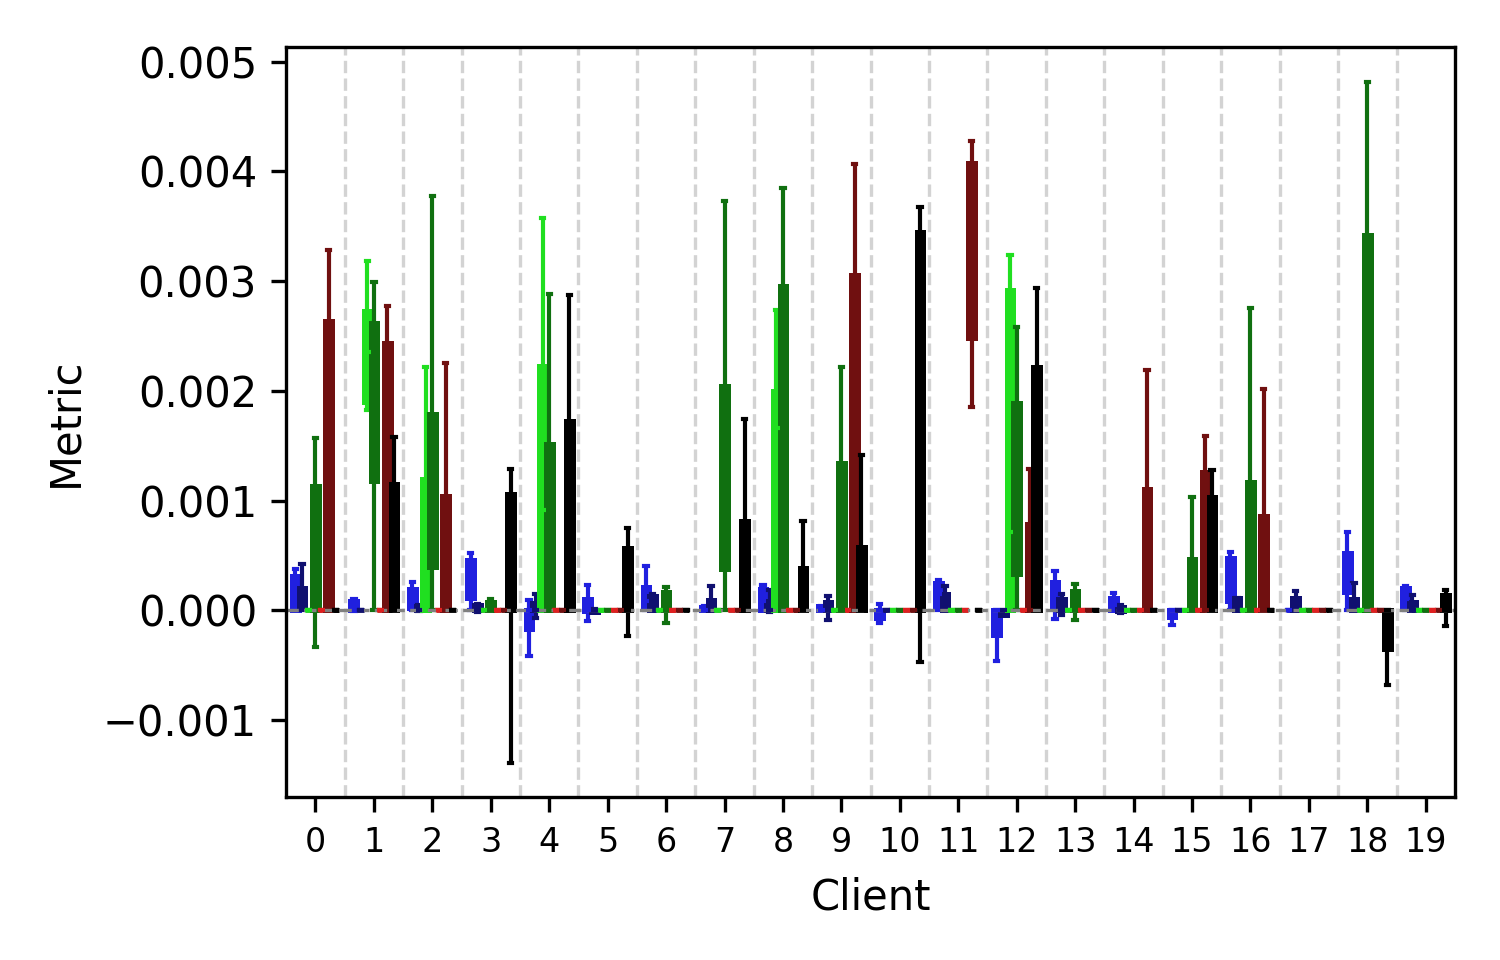
\includegraphics[width=\linewidth]{figs/S_A_20_I_gtg.png}
        \caption{[A]: 20 I / GTG}
    \end{subfigure}
    \hfill
    \begin{subfigure}{0.24\linewidth}
        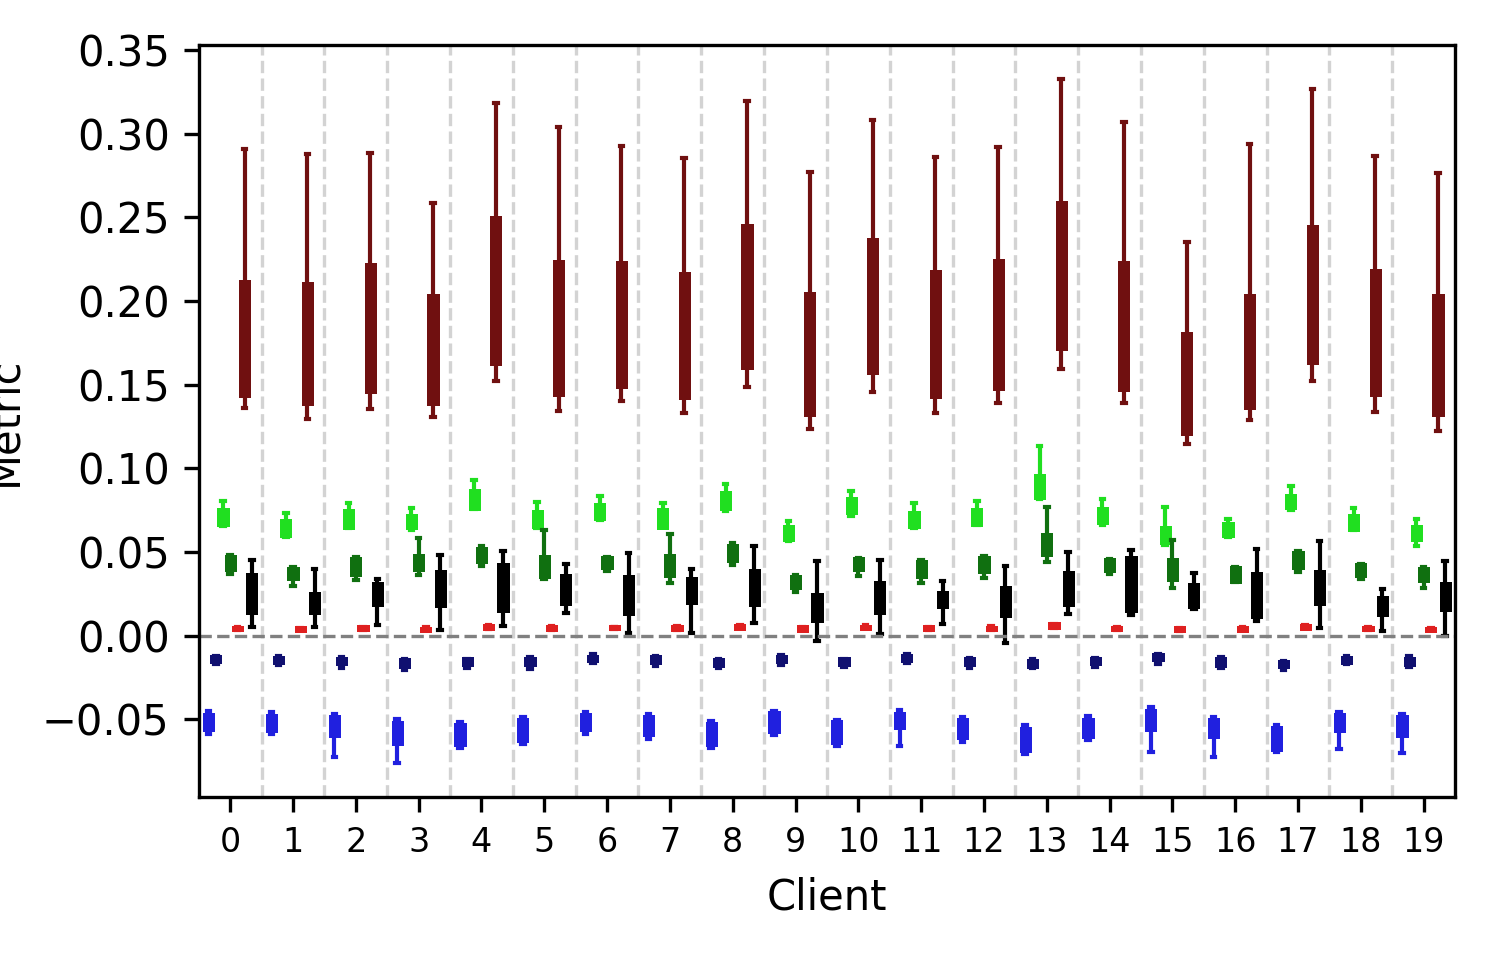
\includegraphics[width=\linewidth]{figs/S_A_20_N_l1o.png}
        \caption{[A]: 20 N / LOO}
    \end{subfigure}
    \hfill
    \begin{subfigure}{0.24\linewidth}
        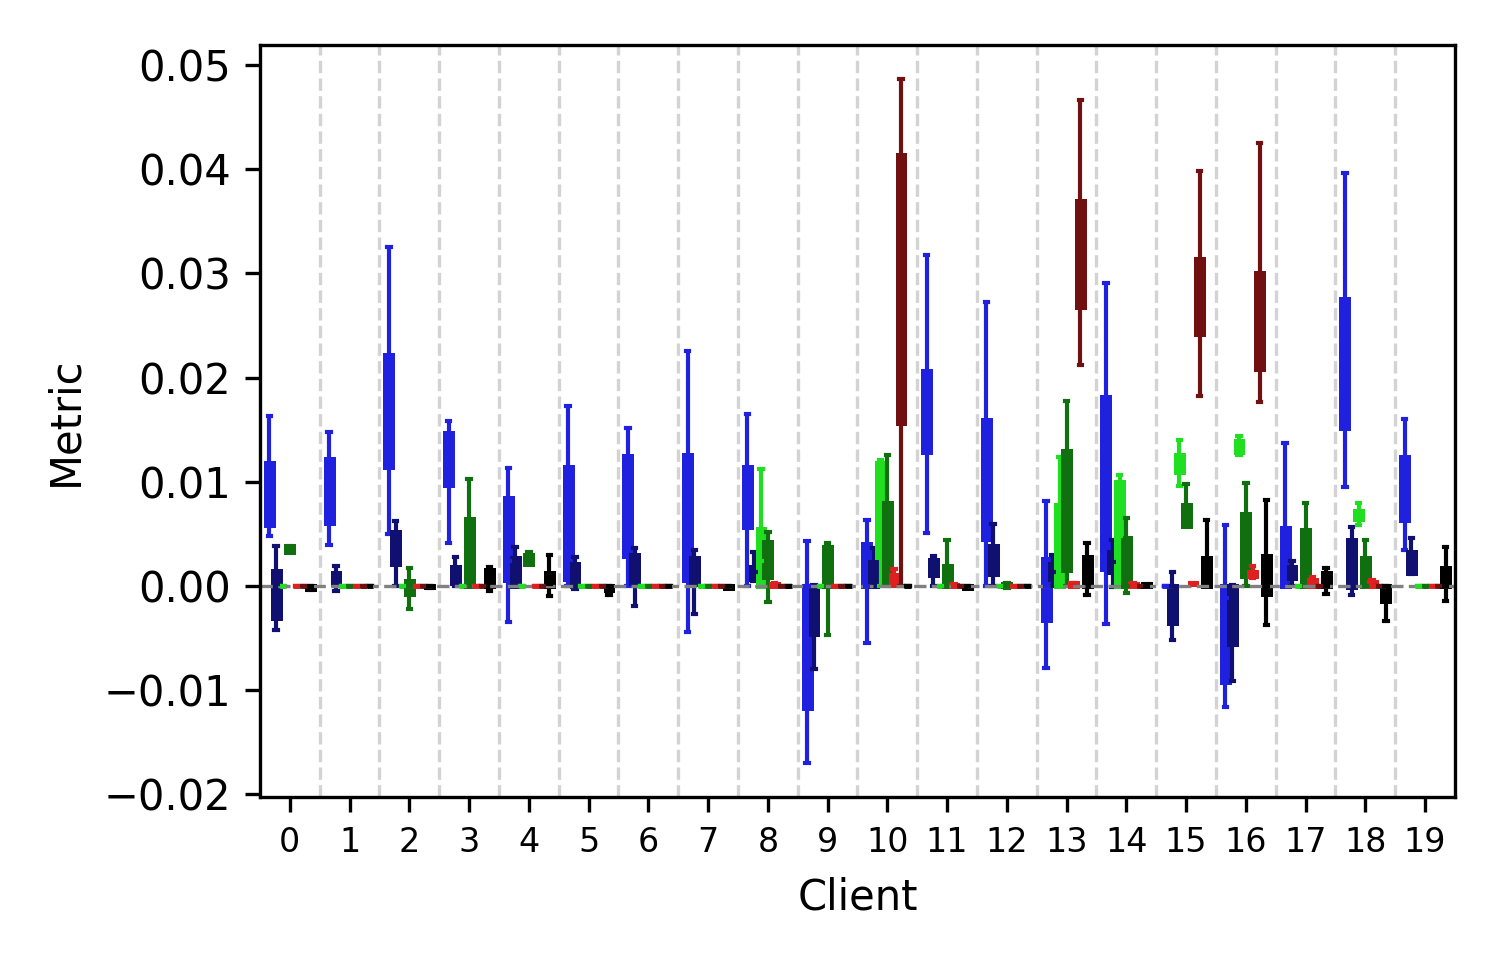
\includegraphics[width=\linewidth]{figs/S_A_20_N_gtg.png}
        \caption{[A]: 20 N / GTG}
    \end{subfigure}

    % CelebA - 20 Clients
    \begin{subfigure}{0.24\linewidth}
        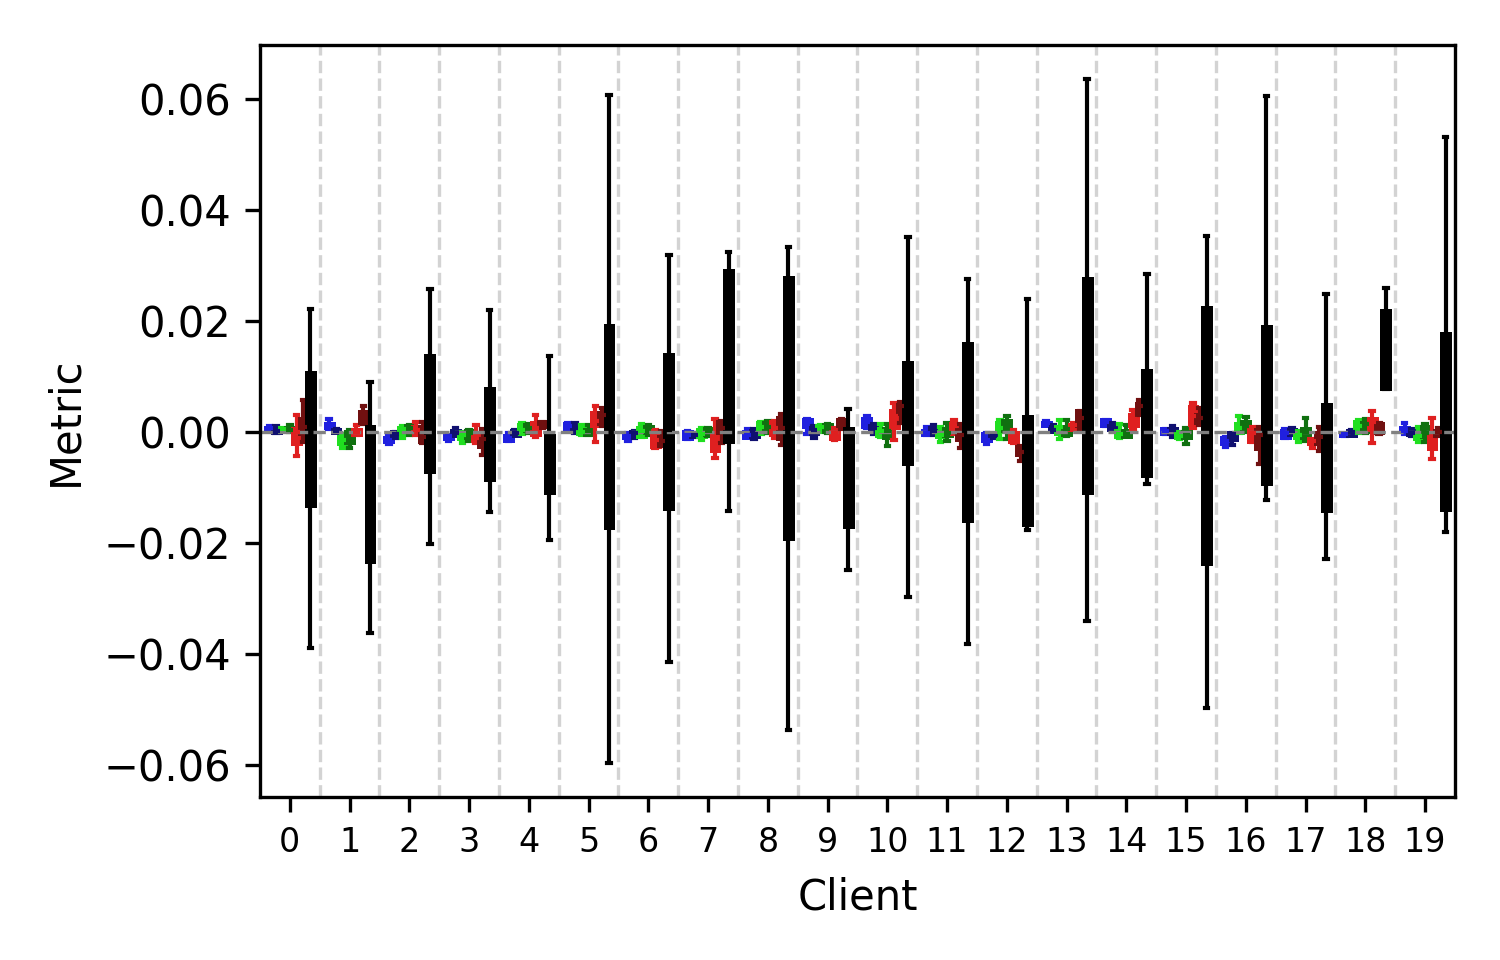
\includegraphics[width=\linewidth]{figs/S_C_20_I_l1o.png}
        \caption{[C]: 20 I / LOO}
    \end{subfigure}
    \hfill
    \begin{subfigure}{0.24\linewidth}
        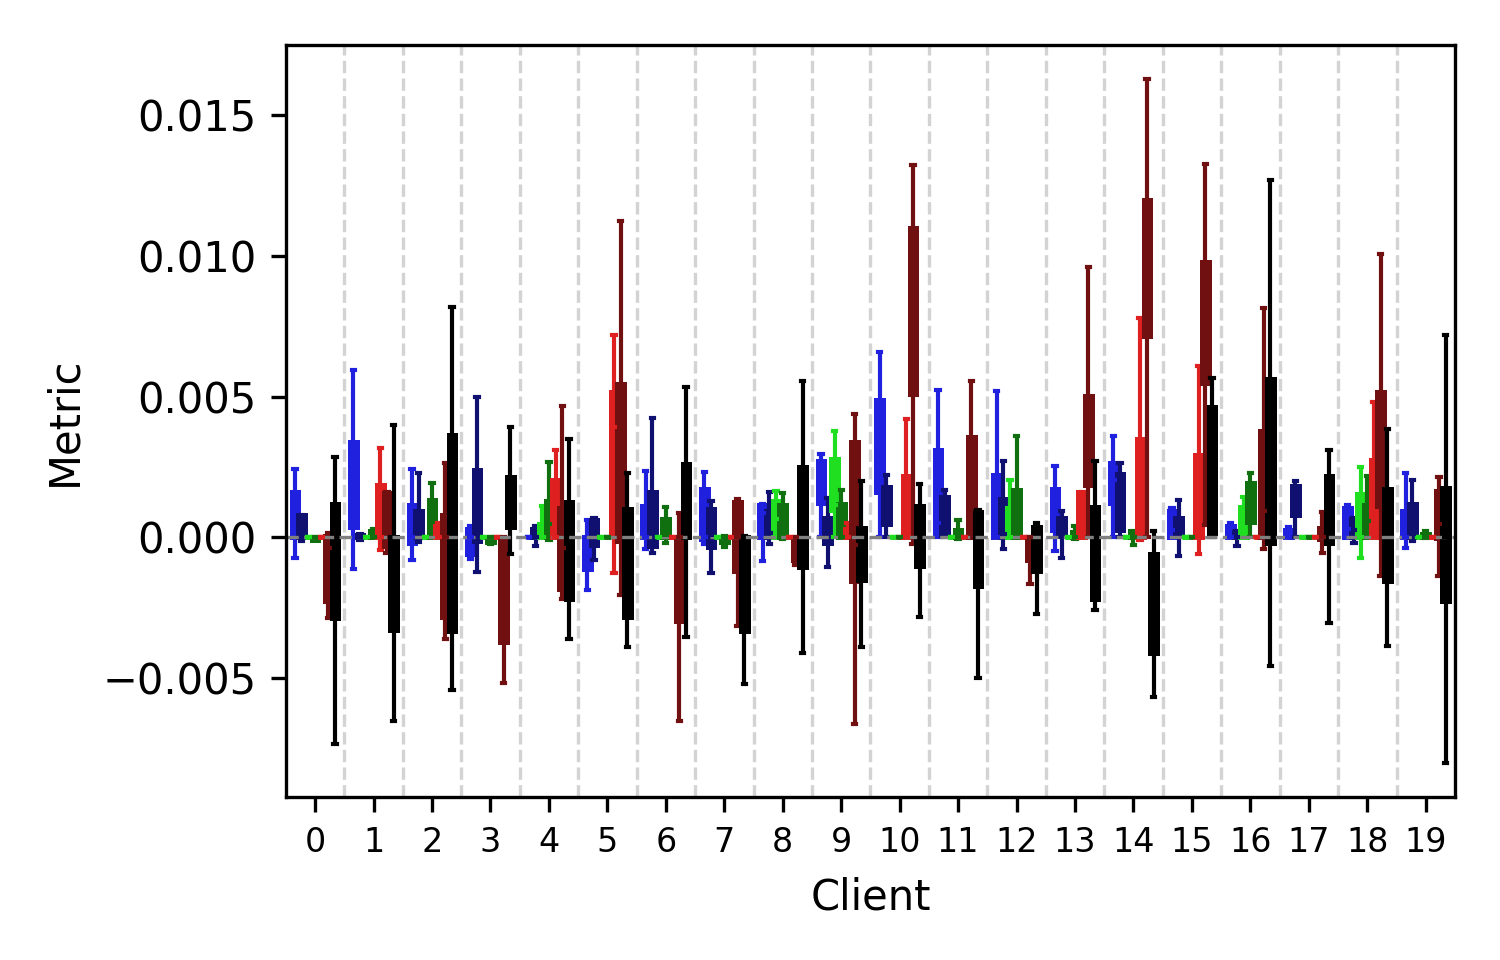
\includegraphics[width=\linewidth]{figs/S_C_20_I_gtg.png}
        \caption{[C]: 20 I / GTG}
    \end{subfigure}
    \hfill
    \begin{subfigure}{0.24\linewidth}
        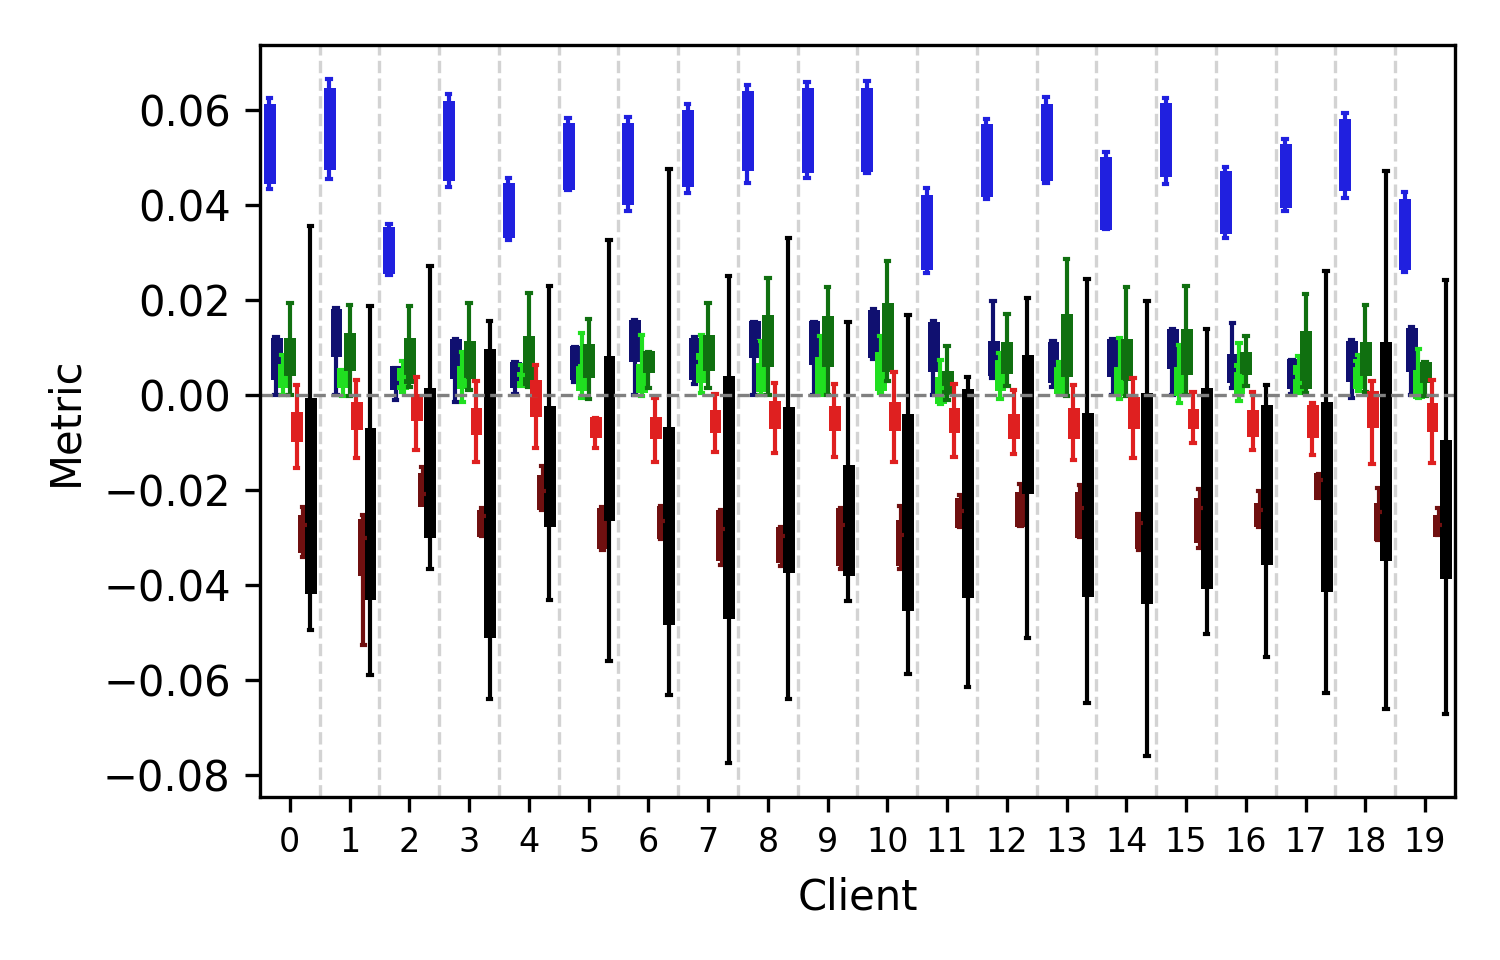
\includegraphics[width=\linewidth]{figs/S_C_20_N_l1o.png}
        \caption{[C]: 20 N / LOO}
    \end{subfigure}
    \hfill
    \begin{subfigure}{0.24\linewidth}
        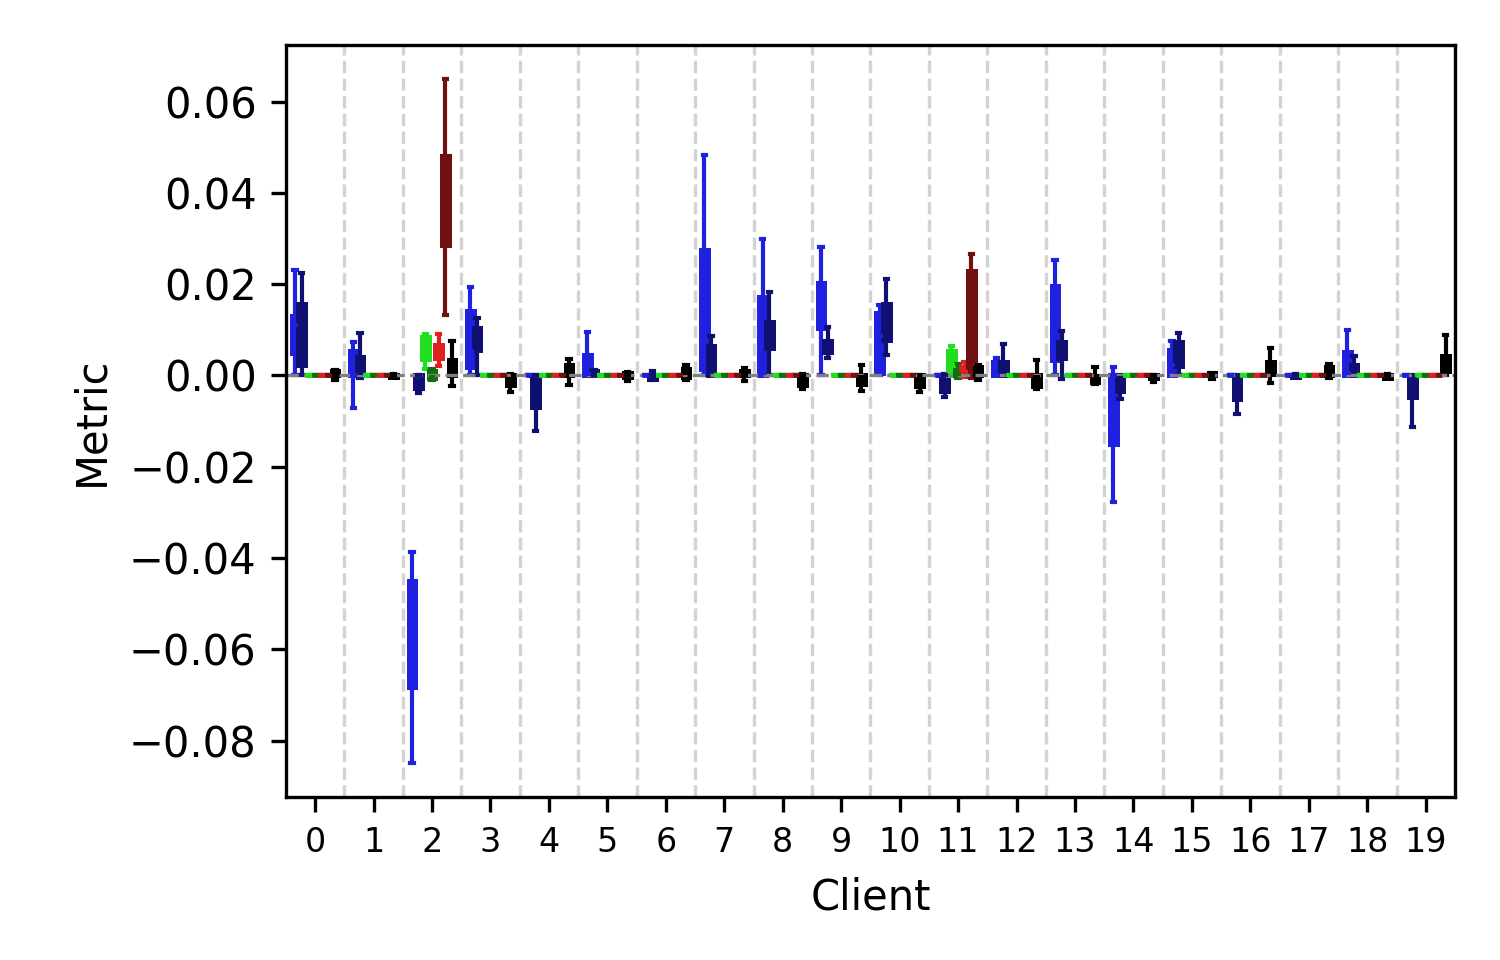
\includegraphics[width=\linewidth]{figs/S_C_20_N_gtg.png}
        \caption{[C]: 20 N / GTG}
    \end{subfigure}

    % IMDB - 20 Clients
    \begin{subfigure}{0.24\linewidth}
        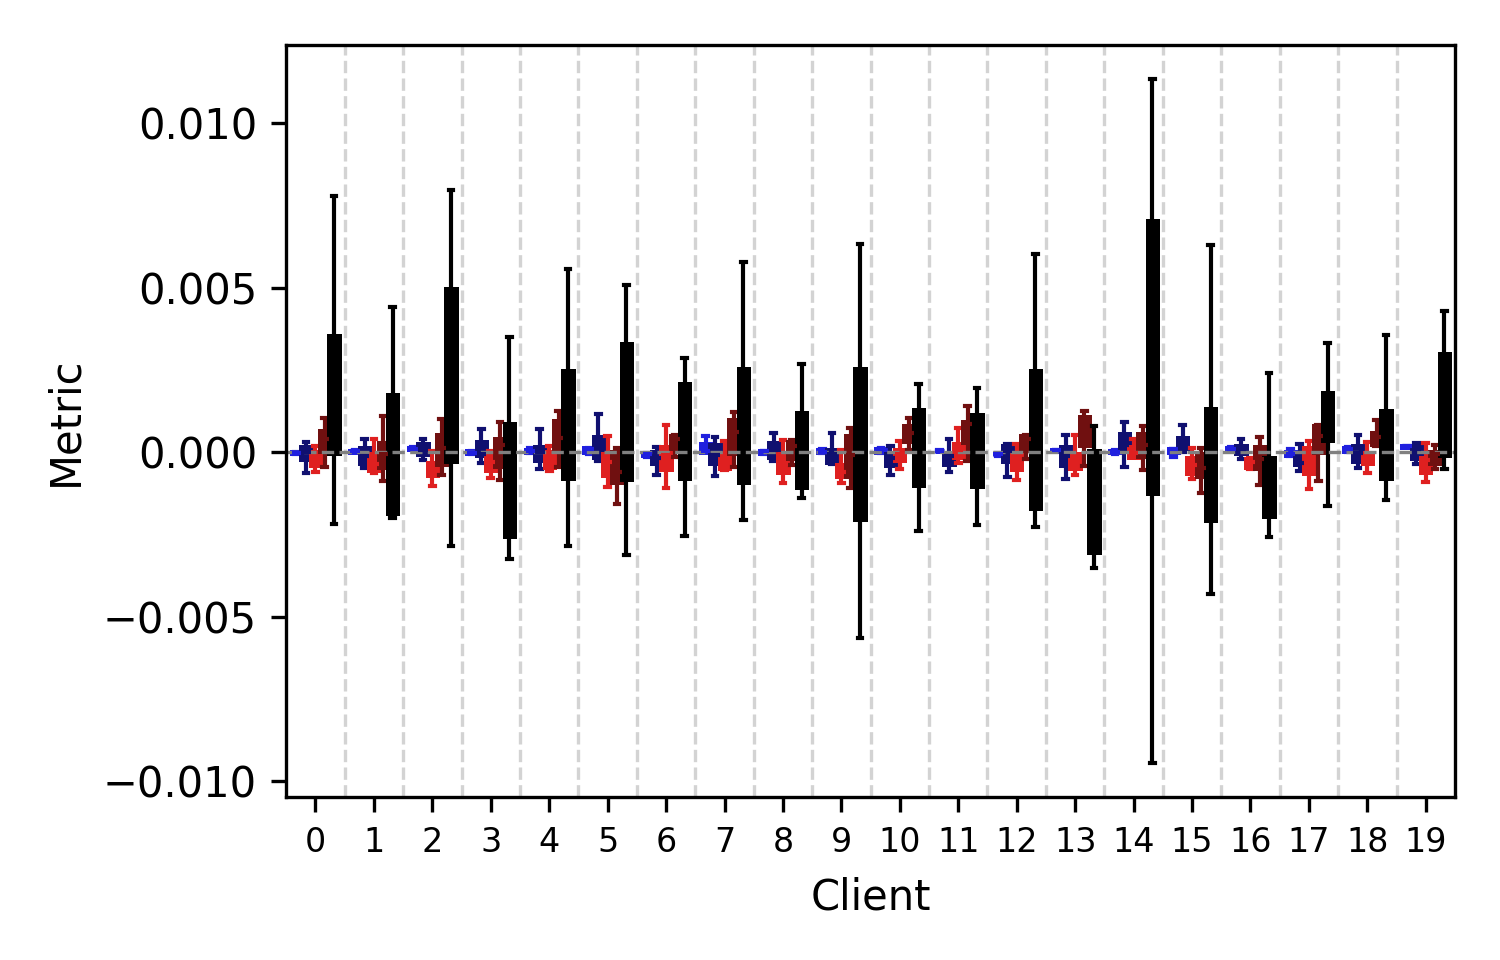
\includegraphics[width=\linewidth]{figs/S_I_20_I_l1o.png}
        \caption{[I]: 20 I / LOO}
    \end{subfigure}
    \hfill
    \begin{subfigure}{0.24\linewidth}
        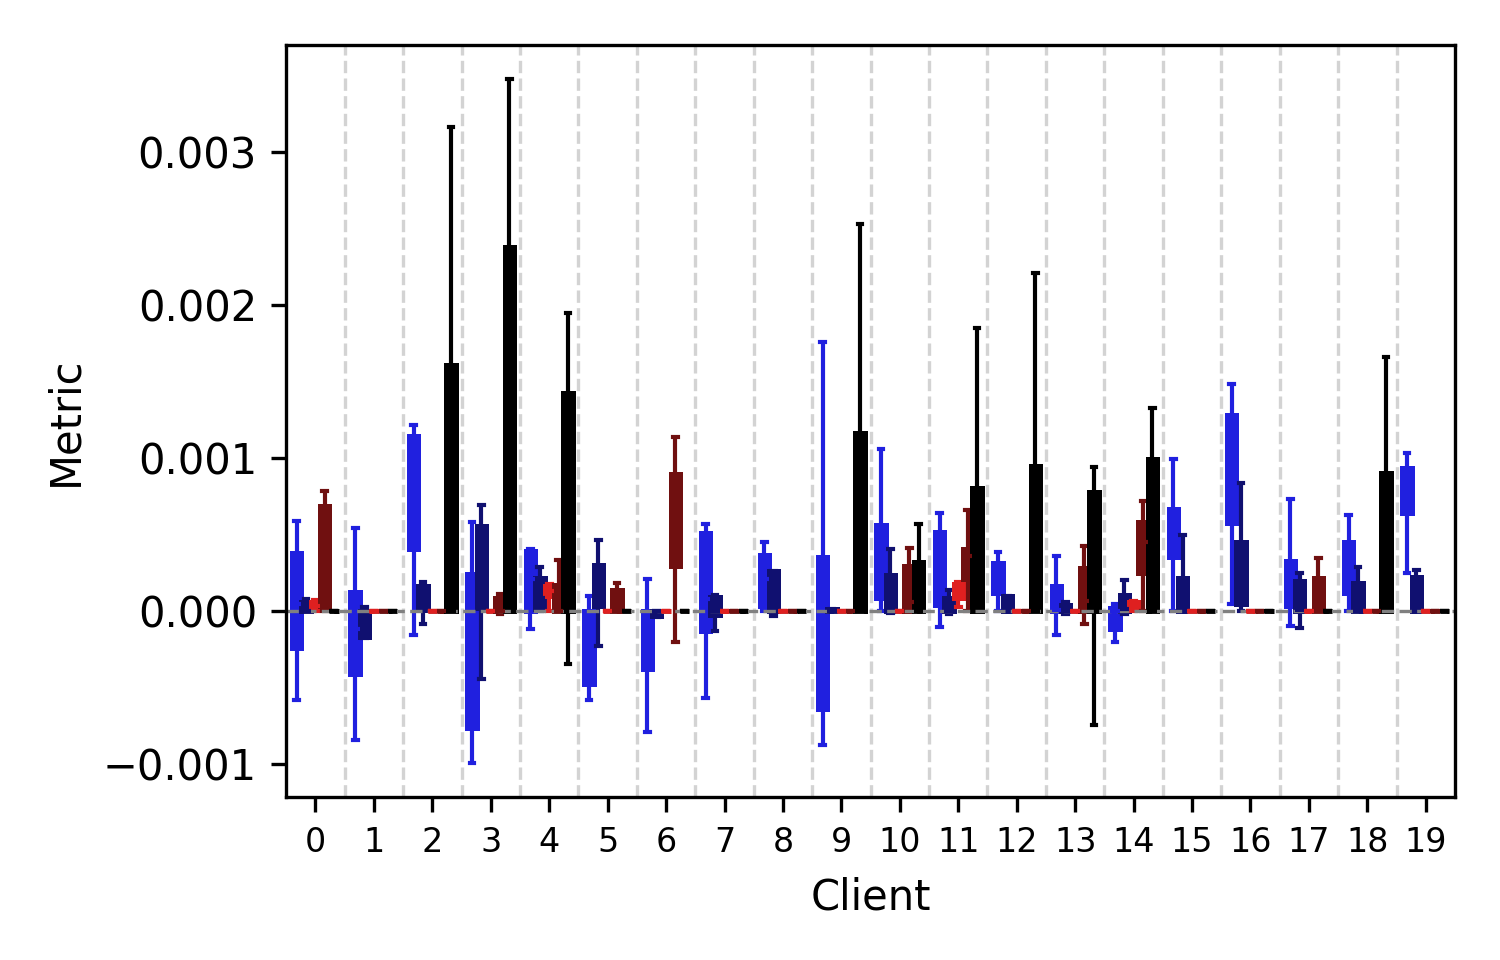
\includegraphics[width=\linewidth]{figs/S_I_20_I_gtg.png}
        \caption{[I]: 20 I / GTG}
    \end{subfigure}
    \hfill
    \begin{subfigure}{0.24\linewidth}
        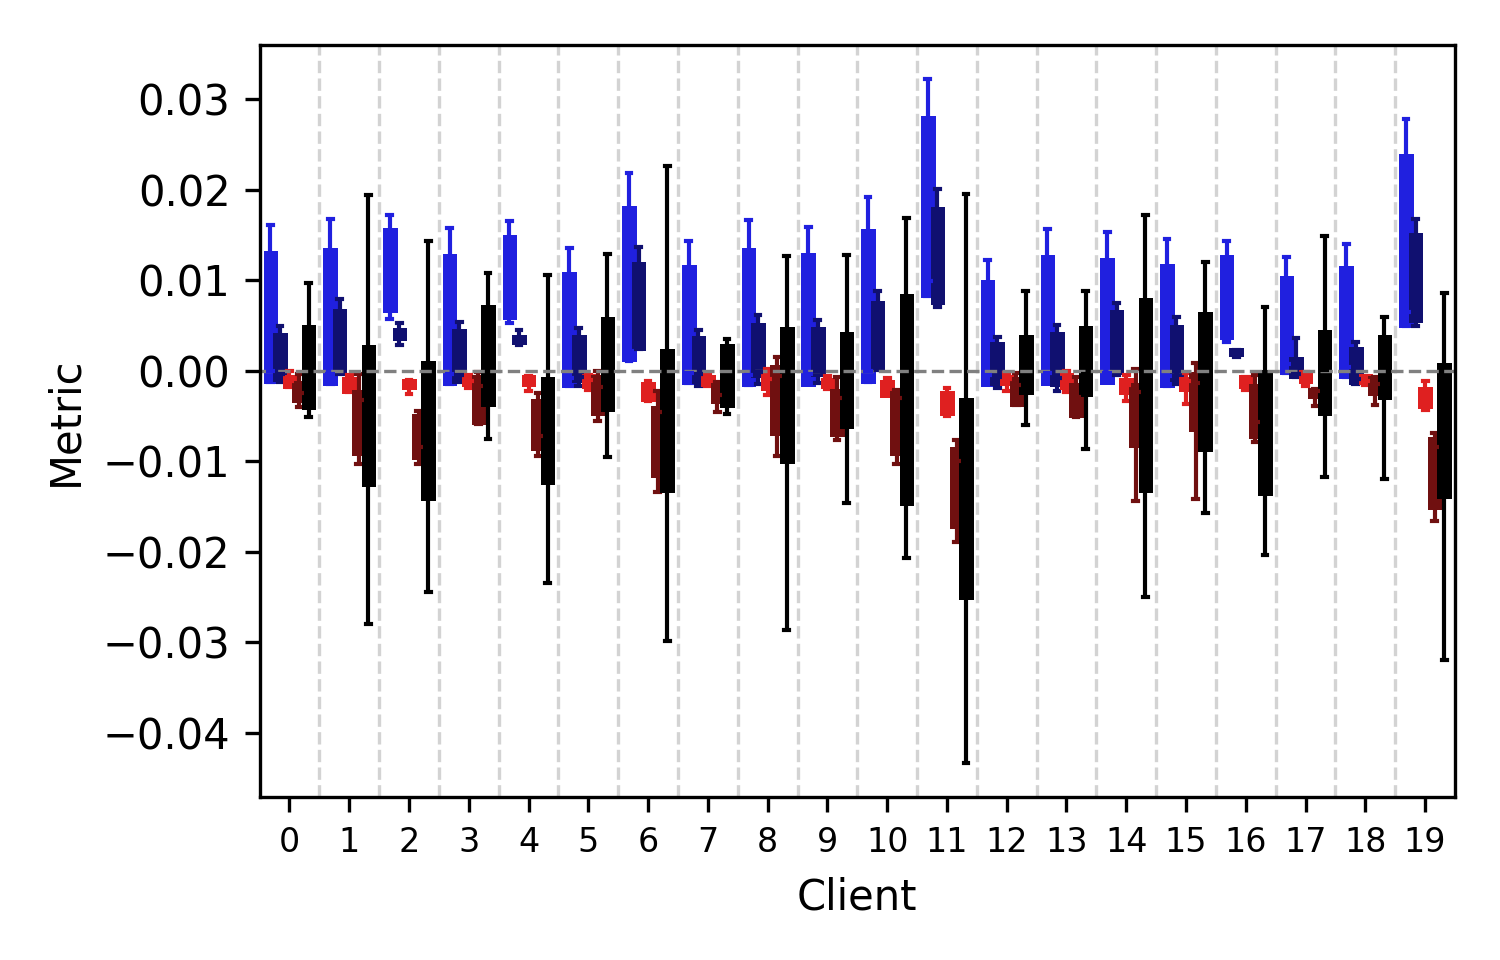
\includegraphics[width=\linewidth]{figs/S_I_20_N_l1o.png}
        \caption{[I]: 20 N / LOO}
    \end{subfigure}
    \hfill
    \begin{subfigure}{0.24\linewidth}
        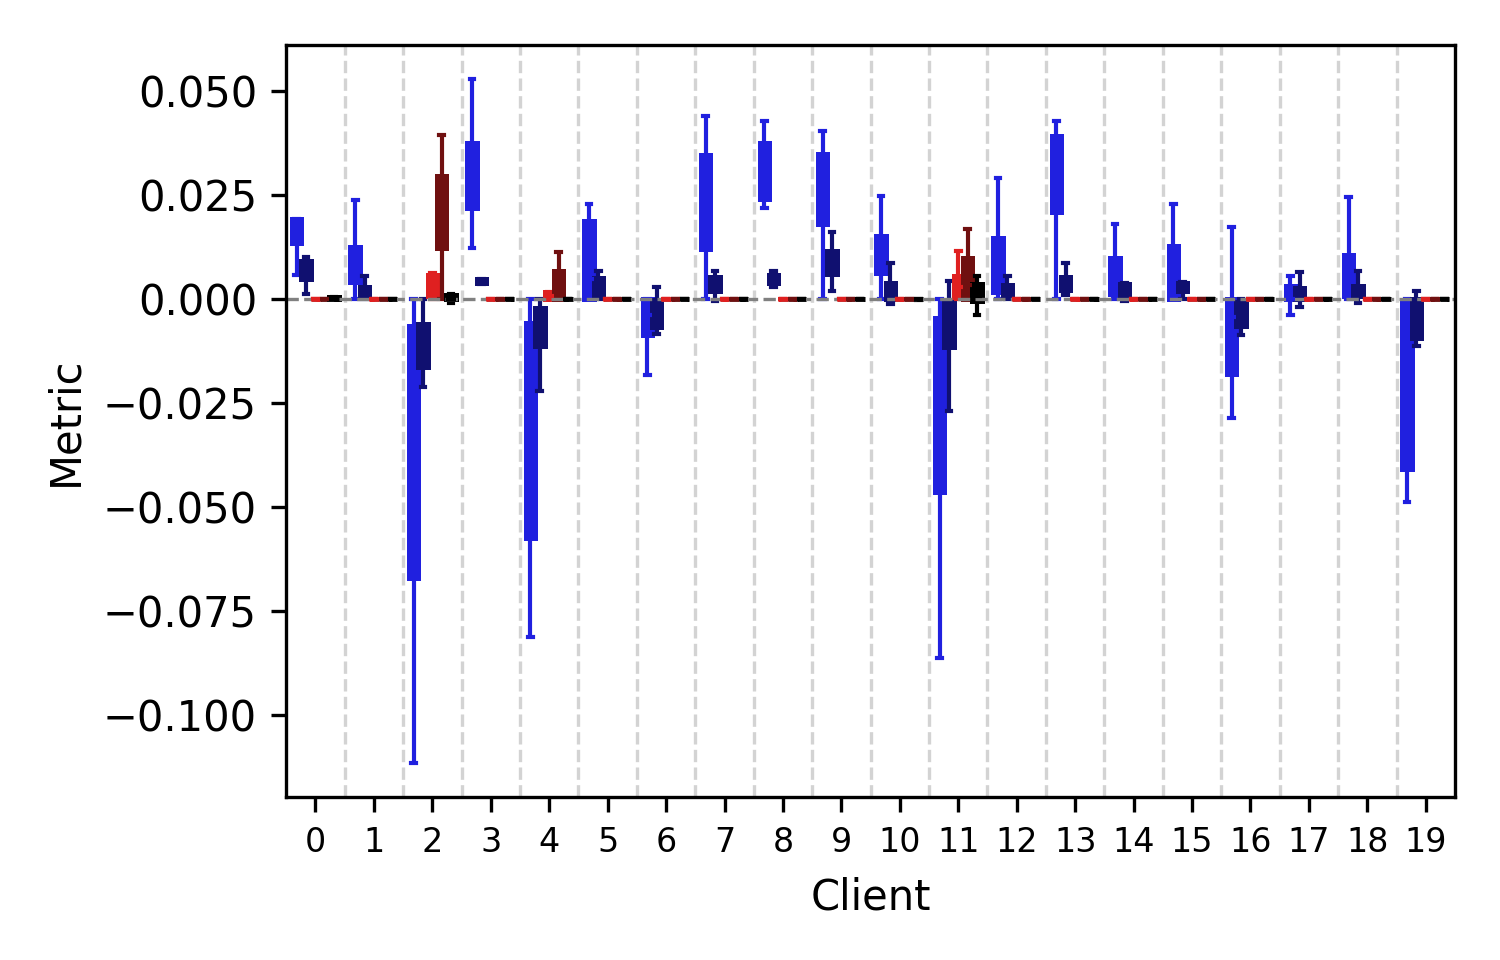
\includegraphics[width=\linewidth]{figs/S_I_20_N_gtg.png}
        \caption{[I]: 20 N / GTG}
    \end{subfigure}
    
    \caption{Empirical score distributions (round $t=10$) for the 4-client scenario where [A], [C], and [I] are ADULT, CelebA. and IMDB.}
    % ADULT - 4 Clients
    \begin{subfigure}{0.24\linewidth}
        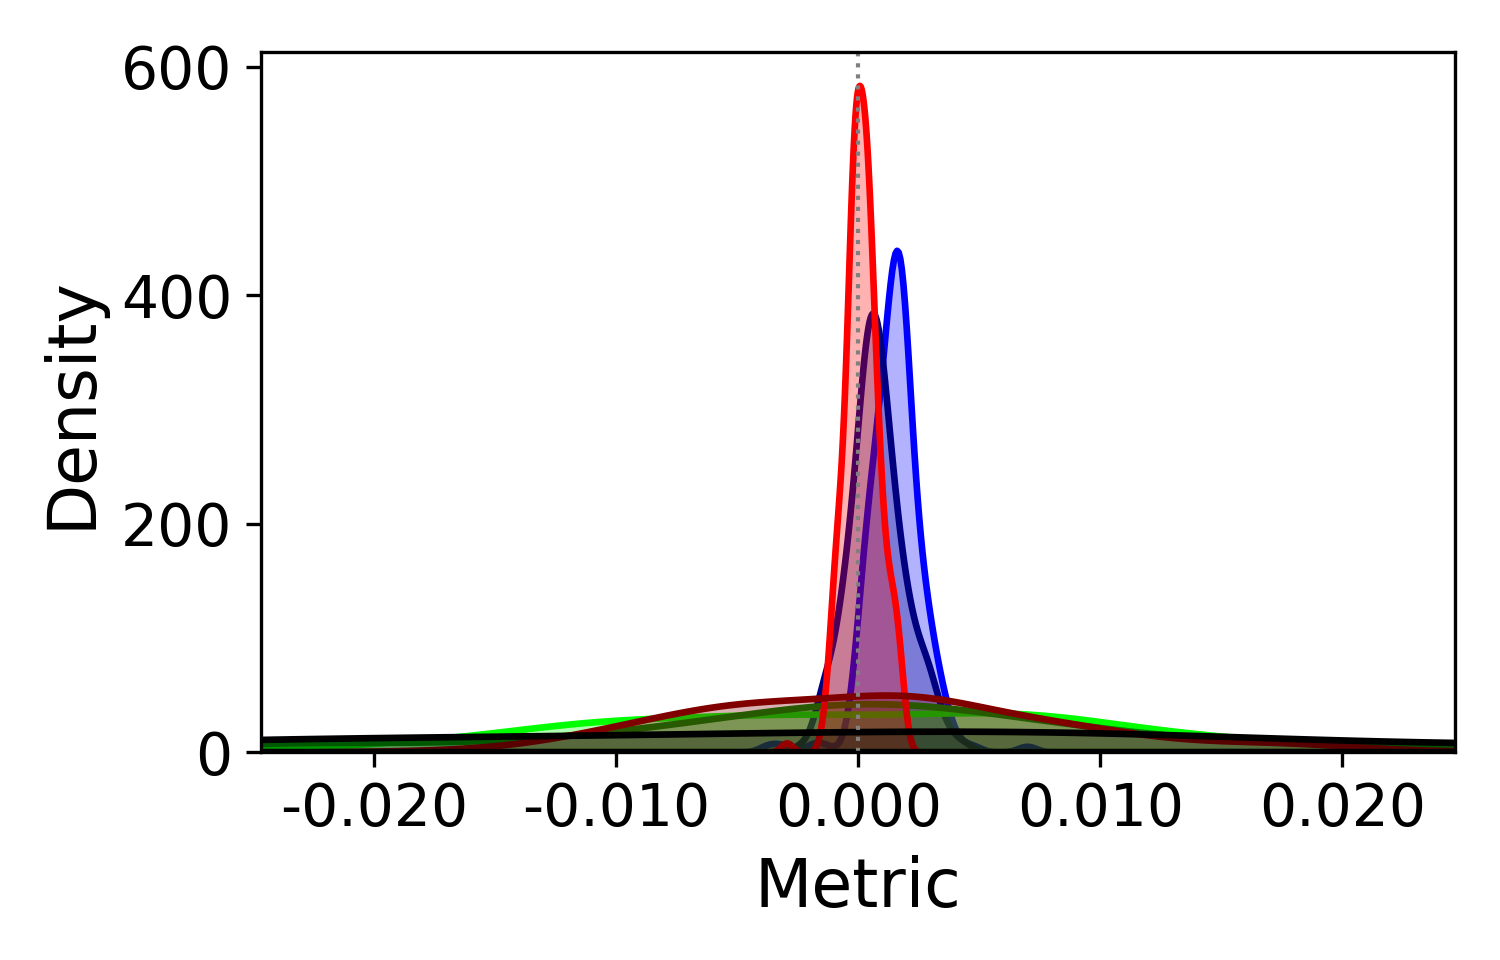
\includegraphics[width=\linewidth]{figs/SD_4_A_I_l1o.png}
        \caption{[A]: IID / LOO}
    \end{subfigure}
    \hfill
    \begin{subfigure}{0.24\linewidth}
        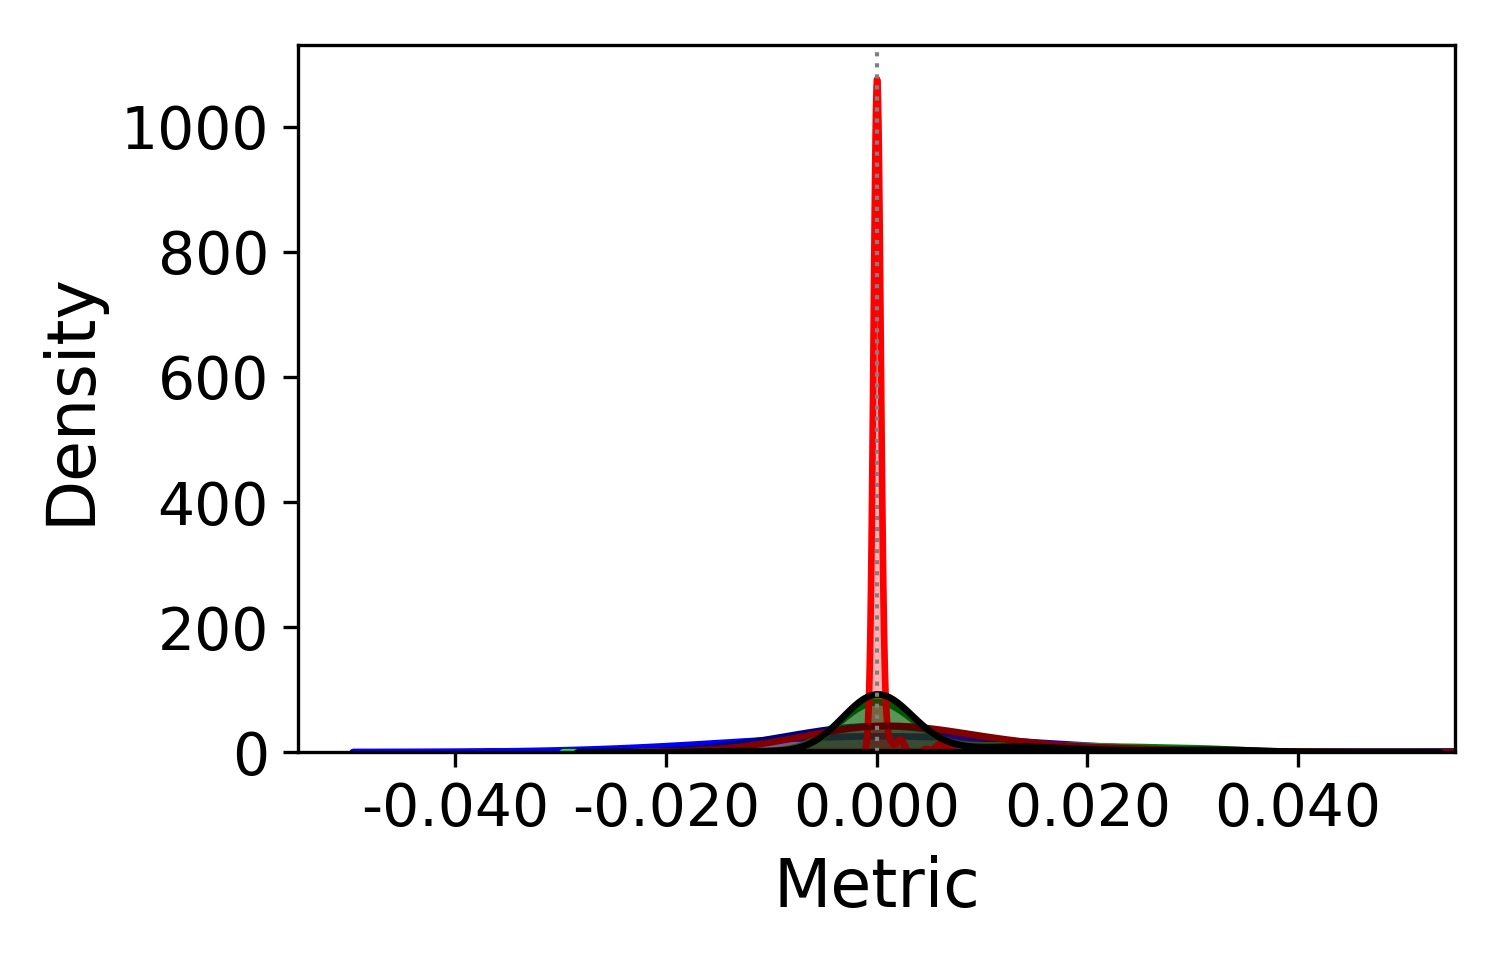
\includegraphics[width=\linewidth]{figs/SD_4_A_I_gtg.png}
        \caption{[A]: IID / GTG}
    \end{subfigure}
    \hfill
    \begin{subfigure}{0.24\linewidth}
        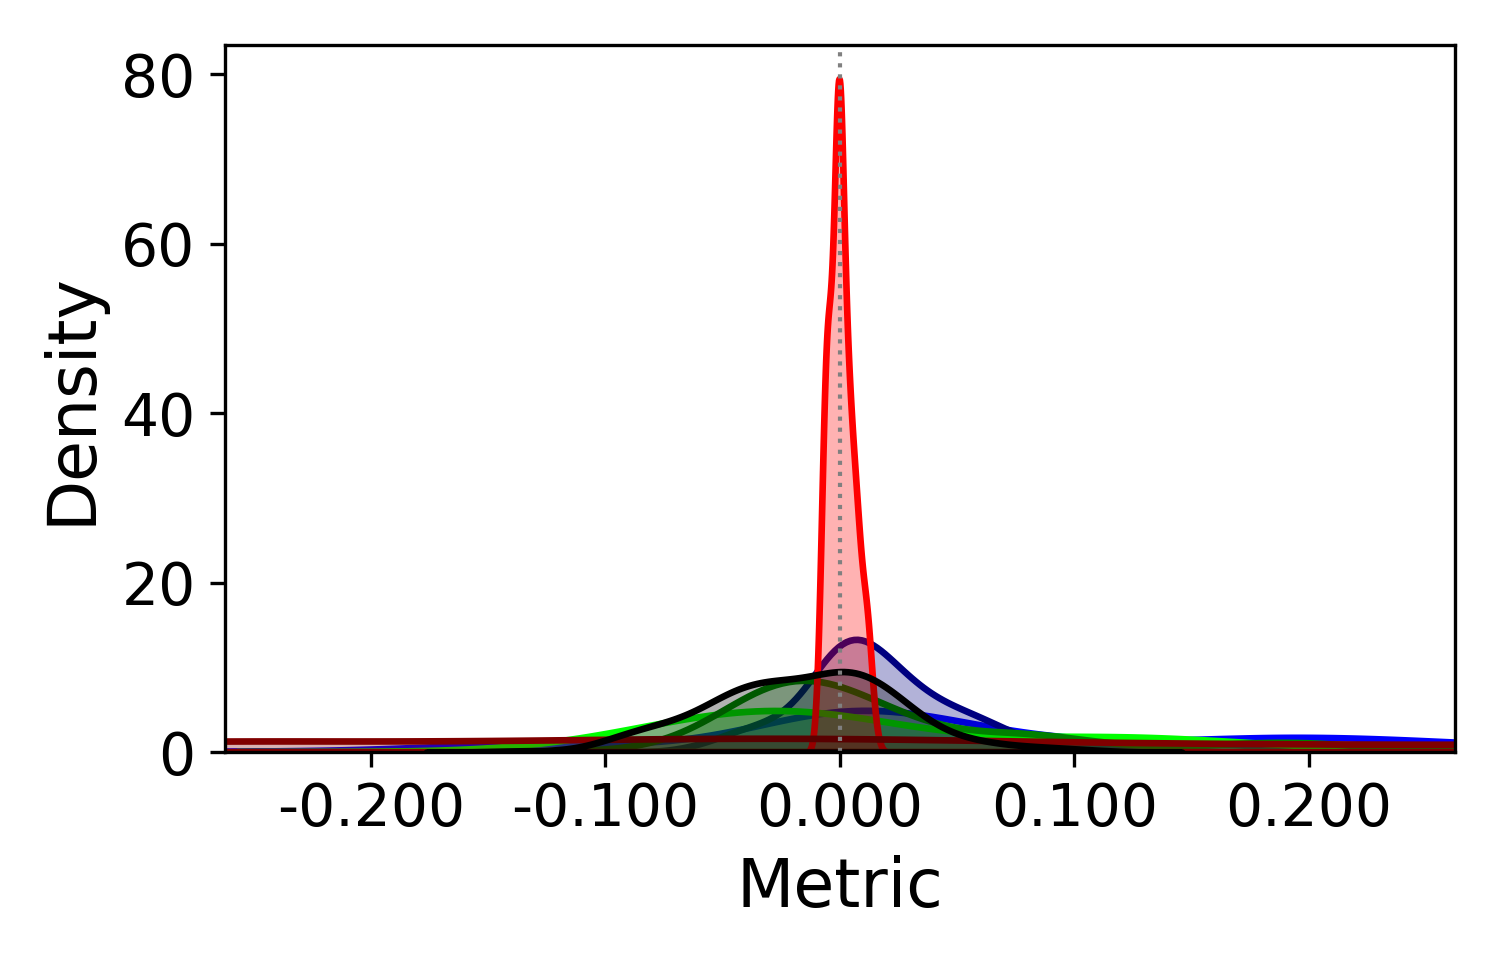
\includegraphics[width=\linewidth]{figs/SD_4_A_N_l1o.png}
        \caption{[A]: NIID / LOO}
    \end{subfigure}
    \hfill
    \begin{subfigure}{0.24\linewidth}
        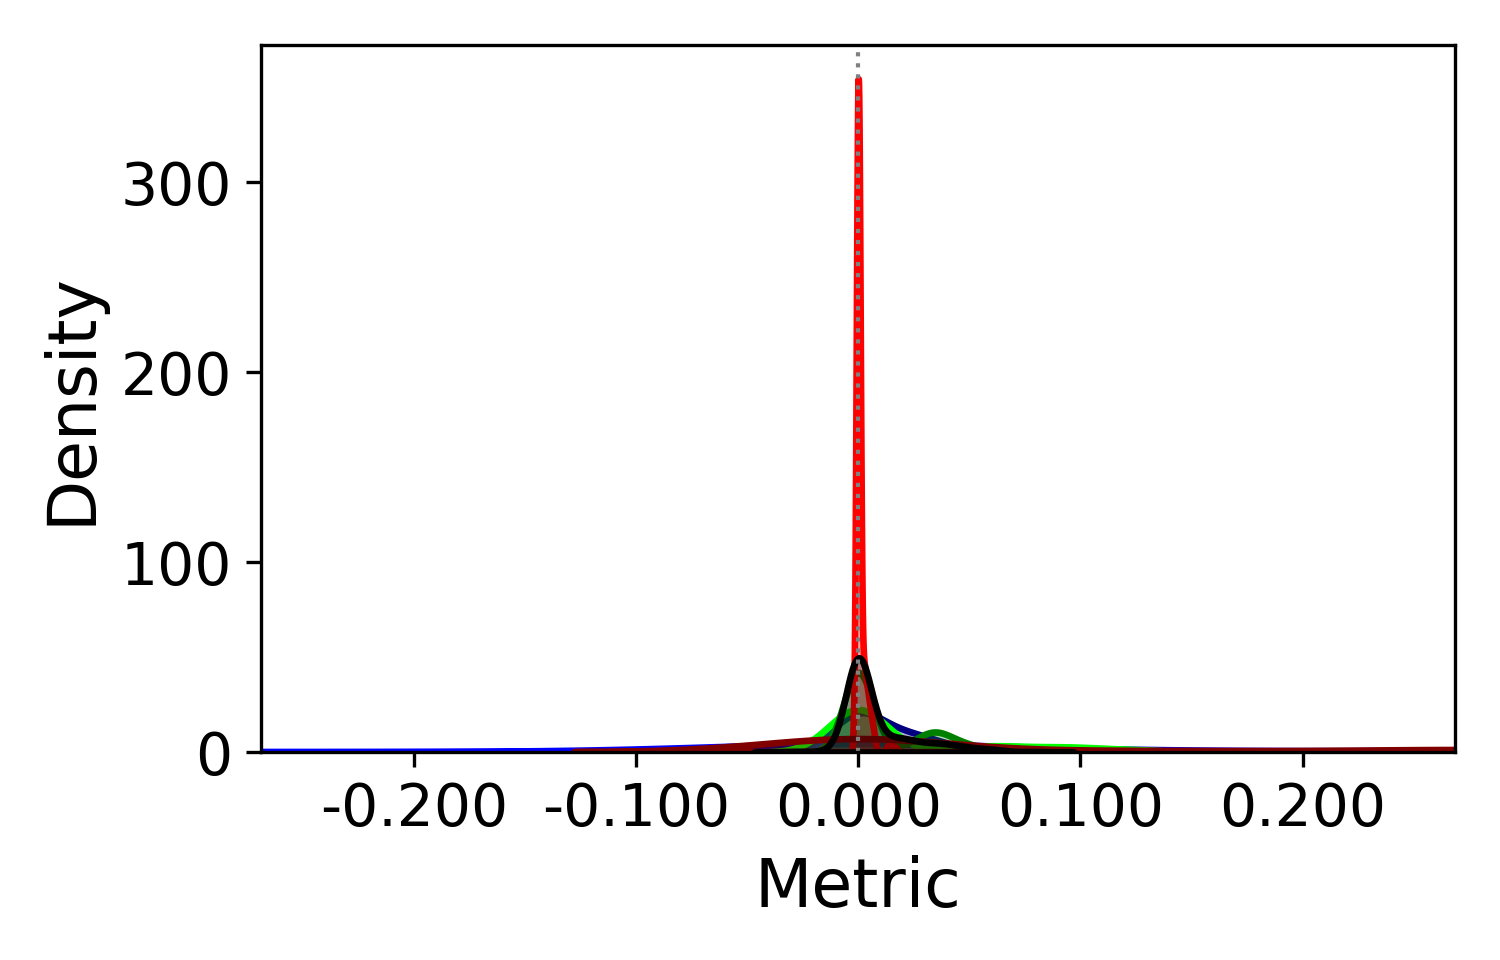
\includegraphics[width=\linewidth]{figs/SD_4_A_N_gtg.png}
        \caption{[A]: NIID / GTG}
    \end{subfigure}

    % CelebA - 4 Clients
    \begin{subfigure}{0.24\linewidth}
        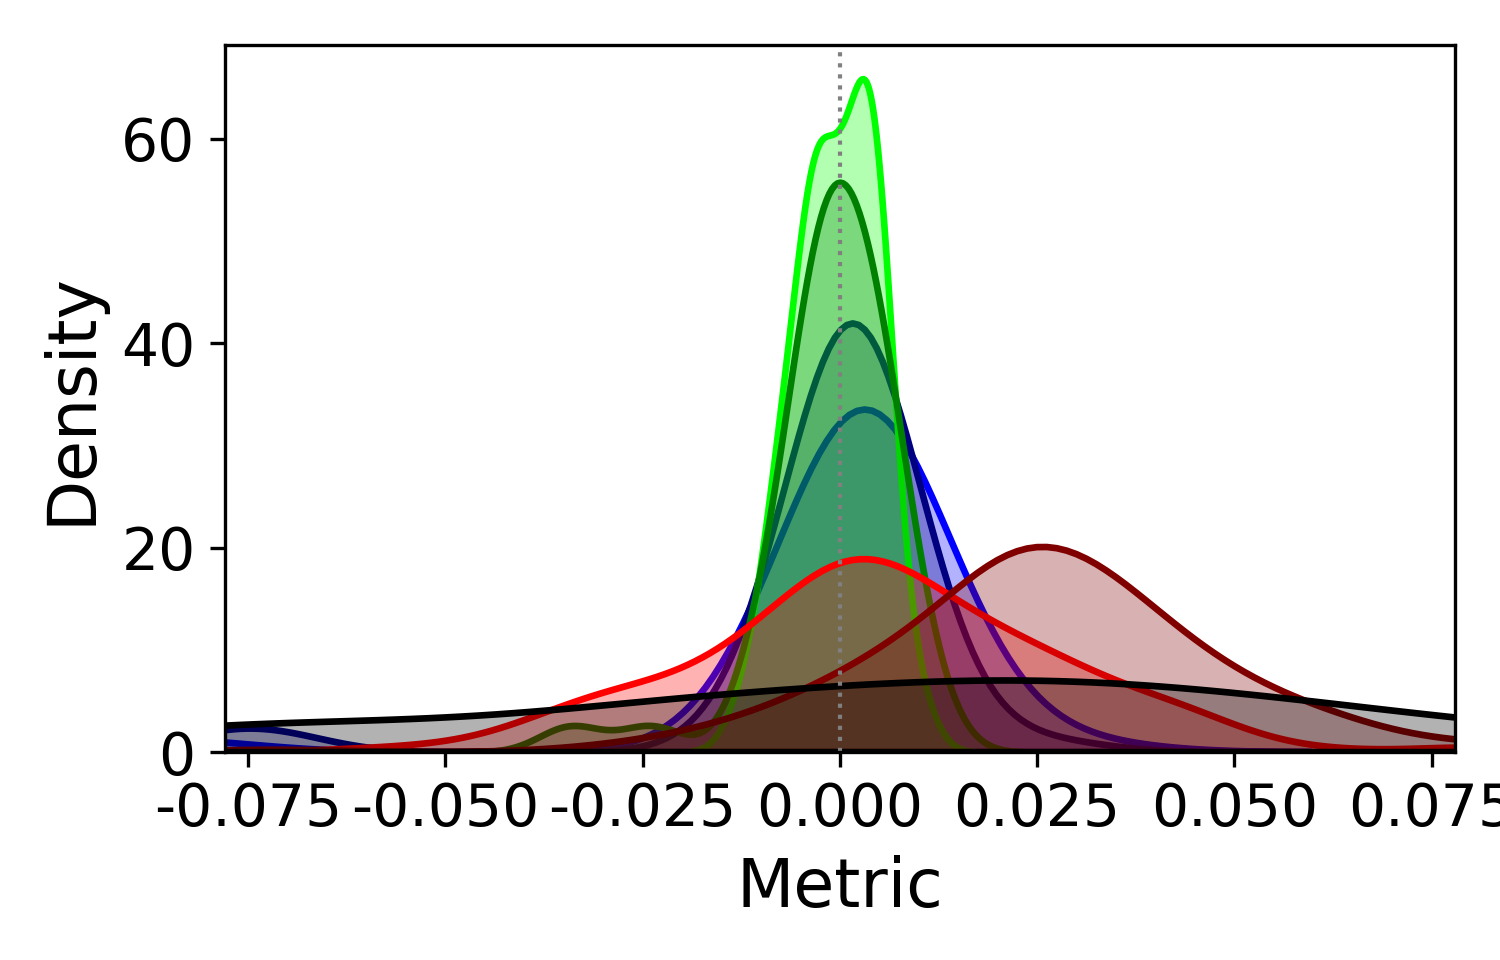
\includegraphics[width=\linewidth]{figs/SD_4_C_I_l1o.png}
        \caption{[C]: IID / LOO}
    \end{subfigure}
    \hfill
    \begin{subfigure}{0.24\linewidth}
        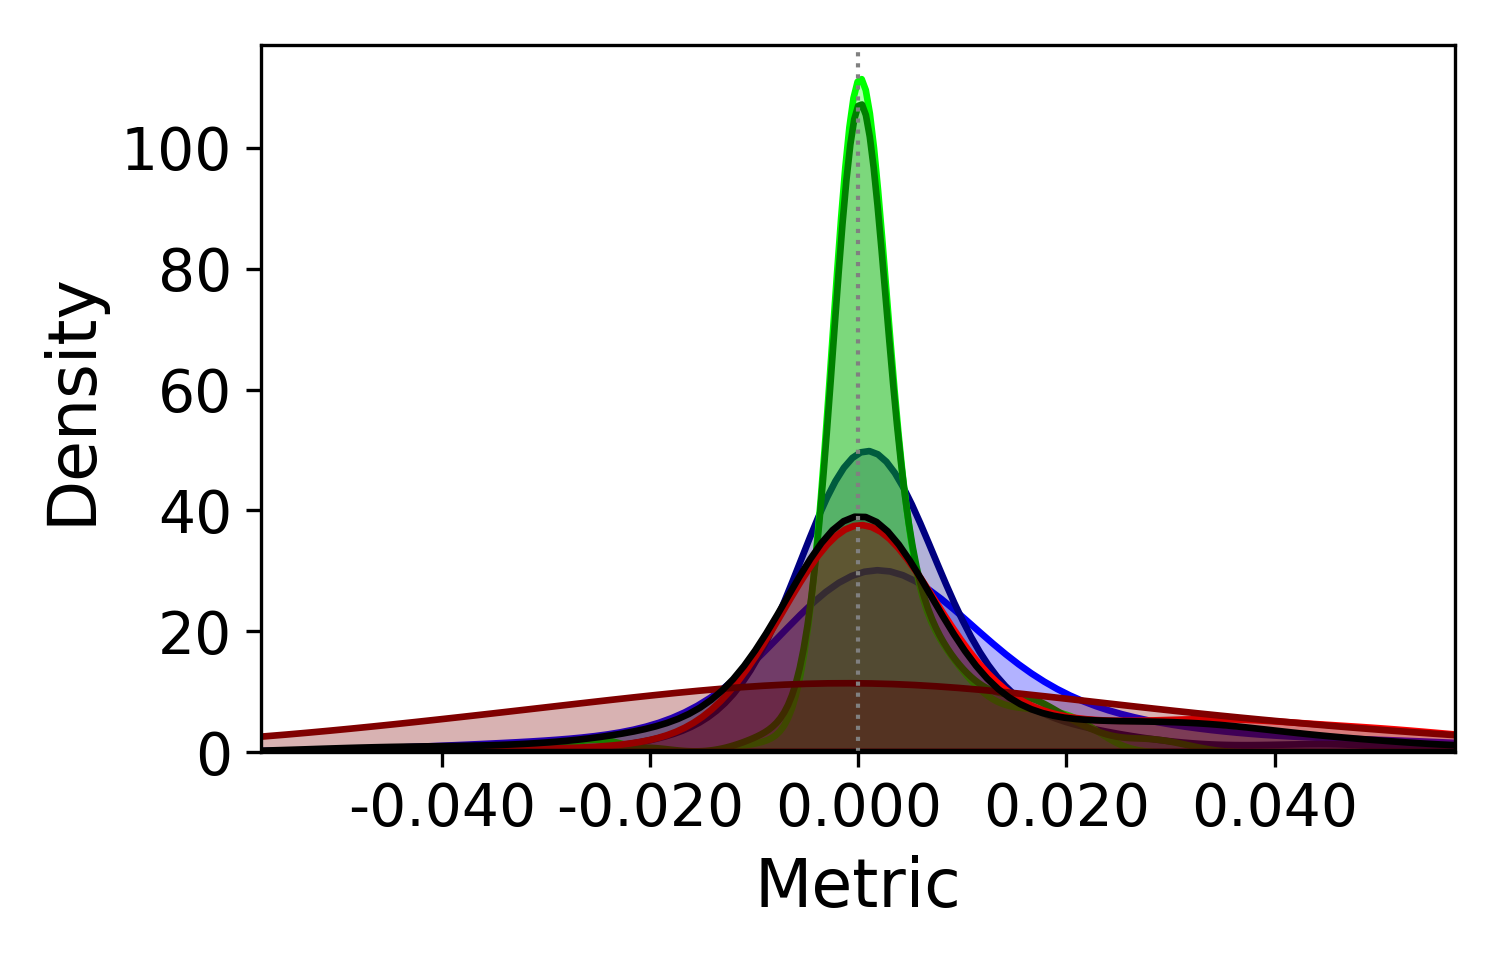
\includegraphics[width=\linewidth]{figs/SD_4_C_I_gtg.png}
        \caption{[C]: IID / GTG}
    \end{subfigure}
    \hfill
    \begin{subfigure}{0.24\linewidth}
        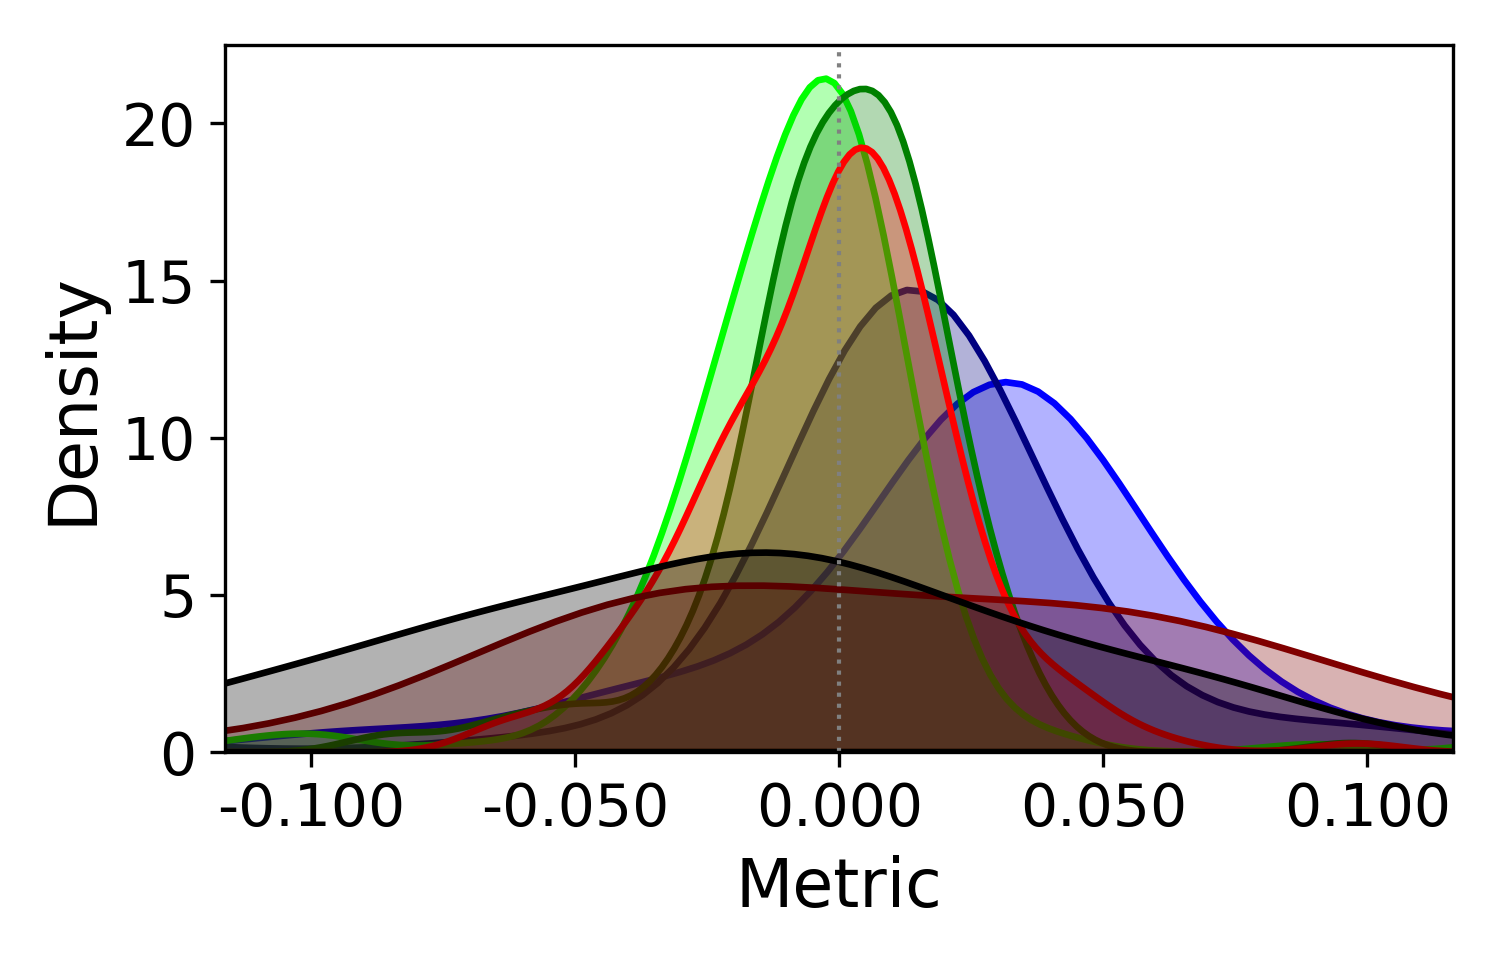
\includegraphics[width=\linewidth]{figs/SD_4_C_N_l1o.png}
        \caption{[C]: NIID / LOO}
    \end{subfigure}
    \hfill
    \begin{subfigure}{0.24\linewidth}
        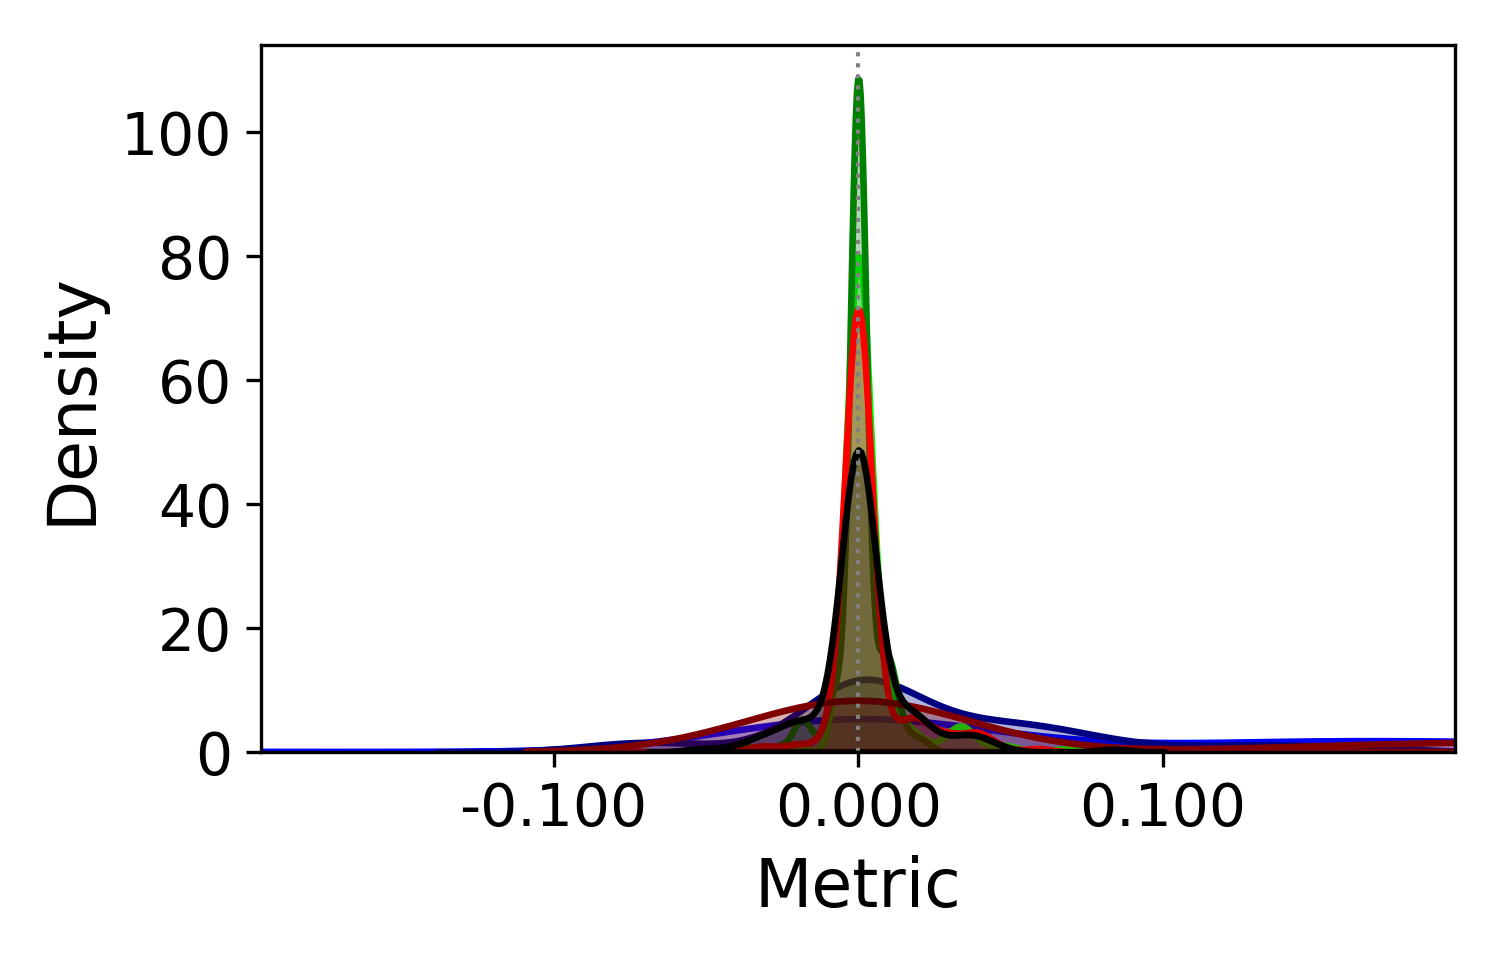
\includegraphics[width=\linewidth]{figs/SD_4_C_N_gtg.png}
        \caption{[C]: NIID / GTG}
    \end{subfigure}

    % IMDB - 4 Clients
    \begin{subfigure}{0.24\linewidth}
        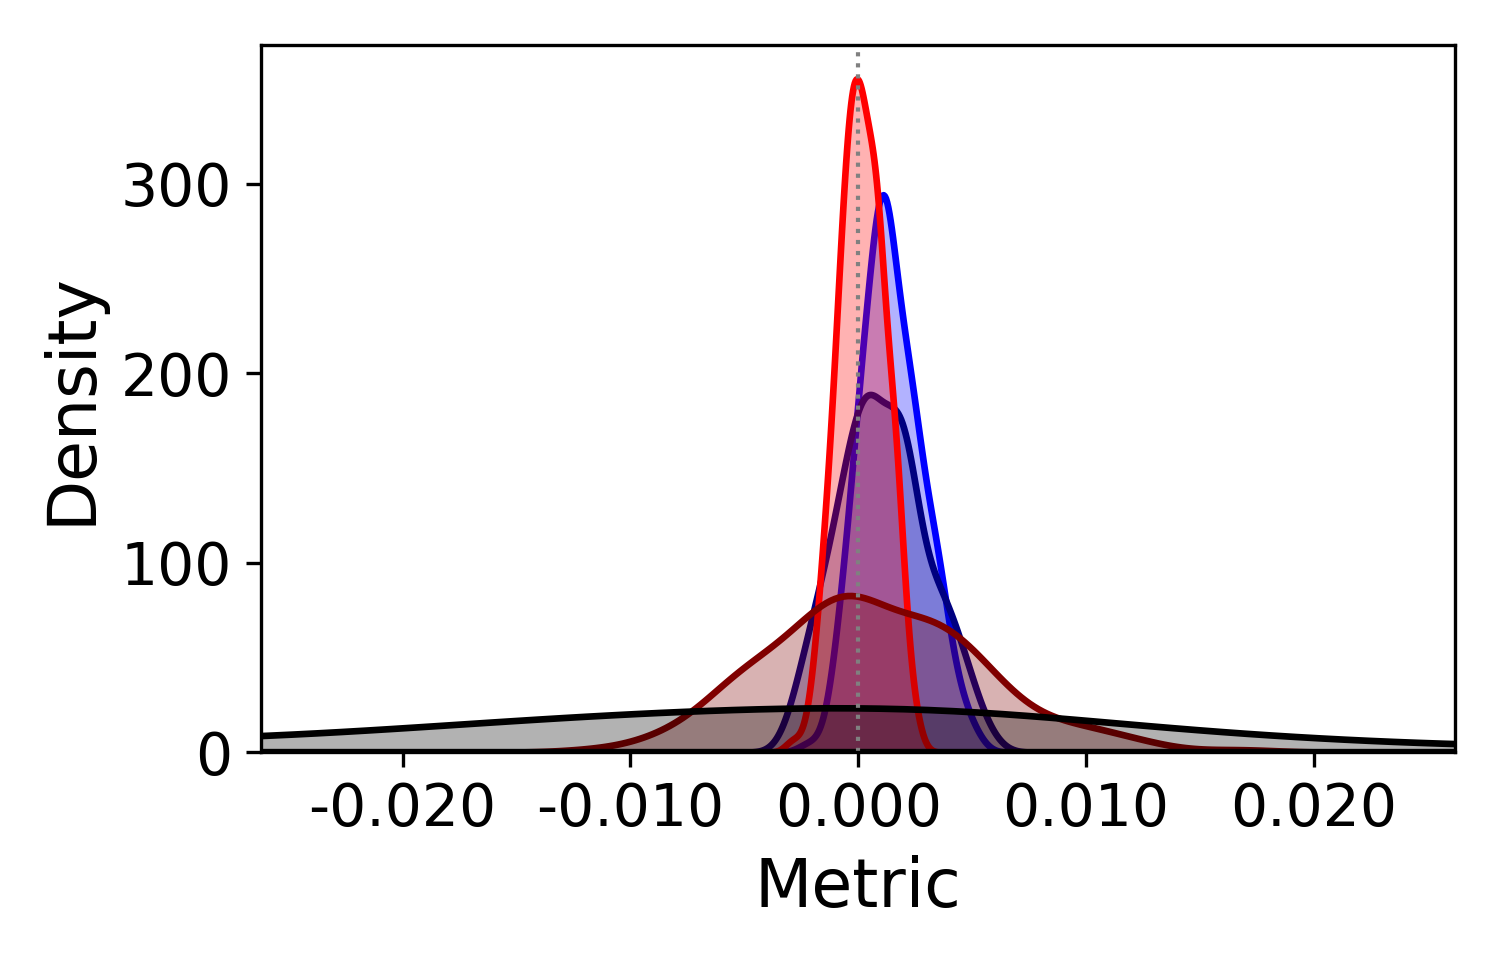
\includegraphics[width=\linewidth]{figs/SD_4_I_I_l1o.png}
        \caption{[I]: IID / LOO}
    \end{subfigure}
    \hfill
    \begin{subfigure}{0.24\linewidth}
        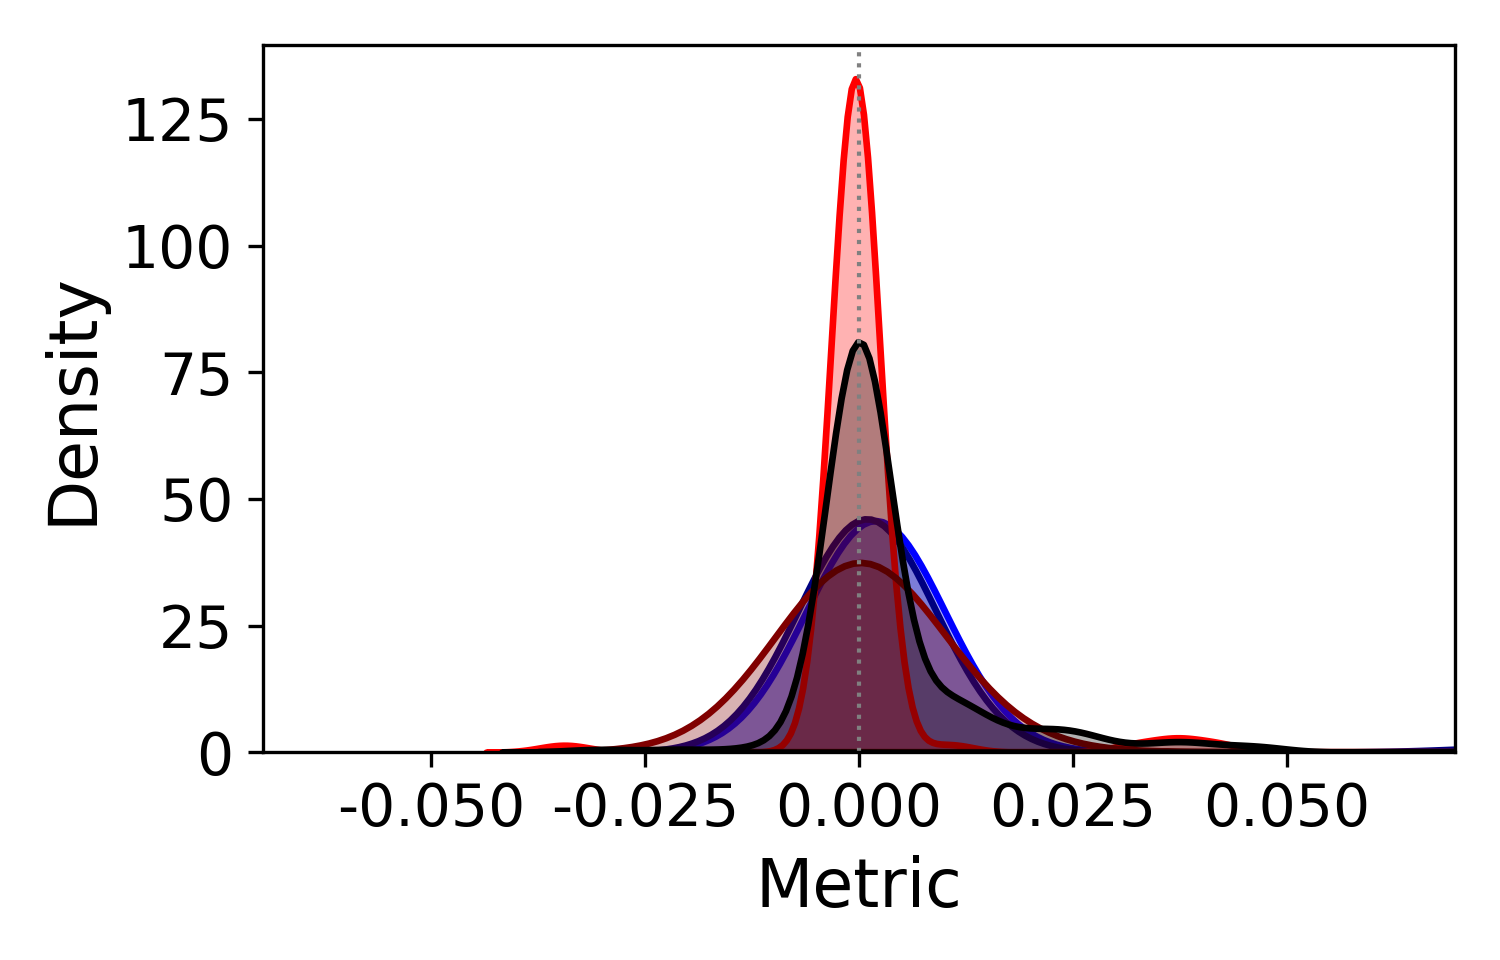
\includegraphics[width=\linewidth]{figs/SD_4_I_I_gtg.png}
        \caption{[I]: IID / GTG}
    \end{subfigure}
    \hfill
    \begin{subfigure}{0.24\linewidth}
        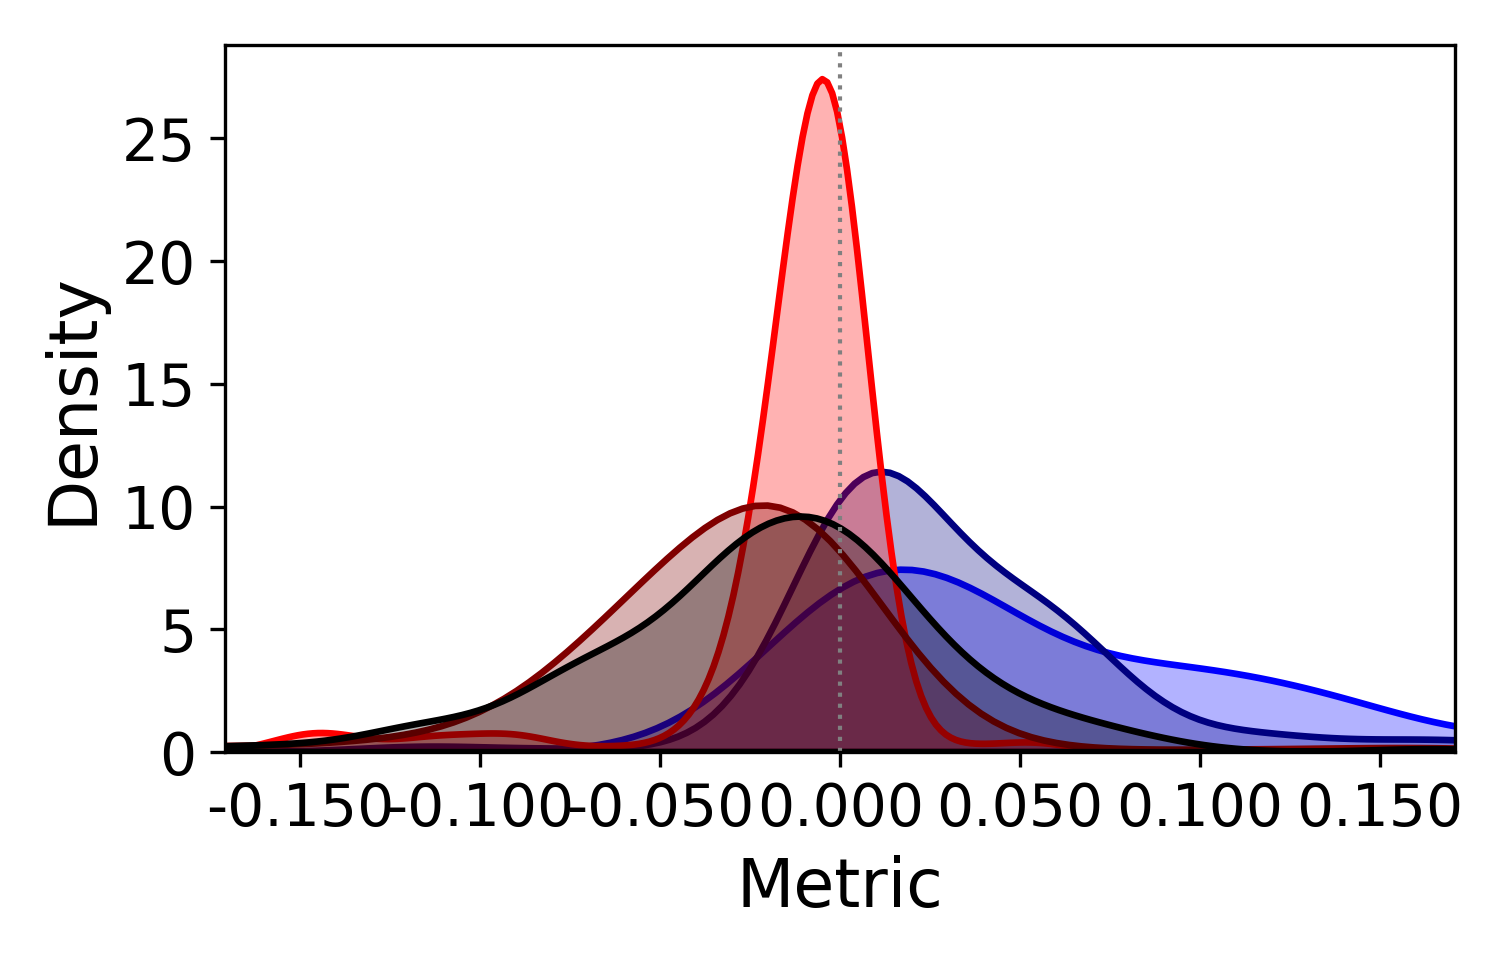
\includegraphics[width=\linewidth]{figs/SD_4_I_N_l1o.png}
        \caption{[I]: NIID / LOO}
    \end{subfigure}
    \hfill
    \begin{subfigure}{0.24\linewidth}
        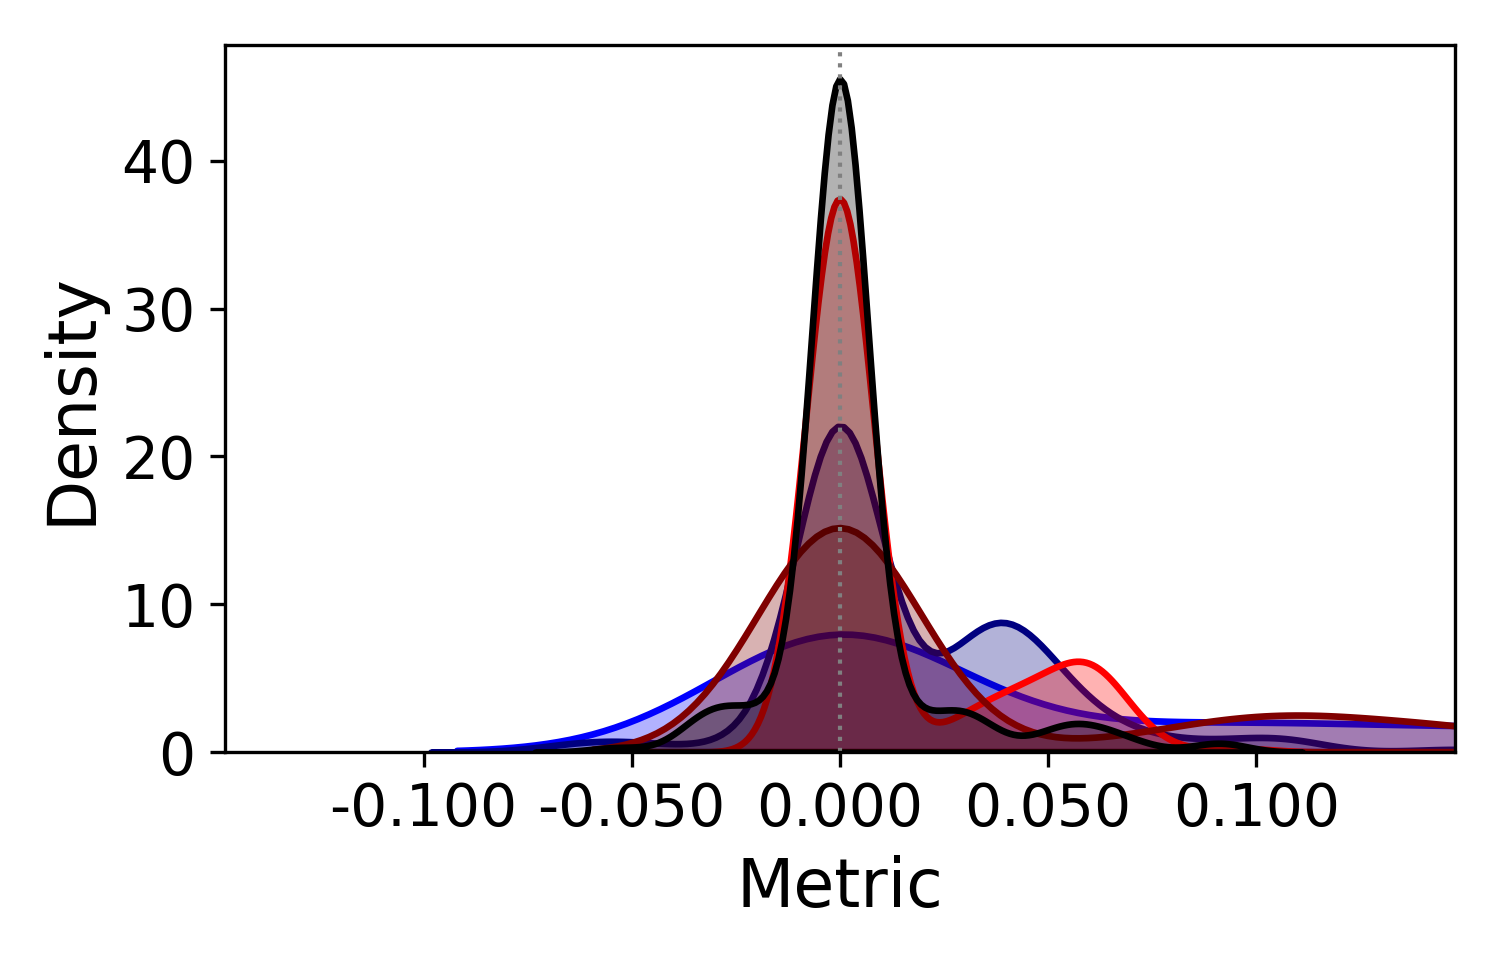
\includegraphics[width=\linewidth]{figs/SD_4_I_N_gtg.png}
        \caption{[I]: NIID / GTG}
    \end{subfigure}
\end{figure}

\end{document}